\documentclass[twoside]{book}

% Packages required by doxygen
\usepackage{fixltx2e}
\usepackage{calc}
\usepackage{doxygen}
\usepackage[export]{adjustbox} % also loads graphicx
\usepackage{graphicx}
\usepackage[utf8]{inputenc}
\usepackage{makeidx}
\usepackage{multicol}
\usepackage{multirow}
\PassOptionsToPackage{warn}{textcomp}
\usepackage{textcomp}
\usepackage[nointegrals]{wasysym}
\usepackage[table]{xcolor}

% Font selection
\usepackage[T1]{fontenc}
\usepackage[scaled=.90]{helvet}
\usepackage{courier}
\usepackage{amssymb}
\usepackage{sectsty}
\renewcommand{\familydefault}{\sfdefault}
\allsectionsfont{%
  \fontseries{bc}\selectfont%
  \color{darkgray}%
}
\renewcommand{\DoxyLabelFont}{%
  \fontseries{bc}\selectfont%
  \color{darkgray}%
}
\newcommand{\+}{\discretionary{\mbox{\scriptsize$\hookleftarrow$}}{}{}}

% Page & text layout
\usepackage{geometry}
\geometry{%
  a4paper,%
  top=2.5cm,%
  bottom=2.5cm,%
  left=2.5cm,%
  right=2.5cm%
}
\tolerance=750
\hfuzz=15pt
\hbadness=750
\setlength{\emergencystretch}{15pt}
\setlength{\parindent}{0cm}
\setlength{\parskip}{3ex plus 2ex minus 2ex}
\makeatletter
\renewcommand{\paragraph}{%
  \@startsection{paragraph}{4}{0ex}{-1.0ex}{1.0ex}{%
    \normalfont\normalsize\bfseries\SS@parafont%
  }%
}
\renewcommand{\subparagraph}{%
  \@startsection{subparagraph}{5}{0ex}{-1.0ex}{1.0ex}{%
    \normalfont\normalsize\bfseries\SS@subparafont%
  }%
}
\makeatother

% Headers & footers
\usepackage{fancyhdr}
\pagestyle{fancyplain}
\fancyhead[LE]{\fancyplain{}{\bfseries\thepage}}
\fancyhead[CE]{\fancyplain{}{}}
\fancyhead[RE]{\fancyplain{}{\bfseries\leftmark}}
\fancyhead[LO]{\fancyplain{}{\bfseries\rightmark}}
\fancyhead[CO]{\fancyplain{}{}}
\fancyhead[RO]{\fancyplain{}{\bfseries\thepage}}
\fancyfoot[LE]{\fancyplain{}{}}
\fancyfoot[CE]{\fancyplain{}{}}
\fancyfoot[RE]{\fancyplain{}{\bfseries\scriptsize Generated by Doxygen }}
\fancyfoot[LO]{\fancyplain{}{\bfseries\scriptsize Generated by Doxygen }}
\fancyfoot[CO]{\fancyplain{}{}}
\fancyfoot[RO]{\fancyplain{}{}}
\renewcommand{\footrulewidth}{0.4pt}
\renewcommand{\chaptermark}[1]{%
  \markboth{#1}{}%
}
\renewcommand{\sectionmark}[1]{%
  \markright{\thesection\ #1}%
}

% Indices & bibliography
\usepackage{natbib}
\usepackage[titles]{tocloft}
\setcounter{tocdepth}{3}
\setcounter{secnumdepth}{5}
\makeindex

% Hyperlinks (required, but should be loaded last)
\usepackage{ifpdf}
\ifpdf
  \usepackage[pdftex,pagebackref=true]{hyperref}
\else
  \usepackage[ps2pdf,pagebackref=true]{hyperref}
\fi
\hypersetup{%
  colorlinks=true,%
  linkcolor=blue,%
  citecolor=blue,%
  unicode%
}

% Custom commands
\newcommand{\clearemptydoublepage}{%
  \newpage{\pagestyle{empty}\cleardoublepage}%
}

\usepackage{caption}
\captionsetup{labelsep=space,justification=centering,font={bf},singlelinecheck=off,skip=4pt,position=top}

%===== C O N T E N T S =====

\begin{document}

% Titlepage & ToC
\hypersetup{pageanchor=false,
             bookmarksnumbered=true,
             pdfencoding=unicode
            }
\pagenumbering{alph}
\begin{titlepage}
\vspace*{7cm}
\begin{center}%
{\Large Radio Controller Code }\\
\vspace*{1cm}
{\large Generated by Doxygen 1.8.13}\\
\end{center}
\end{titlepage}
\clearemptydoublepage
\pagenumbering{roman}
\tableofcontents
\clearemptydoublepage
\pagenumbering{arabic}
\hypersetup{pageanchor=true}

%--- Begin generated contents ---
\chapter{Namespace Index}
\section{Namespace List}
Here is a list of all documented namespaces with brief descriptions\+:\begin{DoxyCompactList}
\item\contentsline{section}{\hyperlink{namespacemath_functions}{math\+Functions} \\*Collection of useful templated math functions }{\pageref{namespacemath_functions}}{}
\end{DoxyCompactList}

\chapter{Hierarchical Index}
\section{Class Hierarchy}
This inheritance list is sorted roughly, but not completely, alphabetically\+:\begin{DoxyCompactList}
\item \contentsline{section}{Battery}{\pageref{class_battery}}{}
\item \contentsline{section}{battery}{\pageref{classbattery}}{}
\item \contentsline{section}{Button}{\pageref{class_button}}{}
\begin{DoxyCompactList}
\item \contentsline{section}{Switch}{\pageref{class_switch}}{}
\end{DoxyCompactList}
\item \contentsline{section}{Buzzer}{\pageref{class_buzzer}}{}
\item \contentsline{section}{Encoder}{\pageref{class_encoder}}{}
\item \contentsline{section}{Joystick}{\pageref{class_joystick}}{}
\item \contentsline{section}{Led}{\pageref{class_led}}{}
\item \contentsline{section}{Plane\+Battery\+Bisplay}{\pageref{class_plane_battery_bisplay}}{}
\item \contentsline{section}{R\+G\+B\+Led}{\pageref{class_r_g_b_led}}{}
\item \contentsline{section}{Sevseg\+Screen}{\pageref{class_sevseg_screen}}{}
\end{DoxyCompactList}

\chapter{Class Index}
\section{Class List}
Here are the classes, structs, unions and interfaces with brief descriptions\+:\begin{DoxyCompactList}
\item\contentsline{section}{\hyperlink{class_battery}{Battery} }{\pageref{class_battery}}{}
\item\contentsline{section}{\hyperlink{classbattery}{battery} \\*Represents the Lipo battery pack and implements methods to get its charge level }{\pageref{classbattery}}{}
\item\contentsline{section}{\hyperlink{class_button}{Button} \\*\hyperlink{class_button}{Button} class is responsible for reading a pushbutton state with debounce feature }{\pageref{class_button}}{}
\item\contentsline{section}{\hyperlink{class_buzzer}{Buzzer} \\*\hyperlink{class_buzzer}{Buzzer} class is responsible for sound outputs }{\pageref{class_buzzer}}{}
\item\contentsline{section}{\hyperlink{class_control}{Control} \\*\hyperlink{class_control}{Control} class is responsible for translating \hyperlink{class_joystick}{Joystick}, encoder and button inputs into power, pitch, yaw and roll values }{\pageref{class_control}}{}
\item\contentsline{section}{\hyperlink{class_encoder}{Encoder} \\*\hyperlink{class_encoder}{Encoder} class is responsible for reading rotary encoder input }{\pageref{class_encoder}}{}
\item\contentsline{section}{\hyperlink{class_joystick}{Joystick} }{\pageref{class_joystick}}{}
\item\contentsline{section}{\hyperlink{class_l_c_d_screen}{L\+C\+D\+Screen} \\*\hyperlink{class_l_c_d_screen}{L\+C\+D\+Screen} class is responsible for displaying informations on an S\+S\+D1306 I2C screen }{\pageref{class_l_c_d_screen}}{}
\item\contentsline{section}{\hyperlink{class_led}{Led} }{\pageref{class_led}}{}
\item\contentsline{section}{\hyperlink{class_plane_battery_bisplay}{Plane\+Battery\+Bisplay} \\*Responsible for displaying battery informations }{\pageref{class_plane_battery_bisplay}}{}
\item\contentsline{section}{\hyperlink{struct_pto_t_data_frame}{Pto\+T\+Data\+Frame} \\*Struct composed with all data contained in a frame sent from the Plane to the Transmitter }{\pageref{struct_pto_t_data_frame}}{}
\item\contentsline{section}{\hyperlink{class_radio}{Radio} \\*\hyperlink{class_radio}{Radio} class responsible for communicating with the \hyperlink{class_radio}{Radio} Transmitter on the ground }{\pageref{class_radio}}{}
\item\contentsline{section}{\hyperlink{class_remote_battery}{Remote\+Battery} }{\pageref{class_remote_battery}}{}
\item\contentsline{section}{\hyperlink{class_r_g_b_led}{R\+G\+B\+Led} \\*\hyperlink{class_r_g_b_led}{R\+G\+B\+Led} class is responsible for displaying colors on an R\+GB \hyperlink{class_led}{Led} }{\pageref{class_r_g_b_led}}{}
\item\contentsline{section}{\hyperlink{class_settings}{Settings} \\*\hyperlink{class_settings}{Settings} class is responsible for }{\pageref{class_settings}}{}
\item\contentsline{section}{\hyperlink{class_sevseg_screen}{Sevseg\+Screen} \\*\hyperlink{class_sevseg_screen}{Sevseg\+Screen} class is responsible for displaying content on a 7-\/segment display }{\pageref{class_sevseg_screen}}{}
\item\contentsline{section}{\hyperlink{class_switch}{Switch} }{\pageref{class_switch}}{}
\item\contentsline{section}{\hyperlink{struct_tto_p_data_frame}{Tto\+P\+Data\+Frame} \\*Struct composed with all data contained in a frame sent from the Transmitter to the Plane }{\pageref{struct_tto_p_data_frame}}{}
\end{DoxyCompactList}

\chapter{File Index}
\section{File List}
Here is a list of all documented files with brief descriptions\+:\begin{DoxyCompactList}
\item\contentsline{section}{src/main/\hyperlink{battery_8cpp}{battery.\+cpp} \\*Definition of battery class }{\pageref{battery_8cpp}}{}
\item\contentsline{section}{src/main/\hyperlink{battery_8h}{battery.\+h} \\*Declaration of battery class }{\pageref{battery_8h}}{}
\item\contentsline{section}{src/main/\hyperlink{button_8cpp}{button.\+cpp} \\*Definition of \hyperlink{class_button}{Button} class }{\pageref{button_8cpp}}{}
\item\contentsline{section}{src/main/\hyperlink{button_8h}{button.\+h} \\*Declaration of \hyperlink{class_button}{Button} class }{\pageref{button_8h}}{}
\item\contentsline{section}{src/main/\hyperlink{buzzer_8cpp}{buzzer.\+cpp} \\*Definition of buzzer class }{\pageref{buzzer_8cpp}}{}
\item\contentsline{section}{src/main/\hyperlink{buzzer_8h}{buzzer.\+h} \\*Declaration of \hyperlink{class_buzzer}{Buzzer} class }{\pageref{buzzer_8h}}{}
\item\contentsline{section}{src/main/\hyperlink{control_8cpp}{control.\+cpp} \\*Definition of control class }{\pageref{control_8cpp}}{}
\item\contentsline{section}{src/main/\hyperlink{control_8h}{control.\+h} \\*Declaration of control class }{\pageref{control_8h}}{}
\item\contentsline{section}{src/main/\hyperlink{encoder_8cpp}{encoder.\+cpp} \\*Definition of \hyperlink{class_encoder}{Encoder} class }{\pageref{encoder_8cpp}}{}
\item\contentsline{section}{src/main/\hyperlink{encoder_8h}{encoder.\+h} \\*Declaration of \hyperlink{class_encoder}{Encoder} class }{\pageref{encoder_8h}}{}
\item\contentsline{section}{src/main/\hyperlink{frame_8h}{frame.\+h} \\*Declaration of frame types and incoming\+Frame class }{\pageref{frame_8h}}{}
\item\contentsline{section}{src/main/{\bfseries header.\+h} }{\pageref{header_8h}}{}
\item\contentsline{section}{src/main/\hyperlink{joystick_8cpp}{joystick.\+cpp} \\*Definition of \hyperlink{class_joystick}{Joystick} class }{\pageref{joystick_8cpp}}{}
\item\contentsline{section}{src/main/\hyperlink{joystick_8h}{joystick.\+h} \\*Declaration of \hyperlink{class_joystick}{Joystick} class }{\pageref{joystick_8h}}{}
\item\contentsline{section}{src/main/\hyperlink{lcd__bitmaps_8h}{lcd\+\_\+bitmaps.\+h} \\*Contain arrays describing btmaps do display on main L\+CD }{\pageref{lcd__bitmaps_8h}}{}
\item\contentsline{section}{src/main/\hyperlink{lcdscreen_8cpp}{lcdscreen.\+cpp} \\*Definition of \hyperlink{class_l_c_d_screen}{L\+C\+D\+Screen} class }{\pageref{lcdscreen_8cpp}}{}
\item\contentsline{section}{src/main/\hyperlink{lcdscreen_8h}{lcdscreen.\+h} \\*Declaration of \hyperlink{class_l_c_d_screen}{L\+C\+D\+Screen} class }{\pageref{lcdscreen_8h}}{}
\item\contentsline{section}{src/main/\hyperlink{led_8cpp}{led.\+cpp} \\*Definition of \hyperlink{class_led}{Led} class }{\pageref{led_8cpp}}{}
\item\contentsline{section}{src/main/\hyperlink{led_8h}{led.\+h} \\*Declaration of \hyperlink{class_led}{Led} class }{\pageref{led_8h}}{}
\item\contentsline{section}{src/main/\hyperlink{math_functions_8h}{math\+Functions.\+h} \\*Declaration of a set of mathematical functions }{\pageref{math_functions_8h}}{}
\item\contentsline{section}{src/main/{\bfseries plane\+\_\+battery\+\_\+display.\+h} }{\pageref{plane__battery__display_8h}}{}
\item\contentsline{section}{src/main/\hyperlink{radio_8cpp}{radio.\+cpp} \\*Definition of radio class }{\pageref{radio_8cpp}}{}
\item\contentsline{section}{src/main/\hyperlink{radio_8h}{radio.\+h} \\*Declaration of radio class }{\pageref{radio_8h}}{}
\item\contentsline{section}{src/main/{\bfseries remote\+\_\+battery.\+h} }{\pageref{remote__battery_8h}}{}
\item\contentsline{section}{src/main/\hyperlink{rgbled_8cpp}{rgbled.\+cpp} \\*Definition of \hyperlink{class_r_g_b_led}{R\+G\+B\+Led} class }{\pageref{rgbled_8cpp}}{}
\item\contentsline{section}{src/main/\hyperlink{rgbled_8h}{rgbled.\+h} \\*Declaration of \hyperlink{class_r_g_b_led}{R\+G\+B\+Led} class }{\pageref{rgbled_8h}}{}
\item\contentsline{section}{src/main/\hyperlink{settings_8cpp}{settings.\+cpp} \\*Definition of settings class }{\pageref{settings_8cpp}}{}
\item\contentsline{section}{src/main/\hyperlink{settings_8h}{settings.\+h} \\*Default settings and declaration of settings class }{\pageref{settings_8h}}{}
\item\contentsline{section}{src/main/\hyperlink{sevsegscreen_8cpp}{sevsegscreen.\+cpp} \\*Definition of \hyperlink{class_sevseg_screen}{Sevseg\+Screen} class }{\pageref{sevsegscreen_8cpp}}{}
\item\contentsline{section}{src/main/\hyperlink{sevsegscreen_8h}{sevsegscreen.\+h} \\*Declaration of \hyperlink{class_sevseg_screen}{Sevseg\+Screen} class }{\pageref{sevsegscreen_8h}}{}
\item\contentsline{section}{src/main/\hyperlink{switch_8h}{switch.\+h} \\*Declaration of switch class }{\pageref{switch_8h}}{}
\end{DoxyCompactList}

\chapter{Namespace Documentation}
\hypertarget{namespacemath_functions}{}\section{math\+Functions Namespace Reference}
\label{namespacemath_functions}\index{math\+Functions@{math\+Functions}}


collection of useful templated math functions  


\subsection*{Functions}
\begin{DoxyCompactItemize}
\item 
{\footnotesize template$<$typename T , typename K $>$ }\\T \hyperlink{namespacemath_functions_addb45716cc0631d67e6cb6a913336491}{sum} (K data\+Array\+\_\+p\mbox{[}$\,$\mbox{]}, uint8\+\_\+t size\+\_\+p)
\begin{DoxyCompactList}\small\item\em computes a sum \end{DoxyCompactList}\item 
{\footnotesize template$<$typename T , typename K , typename U  = K$>$ }\\T \hyperlink{namespacemath_functions_a5b9bc0e0bf8f4e65a9177b8274c594ef}{mean} (K data\+Array\+\_\+p\mbox{[}$\,$\mbox{]}, uint8\+\_\+t size\+\_\+p)
\begin{DoxyCompactList}\small\item\em computes a mean value \end{DoxyCompactList}\item 
{\footnotesize template$<$typename T , typename K  = T$>$ }\\K \hyperlink{namespacemath_functions_a32a0226ce7d0593d33c203874e28397e}{extract\+Digit} (T number\+\_\+p, uint8\+\_\+t digit\+Select\+\_\+p=0, uint8\+\_\+t base\+\_\+p=10)
\begin{DoxyCompactList}\small\item\em extracts digit from a number \end{DoxyCompactList}\item 
{\footnotesize template$<$typename T , typename U  = T, typename K  = U$>$ }\\K \hyperlink{namespacemath_functions_a65a3e03a8f5216b86440247de2023aae}{map} (T base, T min\+Base, T max\+Base, U new\+Min, U new\+Max)
\begin{DoxyCompactList}\small\item\em Re-\/maps a number from one range to another. \end{DoxyCompactList}\end{DoxyCompactItemize}


\subsection{Detailed Description}
collection of useful templated math functions 

\subsection{Function Documentation}
\mbox{\Hypertarget{namespacemath_functions_a32a0226ce7d0593d33c203874e28397e}\label{namespacemath_functions_a32a0226ce7d0593d33c203874e28397e}} 
\index{math\+Functions@{math\+Functions}!extract\+Digit@{extract\+Digit}}
\index{extract\+Digit@{extract\+Digit}!math\+Functions@{math\+Functions}}
\subsubsection{\texorpdfstring{extract\+Digit()}{extractDigit()}}
{\footnotesize\ttfamily template$<$typename T , typename K  = T$>$ \\
K math\+Functions\+::extract\+Digit (\begin{DoxyParamCaption}\item[{T}]{number\+\_\+p,  }\item[{uint8\+\_\+t}]{digit\+Select\+\_\+p = {\ttfamily 0},  }\item[{uint8\+\_\+t}]{base\+\_\+p = {\ttfamily 10} }\end{DoxyParamCaption})}



extracts digit from a number 


\begin{DoxyTemplParams}{Template Parameters}
{\em T} & type of number \\
\hline
{\em K} & type of returned digit (optional) \\
\hline
\end{DoxyTemplParams}

\begin{DoxyParams}{Parameters}
{\em number\+\_\+p} & input number \\
\hline
{\em digit\+Select\+\_\+p} & digit selector (starting from rightmost digit at default index 0) \\
\hline
{\em base\+\_\+p} & base of input number \\
\hline
\end{DoxyParams}
\begin{DoxyReturn}{Returns}
K extracted digit (0 in case of an overflow) 
\end{DoxyReturn}
\mbox{\Hypertarget{namespacemath_functions_a65a3e03a8f5216b86440247de2023aae}\label{namespacemath_functions_a65a3e03a8f5216b86440247de2023aae}} 
\index{math\+Functions@{math\+Functions}!map@{map}}
\index{map@{map}!math\+Functions@{math\+Functions}}
\subsubsection{\texorpdfstring{map()}{map()}}
{\footnotesize\ttfamily template$<$typename T , typename U  = T, typename K  = U$>$ \\
K math\+Functions\+::map (\begin{DoxyParamCaption}\item[{T}]{base,  }\item[{T}]{min\+Base,  }\item[{T}]{max\+Base,  }\item[{U}]{new\+Min,  }\item[{U}]{new\+Max }\end{DoxyParamCaption})}



Re-\/maps a number from one range to another. 

\begin{DoxyNote}{Note}
equivalent of the \href{https://www.arduino.cc/reference/en/language/functions/math/map/}{\tt Arduino map function} extended to all type of values 
\end{DoxyNote}

\begin{DoxyTemplParams}{Template Parameters}
{\em T} & type of input range \\
\hline
{\em U} & type of output range (default set to T) \\
\hline
{\em K} & type of return value \\
\hline
\end{DoxyTemplParams}

\begin{DoxyParams}{Parameters}
{\em base} & base number \\
\hline
{\em min\+Base} & lower bound of input range \\
\hline
{\em max\+Base} & upper bound of input range \\
\hline
{\em new\+Min} & lower bound of output range \\
\hline
{\em new\+Max} & upper bound of output range \\
\hline
\end{DoxyParams}
\begin{DoxyReturn}{Returns}
re-\/mapped number 
\end{DoxyReturn}
\mbox{\Hypertarget{namespacemath_functions_a5b9bc0e0bf8f4e65a9177b8274c594ef}\label{namespacemath_functions_a5b9bc0e0bf8f4e65a9177b8274c594ef}} 
\index{math\+Functions@{math\+Functions}!mean@{mean}}
\index{mean@{mean}!math\+Functions@{math\+Functions}}
\subsubsection{\texorpdfstring{mean()}{mean()}}
{\footnotesize\ttfamily template$<$typename T , typename K , typename U  = K$>$ \\
T math\+Functions\+::mean (\begin{DoxyParamCaption}\item[{K}]{data\+Array\+\_\+p\mbox{[}$\,$\mbox{]},  }\item[{uint8\+\_\+t}]{size\+\_\+p }\end{DoxyParamCaption})}



computes a mean value 


\begin{DoxyTemplParams}{Template Parameters}
{\em T} & type of input data \\
\hline
{\em K} & type of return \\
\hline
{\em U} & type of sum (optional) \\
\hline
\end{DoxyTemplParams}
\begin{DoxyNote}{Note}
set U to avoid overflow situations when calculating sum 
\end{DoxyNote}

\begin{DoxyParams}{Parameters}
{\em data\+Array\+\_\+p} & array containing all values \\
\hline
{\em size\+\_\+p} & size of array\+Data\+\_\+p \\
\hline
\end{DoxyParams}
\begin{DoxyReturn}{Returns}
T mean value 
\end{DoxyReturn}
\mbox{\Hypertarget{namespacemath_functions_addb45716cc0631d67e6cb6a913336491}\label{namespacemath_functions_addb45716cc0631d67e6cb6a913336491}} 
\index{math\+Functions@{math\+Functions}!sum@{sum}}
\index{sum@{sum}!math\+Functions@{math\+Functions}}
\subsubsection{\texorpdfstring{sum()}{sum()}}
{\footnotesize\ttfamily template$<$typename T , typename K $>$ \\
T math\+Functions\+::sum (\begin{DoxyParamCaption}\item[{K}]{data\+Array\+\_\+p\mbox{[}$\,$\mbox{]},  }\item[{uint8\+\_\+t}]{size\+\_\+p }\end{DoxyParamCaption})}



computes a sum 


\begin{DoxyTemplParams}{Template Parameters}
{\em T} & type of return \\
\hline
{\em K} & type of input data \\
\hline
\end{DoxyTemplParams}

\begin{DoxyParams}{Parameters}
{\em data\+Array\+\_\+p} & array containing all values \\
\hline
{\em size\+\_\+p} & size of array\+Data\+\_\+p \\
\hline
\end{DoxyParams}
\begin{DoxyReturn}{Returns}
T sum value 
\end{DoxyReturn}

\chapter{Class Documentation}
\hypertarget{class_battery}{}\section{Battery Class Reference}
\label{class_battery}\index{Battery@{Battery}}


{\ttfamily \#include $<$battery.\+h$>$}

\subsection*{Public Member Functions}
\begin{DoxyCompactItemize}
\item 
\hyperlink{class_battery_a36a6234c583e3b3506f4a77e3eb49989}{Battery} ()
\item 
\hyperlink{class_battery_a637d8766eb5cbdb33ab2a19a30622bc3}{$\sim$\+Battery} ()
\begin{DoxyCompactList}\small\item\em Destroy the \hyperlink{class_battery}{Battery} object. \end{DoxyCompactList}\item 
void \hyperlink{class_battery_aed541975df2c26475cbc0c37a9ddf659}{init} (uint8\+\_\+t Nb\+Cells\+\_\+p, float rectifier\+Coefficient\+\_\+p)
\begin{DoxyCompactList}\small\item\em Initialize a \hyperlink{class_battery}{Battery} object with a specified number of cells. \end{DoxyCompactList}\item 
void \hyperlink{class_battery_afb257ecd2eab7ed446d15ea9e78cc074}{set\+Resistor\+Values} (const int resistor\+Values\+\_\+p\mbox{[}$\,$\mbox{]}\mbox{[}2\mbox{]})
\begin{DoxyCompactList}\small\item\em set all resistor values used in voltage divider \end{DoxyCompactList}\item 
void \hyperlink{class_battery_a580d9582fbcf2c5f8185e3007852f73d}{set\+Pinout} (const uint8\+\_\+t pinout\+\_\+p\mbox{[}$\,$\mbox{]})
\begin{DoxyCompactList}\small\item\em Set the Pinout of the voltage divider in the format \{\}. \end{DoxyCompactList}\item 
void \hyperlink{class_battery_a7289442b8119494f06080d843c261c74}{refresh} ()
\begin{DoxyCompactList}\small\item\em refreshes voltage and level of all battery cells and global voltage and level \end{DoxyCompactList}\item 
float \hyperlink{class_battery_ae449209593f825ca7cefc958d51ba232}{get\+Cell\+Voltage} (uint8\+\_\+t cell\+Select\+\_\+p)
\begin{DoxyCompactList}\small\item\em Get the individual voltage of a battery cell. \end{DoxyCompactList}\item 
float \hyperlink{class_battery_a810c22577141039b044fdf59a9f9bdef}{get\+Cell\+Level} (uint8\+\_\+t cell\+Select\+\_\+p)
\begin{DoxyCompactList}\small\item\em Get the individual level percentage of a battery cell. \end{DoxyCompactList}\item 
float \hyperlink{class_battery_a288d5d3b5ebbe964751a9d64519aacdb}{get\+Global\+Voltage} ()
\begin{DoxyCompactList}\small\item\em Get the Total Voltage of the lipo pack. \end{DoxyCompactList}\item 
float \hyperlink{class_battery_a16e5bfb8a07ce93c08382fbcfb0b19be}{get\+Global\+Level} ()
\begin{DoxyCompactList}\small\item\em Get the Global Level of the lipo pack calculated from global voltage. \end{DoxyCompactList}\end{DoxyCompactItemize}


\subsection{Constructor \& Destructor Documentation}
\mbox{\Hypertarget{class_battery_a36a6234c583e3b3506f4a77e3eb49989}\label{class_battery_a36a6234c583e3b3506f4a77e3eb49989}} 
\index{Battery@{Battery}!Battery@{Battery}}
\index{Battery@{Battery}!Battery@{Battery}}
\subsubsection{\texorpdfstring{Battery()}{Battery()}}
{\footnotesize\ttfamily Battery\+::\+Battery (\begin{DoxyParamCaption}{ }\end{DoxyParamCaption})}

\mbox{\Hypertarget{class_battery_a637d8766eb5cbdb33ab2a19a30622bc3}\label{class_battery_a637d8766eb5cbdb33ab2a19a30622bc3}} 
\index{Battery@{Battery}!````~Battery@{$\sim$\+Battery}}
\index{````~Battery@{$\sim$\+Battery}!Battery@{Battery}}
\subsubsection{\texorpdfstring{$\sim$\+Battery()}{~Battery()}}
{\footnotesize\ttfamily Battery\+::$\sim$\+Battery (\begin{DoxyParamCaption}{ }\end{DoxyParamCaption})}



Destroy the \hyperlink{class_battery}{Battery} object. 



\subsection{Member Function Documentation}
\mbox{\Hypertarget{class_battery_a810c22577141039b044fdf59a9f9bdef}\label{class_battery_a810c22577141039b044fdf59a9f9bdef}} 
\index{Battery@{Battery}!get\+Cell\+Level@{get\+Cell\+Level}}
\index{get\+Cell\+Level@{get\+Cell\+Level}!Battery@{Battery}}
\subsubsection{\texorpdfstring{get\+Cell\+Level()}{getCellLevel()}}
{\footnotesize\ttfamily float Battery\+::get\+Cell\+Level (\begin{DoxyParamCaption}\item[{uint8\+\_\+t}]{cell\+Select\+\_\+p }\end{DoxyParamCaption})}



Get the individual level percentage of a battery cell. 


\begin{DoxyParams}{Parameters}
{\em cell\+Select\+\_\+p} & index of target cell \\
\hline
\end{DoxyParams}
\begin{DoxyReturn}{Returns}
float selected cell level in percents 
\end{DoxyReturn}
\mbox{\Hypertarget{class_battery_ae449209593f825ca7cefc958d51ba232}\label{class_battery_ae449209593f825ca7cefc958d51ba232}} 
\index{Battery@{Battery}!get\+Cell\+Voltage@{get\+Cell\+Voltage}}
\index{get\+Cell\+Voltage@{get\+Cell\+Voltage}!Battery@{Battery}}
\subsubsection{\texorpdfstring{get\+Cell\+Voltage()}{getCellVoltage()}}
{\footnotesize\ttfamily float Battery\+::get\+Cell\+Voltage (\begin{DoxyParamCaption}\item[{uint8\+\_\+t}]{cell\+Select\+\_\+p }\end{DoxyParamCaption})}



Get the individual voltage of a battery cell. 


\begin{DoxyParams}{Parameters}
{\em cell\+Select\+\_\+p} & index of target cell \\
\hline
\end{DoxyParams}
\begin{DoxyReturn}{Returns}
float 
\end{DoxyReturn}
\mbox{\Hypertarget{class_battery_a16e5bfb8a07ce93c08382fbcfb0b19be}\label{class_battery_a16e5bfb8a07ce93c08382fbcfb0b19be}} 
\index{Battery@{Battery}!get\+Global\+Level@{get\+Global\+Level}}
\index{get\+Global\+Level@{get\+Global\+Level}!Battery@{Battery}}
\subsubsection{\texorpdfstring{get\+Global\+Level()}{getGlobalLevel()}}
{\footnotesize\ttfamily float Battery\+::get\+Global\+Level (\begin{DoxyParamCaption}{ }\end{DoxyParamCaption})}



Get the Global Level of the lipo pack calculated from global voltage. 

\begin{DoxyReturn}{Returns}
float total level in percents 
\end{DoxyReturn}
\mbox{\Hypertarget{class_battery_a288d5d3b5ebbe964751a9d64519aacdb}\label{class_battery_a288d5d3b5ebbe964751a9d64519aacdb}} 
\index{Battery@{Battery}!get\+Global\+Voltage@{get\+Global\+Voltage}}
\index{get\+Global\+Voltage@{get\+Global\+Voltage}!Battery@{Battery}}
\subsubsection{\texorpdfstring{get\+Global\+Voltage()}{getGlobalVoltage()}}
{\footnotesize\ttfamily float Battery\+::get\+Global\+Voltage (\begin{DoxyParamCaption}{ }\end{DoxyParamCaption})}



Get the Total Voltage of the lipo pack. 

\begin{DoxyReturn}{Returns}
float total voltage in volts 
\end{DoxyReturn}
\mbox{\Hypertarget{class_battery_aed541975df2c26475cbc0c37a9ddf659}\label{class_battery_aed541975df2c26475cbc0c37a9ddf659}} 
\index{Battery@{Battery}!init@{init}}
\index{init@{init}!Battery@{Battery}}
\subsubsection{\texorpdfstring{init()}{init()}}
{\footnotesize\ttfamily void Battery\+::init (\begin{DoxyParamCaption}\item[{uint8\+\_\+t}]{Nb\+Cells\+\_\+p,  }\item[{float}]{rectifier\+Coefficient\+\_\+p = {\ttfamily 1.0} }\end{DoxyParamCaption})}



Initialize a \hyperlink{class_battery}{Battery} object with a specified number of cells. 


\begin{DoxyParams}{Parameters}
{\em Nb\+Cells\+\_\+p} & number of cells of the battery pack \\
\hline
{\em rectifier\+Coefficient\+\_\+p} & the rectifier coefficient to apply on voltage measurements \\
\hline
\end{DoxyParams}
\mbox{\Hypertarget{class_battery_a7289442b8119494f06080d843c261c74}\label{class_battery_a7289442b8119494f06080d843c261c74}} 
\index{Battery@{Battery}!refresh@{refresh}}
\index{refresh@{refresh}!Battery@{Battery}}
\subsubsection{\texorpdfstring{refresh()}{refresh()}}
{\footnotesize\ttfamily void Battery\+::refresh (\begin{DoxyParamCaption}{ }\end{DoxyParamCaption})}



refreshes voltage and level of all battery cells and global voltage and level 

\mbox{\Hypertarget{class_battery_a580d9582fbcf2c5f8185e3007852f73d}\label{class_battery_a580d9582fbcf2c5f8185e3007852f73d}} 
\index{Battery@{Battery}!set\+Pinout@{set\+Pinout}}
\index{set\+Pinout@{set\+Pinout}!Battery@{Battery}}
\subsubsection{\texorpdfstring{set\+Pinout()}{setPinout()}}
{\footnotesize\ttfamily void Battery\+::set\+Pinout (\begin{DoxyParamCaption}\item[{const uint8\+\_\+t}]{pinout\+\_\+p\mbox{[}$\,$\mbox{]} }\end{DoxyParamCaption})}



Set the Pinout of the voltage divider in the format \{\}. 

\begin{DoxyNote}{Note}
the size of pinout\+\_\+p must be equal to the number of cells m\+\_\+nb\+Cells 
\end{DoxyNote}

\begin{DoxyParams}{Parameters}
{\em pinout\+\_\+p} & \\
\hline
\end{DoxyParams}
\mbox{\Hypertarget{class_battery_afb257ecd2eab7ed446d15ea9e78cc074}\label{class_battery_afb257ecd2eab7ed446d15ea9e78cc074}} 
\index{Battery@{Battery}!set\+Resistor\+Values@{set\+Resistor\+Values}}
\index{set\+Resistor\+Values@{set\+Resistor\+Values}!Battery@{Battery}}
\subsubsection{\texorpdfstring{set\+Resistor\+Values()}{setResistorValues()}}
{\footnotesize\ttfamily void Battery\+::set\+Resistor\+Values (\begin{DoxyParamCaption}\item[{const int}]{resistor\+Values\+\_\+p\mbox{[}$\,$\mbox{]}\mbox{[}2\mbox{]} }\end{DoxyParamCaption})}



set all resistor values used in voltage divider 


\begin{DoxyParams}{Parameters}
{\em resistor\+Values\+\_\+p\mbox{[}$\,$\mbox{]}\mbox{[}2\mbox{]}} & array containing all resistor values in the format \{\{R1, R2\},\{R3, R4\}\} (see R\+E\+A\+D\+M\+E.\+md) \\
\hline
\end{DoxyParams}
\begin{DoxyNote}{Note}
the size of resistor\+Values\+\_\+p must be equal to the number of cells m\+\_\+nb\+Cells 

set resistor\+Values\+\_\+p\mbox{[}i\mbox{]} to \{0,0\} if there is no voltage divider to measure i-\/th cell voltage 
\end{DoxyNote}


The documentation for this class was generated from the following files\+:\begin{DoxyCompactItemize}
\item 
src/main/\hyperlink{battery_8h}{battery.\+h}\item 
src/main/\hyperlink{battery_8cpp}{battery.\+cpp}\end{DoxyCompactItemize}

\hypertarget{classbattery}{}\section{battery Class Reference}
\label{classbattery}\index{battery@{battery}}


Represents the Lipo battery pack and implements methods to get its charge level.  




{\ttfamily \#include $<$battery.\+h$>$}



\subsection{Detailed Description}
Represents the Lipo battery pack and implements methods to get its charge level. 

The documentation for this class was generated from the following file\+:\begin{DoxyCompactItemize}
\item 
src/main/\hyperlink{battery_8h}{battery.\+h}\end{DoxyCompactItemize}

\hypertarget{class_button}{}\section{Button Class Reference}
\label{class_button}\index{Button@{Button}}


\hyperlink{class_button}{Button} class is responsible for reading a pushbutton state with debounce feature.  




{\ttfamily \#include $<$button.\+h$>$}



Inheritance diagram for Button\+:\nopagebreak
\begin{figure}[H]
\begin{center}
\leavevmode
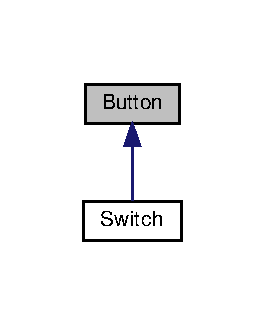
\includegraphics[width=127pt]{class_button__inherit__graph}
\end{center}
\end{figure}
\subsection*{Public Member Functions}
\begin{DoxyCompactItemize}
\item 
void \hyperlink{class_button_a5768906065b7f1d4d146f1d9fc5ce890}{init} (uint8\+\_\+t pinout\+\_\+p)
\begin{DoxyCompactList}\small\item\em Initializes the button object with given pinout. \end{DoxyCompactList}\item 
\mbox{\Hypertarget{class_button_a143f0a274b03d2bede8a84e37cd43dc7}\label{class_button_a143f0a274b03d2bede8a84e37cd43dc7}} 
bool {\bfseries is\+Pressed} ()
\end{DoxyCompactItemize}


\subsection{Detailed Description}
\hyperlink{class_button}{Button} class is responsible for reading a pushbutton state with debounce feature. \begin{Desc}
\item[Examples\+: ]\par
\hyperlink{_2home_2valentin_2_dropbox_2_a_v_i_o_n__r_c_2_prog_2_r_c_2src_2main_2control_8h-example}{/home/valentin/\+Dropbox/\+A\+V\+I\+O\+N\+\_\+\+R\+C/\+Prog/\+R\+C/src/main/control.\+h}.\end{Desc}


\subsection{Member Function Documentation}
\mbox{\Hypertarget{class_button_a5768906065b7f1d4d146f1d9fc5ce890}\label{class_button_a5768906065b7f1d4d146f1d9fc5ce890}} 
\index{Button@{Button}!init@{init}}
\index{init@{init}!Button@{Button}}
\subsubsection{\texorpdfstring{init()}{init()}}
{\footnotesize\ttfamily void Button\+::init (\begin{DoxyParamCaption}\item[{uint8\+\_\+t}]{pinout\+\_\+p }\end{DoxyParamCaption})}



Initializes the button object with given pinout. 


\begin{DoxyParams}{Parameters}
{\em pinout\+\_\+p} & the Arduino pin the button is attached to \\
\hline
\end{DoxyParams}


The documentation for this class was generated from the following files\+:\begin{DoxyCompactItemize}
\item 
src/main/\hyperlink{button_8h}{button.\+h}\item 
src/main/\hyperlink{button_8cpp}{button.\+cpp}\end{DoxyCompactItemize}

\hypertarget{class_buzzer}{}\section{Buzzer Class Reference}
\label{class_buzzer}\index{Buzzer@{Buzzer}}


\hyperlink{class_buzzer}{Buzzer} class is responsible for sound outputs.  




{\ttfamily \#include $<$buzzer.\+h$>$}

\subsection*{Public Member Functions}
\begin{DoxyCompactItemize}
\item 
void \hyperlink{class_buzzer_a55547bbb6c553f9a6f7a1d97eea4bf21}{init} (uint8\+\_\+t pinout\+\_\+p, bool enable\+\_\+p=true)
\begin{DoxyCompactList}\small\item\em Initializes buzzer on the right Arduino pin. \end{DoxyCompactList}\item 
void \hyperlink{class_buzzer_a29cb886294e260705b437dea524d43e8}{sound} (unsigned int frequency\+\_\+p, unsigned int duration\+\_\+p, unsigned int pause\+\_\+p=0)
\begin{DoxyCompactList}\small\item\em play sound \end{DoxyCompactList}\item 
\mbox{\Hypertarget{class_buzzer_a84c33234bf71806d631e1a939d649438}\label{class_buzzer_a84c33234bf71806d631e1a939d649438}} 
void {\bfseries error} ()
\item 
\mbox{\Hypertarget{class_buzzer_a9d9c6ae9bd4993d9b34a96c5ae60b5ed}\label{class_buzzer_a9d9c6ae9bd4993d9b34a96c5ae60b5ed}} 
void {\bfseries success} ()
\item 
\mbox{\Hypertarget{class_buzzer_a90e969d3ca0c6300d7639bf650cf0f79}\label{class_buzzer_a90e969d3ca0c6300d7639bf650cf0f79}} 
void {\bfseries warning} ()
\end{DoxyCompactItemize}


\subsection{Detailed Description}
\hyperlink{class_buzzer}{Buzzer} class is responsible for sound outputs. 

\subsection{Member Function Documentation}
\mbox{\Hypertarget{class_buzzer_a55547bbb6c553f9a6f7a1d97eea4bf21}\label{class_buzzer_a55547bbb6c553f9a6f7a1d97eea4bf21}} 
\index{Buzzer@{Buzzer}!init@{init}}
\index{init@{init}!Buzzer@{Buzzer}}
\subsubsection{\texorpdfstring{init()}{init()}}
{\footnotesize\ttfamily void Buzzer\+::init (\begin{DoxyParamCaption}\item[{uint8\+\_\+t}]{pinout\+\_\+p,  }\item[{bool}]{enable\+\_\+p = {\ttfamily true} }\end{DoxyParamCaption})}



Initializes buzzer on the right Arduino pin. 


\begin{DoxyParams}{Parameters}
{\em pinout\+\_\+p} & the Arduino pin the buzzer is attached to \\
\hline
{\em enable\+\_\+p} & enable or disable the buzzer (optional) \\
\hline
\end{DoxyParams}
\mbox{\Hypertarget{class_buzzer_a29cb886294e260705b437dea524d43e8}\label{class_buzzer_a29cb886294e260705b437dea524d43e8}} 
\index{Buzzer@{Buzzer}!sound@{sound}}
\index{sound@{sound}!Buzzer@{Buzzer}}
\subsubsection{\texorpdfstring{sound()}{sound()}}
{\footnotesize\ttfamily void Buzzer\+::sound (\begin{DoxyParamCaption}\item[{unsigned int}]{frequency\+\_\+p,  }\item[{unsigned int}]{duration\+\_\+p,  }\item[{unsigned int}]{pause\+\_\+p = {\ttfamily 0} }\end{DoxyParamCaption})}



play sound 


\begin{DoxyParams}{Parameters}
{\em frequency\+\_\+p} & sound frequency \\
\hline
{\em duration\+\_\+p} & sound duration \\
\hline
{\em pause\+\_\+p} & pause after sound play (optional) \\
\hline
\end{DoxyParams}


The documentation for this class was generated from the following files\+:\begin{DoxyCompactItemize}
\item 
src/main/\hyperlink{buzzer_8h}{buzzer.\+h}\item 
src/main/\hyperlink{buzzer_8cpp}{buzzer.\+cpp}\end{DoxyCompactItemize}

\hypertarget{class_control}{}\section{Control Class Reference}
\label{class_control}\index{Control@{Control}}
\subsection*{Public Member Functions}
\begin{DoxyCompactItemize}
\item 
void \hyperlink{class_control_a435c342eba3a2598f3eb40e68fa1a263}{init} (\hyperlink{class_joystick}{Joystick} left\+Joy\+\_\+p, \hyperlink{class_joystick}{Joystick} rioght\+Joy\+\_\+p, \hyperlink{class_encoder}{Encoder} encoder\+\_\+p, \hyperlink{class_switch}{Switch} gear\+Switch\+\_\+p, \hyperlink{class_buzzer}{Buzzer} buzzer\+\_\+p, \hyperlink{class_r_g_b_led}{R\+G\+B\+Led} rgb\+Led\+\_\+p, const \hyperlink{class_settings}{Settings} $\ast$p\+\_\+settings\+\_\+p)
\begin{DoxyCompactList}\small\item\em Initializes control with given joysticks. \end{DoxyCompactList}\item 
void \hyperlink{class_control_af7a1f77ddc2789d291e3193cfc046d50}{set\+Mode} (bool new\+Mode\+\_\+p)
\begin{DoxyCompactList}\small\item\em Set the Mode. \end{DoxyCompactList}\item 
\mbox{\Hypertarget{class_control_ad131914c5deeb07146127a63010480b9}\label{class_control_ad131914c5deeb07146127a63010480b9}} 
uint8\+\_\+t {\bfseries get\+Power} ()
\item 
\mbox{\Hypertarget{class_control_a3ebc07bf6326015a022e36eed5f431be}\label{class_control_a3ebc07bf6326015a022e36eed5f431be}} 
uint8\+\_\+t {\bfseries get\+Pitch} ()
\item 
\mbox{\Hypertarget{class_control_a32c3d788dfca94d73df07ef3429f222d}\label{class_control_a32c3d788dfca94d73df07ef3429f222d}} 
uint8\+\_\+t {\bfseries get\+Yaw} ()
\item 
\mbox{\Hypertarget{class_control_abf3709324d98b6dc8d52649af5d8df38}\label{class_control_abf3709324d98b6dc8d52649af5d8df38}} 
uint8\+\_\+t {\bfseries get\+Roll} ()
\end{DoxyCompactItemize}


\subsection{Detailed Description}
\begin{Desc}
\item[Examples\+: ]\par
\hyperlink{_2home_2valentin_2_dropbox_2_a_v_i_o_n__r_c_2_prog_2_r_c_2src_2main_2control_8h-example}{/home/valentin/\+Dropbox/\+A\+V\+I\+O\+N\+\_\+\+R\+C/\+Prog/\+R\+C/src/main/control.\+h}.\end{Desc}


\subsection{Member Function Documentation}
\mbox{\Hypertarget{class_control_a435c342eba3a2598f3eb40e68fa1a263}\label{class_control_a435c342eba3a2598f3eb40e68fa1a263}} 
\index{Control@{Control}!init@{init}}
\index{init@{init}!Control@{Control}}
\subsubsection{\texorpdfstring{init()}{init()}}
{\footnotesize\ttfamily void Control\+::init (\begin{DoxyParamCaption}\item[{\hyperlink{class_joystick}{Joystick}}]{left\+Joy\+\_\+p,  }\item[{\hyperlink{class_joystick}{Joystick}}]{rioght\+Joy\+\_\+p,  }\item[{\hyperlink{class_encoder}{Encoder}}]{encoder\+\_\+p,  }\item[{\hyperlink{class_switch}{Switch}}]{gear\+Switch\+\_\+p,  }\item[{\hyperlink{class_buzzer}{Buzzer}}]{buzzer\+\_\+p,  }\item[{\hyperlink{class_r_g_b_led}{R\+G\+B\+Led}}]{rgb\+Led\+\_\+p,  }\item[{const \hyperlink{class_settings}{Settings} $\ast$}]{p\+\_\+settings\+\_\+p }\end{DoxyParamCaption})}



Initializes control with given joysticks. 


\begin{DoxyParams}{Parameters}
{\em left\+Joy\+\_\+p} & left joystick object \\
\hline
{\em right\+Joy\+\_\+p} & right joystick object \\
\hline
{\em encoder\+\_\+p} & encoder objet \\
\hline
{\em gear\+Switch\+\_\+p} & switch object controlling the gear \\
\hline
{\em buzzer\+\_\+p} & buzzer object \\
\hline
{\em rgb\+Led\+\_\+p} & \hyperlink{class_r_g_b_led}{R\+G\+B\+Led} object \\
\hline
{\em p\+\_\+settings\+\_\+p} & pointer to the settings \\
\hline
\end{DoxyParams}
\begin{DoxyNote}{Note}
all objects must be initialized before 
\end{DoxyNote}
\begin{Desc}
\item[Examples\+: ]\par
\hyperlink{_2home_2valentin_2_dropbox_2_a_v_i_o_n__r_c_2_prog_2_r_c_2src_2main_2control_8h-example}{/home/valentin/\+Dropbox/\+A\+V\+I\+O\+N\+\_\+\+R\+C/\+Prog/\+R\+C/src/main/control.\+h}.\end{Desc}
\mbox{\Hypertarget{class_control_af7a1f77ddc2789d291e3193cfc046d50}\label{class_control_af7a1f77ddc2789d291e3193cfc046d50}} 
\index{Control@{Control}!set\+Mode@{set\+Mode}}
\index{set\+Mode@{set\+Mode}!Control@{Control}}
\subsubsection{\texorpdfstring{set\+Mode()}{setMode()}}
{\footnotesize\ttfamily void Control\+::set\+Mode (\begin{DoxyParamCaption}\item[{bool}]{new\+Mode\+\_\+p }\end{DoxyParamCaption})}



Set the Mode. 


\begin{DoxyParams}{Parameters}
{\em new\+Mode\+\_\+p} & new desired mode (G\+R\+O\+U\+N\+D\+\_\+\+M\+O\+DE or F\+L\+I\+G\+H\+T\+\_\+\+M\+O\+DE) \\
\hline
\end{DoxyParams}
\begin{Desc}
\item[Examples\+: ]\par
\hyperlink{_2home_2valentin_2_dropbox_2_a_v_i_o_n__r_c_2_prog_2_r_c_2src_2main_2control_8h-example}{/home/valentin/\+Dropbox/\+A\+V\+I\+O\+N\+\_\+\+R\+C/\+Prog/\+R\+C/src/main/control.\+h}.\end{Desc}


The documentation for this class was generated from the following files\+:\begin{DoxyCompactItemize}
\item 
src/main/\hyperlink{control_8h}{control.\+h}\item 
src/main/\hyperlink{control_8cpp}{control.\+cpp}\end{DoxyCompactItemize}

\hypertarget{class_encoder}{}\section{Encoder Class Reference}
\label{class_encoder}\index{Encoder@{Encoder}}


\hyperlink{class_encoder}{Encoder} class is responsible for reading rotary encoder input.  




{\ttfamily \#include $<$encoder.\+h$>$}

\subsection*{Public Member Functions}
\begin{DoxyCompactItemize}
\item 
void \hyperlink{class_encoder_a430e95a76f5b958b5350992c065d0b29}{init} (uint8\+\_\+t pinout\+A\+\_\+p, uint8\+\_\+t pinout\+B\+\_\+p, uint8\+\_\+t pinout\+S\+W\+\_\+p=-\/1)
\begin{DoxyCompactList}\small\item\em Initialize encoder pinout on Arduino board. \end{DoxyCompactList}\item 
bool \hyperlink{class_encoder_a85178b6e0978a7c342edbdce308d4abf}{refresh} ()
\begin{DoxyCompactList}\small\item\em updates encoder count after rotation \end{DoxyCompactList}\item 
int8\+\_\+t \hyperlink{class_encoder_a5e3fddf160e67d970c9c2cd57be5709a}{get\+Count} ()
\begin{DoxyCompactList}\small\item\em Get the current count. \end{DoxyCompactList}\item 
bool \hyperlink{class_encoder_ac7046bc89fc381018597bbba0cc0026e}{is\+Pressed} ()
\begin{DoxyCompactList}\small\item\em Get the current state of encoder button. \end{DoxyCompactList}\item 
\mbox{\Hypertarget{class_encoder_a8ad34a60288f78310ee465da3832b405}\label{class_encoder_a8ad34a60288f78310ee465da3832b405}} 
void \hyperlink{class_encoder_a8ad34a60288f78310ee465da3832b405}{reset} ()
\begin{DoxyCompactList}\small\item\em set m\+\_\+count to 0 \end{DoxyCompactList}\end{DoxyCompactItemize}


\subsection{Detailed Description}
\hyperlink{class_encoder}{Encoder} class is responsible for reading rotary encoder input. \begin{Desc}
\item[Examples\+: ]\par
\hyperlink{_2home_2valentin_2_dropbox_2_a_v_i_o_n__r_c_2_prog_2_r_c_2src_2main_2control_8h-example}{/home/valentin/\+Dropbox/\+A\+V\+I\+O\+N\+\_\+\+R\+C/\+Prog/\+R\+C/src/main/control.\+h}.\end{Desc}


\subsection{Member Function Documentation}
\mbox{\Hypertarget{class_encoder_a5e3fddf160e67d970c9c2cd57be5709a}\label{class_encoder_a5e3fddf160e67d970c9c2cd57be5709a}} 
\index{Encoder@{Encoder}!get\+Count@{get\+Count}}
\index{get\+Count@{get\+Count}!Encoder@{Encoder}}
\subsubsection{\texorpdfstring{get\+Count()}{getCount()}}
{\footnotesize\ttfamily int8\+\_\+t Encoder\+::get\+Count (\begin{DoxyParamCaption}{ }\end{DoxyParamCaption})}



Get the current count. 

\begin{DoxyReturn}{Returns}
int8\+\_\+t current count 
\end{DoxyReturn}
\mbox{\Hypertarget{class_encoder_a430e95a76f5b958b5350992c065d0b29}\label{class_encoder_a430e95a76f5b958b5350992c065d0b29}} 
\index{Encoder@{Encoder}!init@{init}}
\index{init@{init}!Encoder@{Encoder}}
\subsubsection{\texorpdfstring{init()}{init()}}
{\footnotesize\ttfamily void Encoder\+::init (\begin{DoxyParamCaption}\item[{uint8\+\_\+t}]{pinout\+A\+\_\+p,  }\item[{uint8\+\_\+t}]{pinout\+B\+\_\+p,  }\item[{uint8\+\_\+t}]{pinout\+S\+W\+\_\+p = {\ttfamily -\/1} }\end{DoxyParamCaption})}



Initialize encoder pinout on Arduino board. 


\begin{DoxyParams}{Parameters}
{\em pinout\+A\+\_\+p} & Arduino pin the A channel of the encoder is attached to \\
\hline
{\em pinout\+B\+\_\+p} & Arduino pin the B channel of the encoder is attached to \\
\hline
{\em pinout\+S\+W\+\_\+p} & Arduino pin the switch input of the encoder is attached to \\
\hline
\end{DoxyParams}
\mbox{\Hypertarget{class_encoder_ac7046bc89fc381018597bbba0cc0026e}\label{class_encoder_ac7046bc89fc381018597bbba0cc0026e}} 
\index{Encoder@{Encoder}!is\+Pressed@{is\+Pressed}}
\index{is\+Pressed@{is\+Pressed}!Encoder@{Encoder}}
\subsubsection{\texorpdfstring{is\+Pressed()}{isPressed()}}
{\footnotesize\ttfamily bool Encoder\+::is\+Pressed (\begin{DoxyParamCaption}{ }\end{DoxyParamCaption})}



Get the current state of encoder button. 

\begin{DoxyReturn}{Returns}
true if the rotary encoder is clicked 
\end{DoxyReturn}
\mbox{\Hypertarget{class_encoder_a85178b6e0978a7c342edbdce308d4abf}\label{class_encoder_a85178b6e0978a7c342edbdce308d4abf}} 
\index{Encoder@{Encoder}!refresh@{refresh}}
\index{refresh@{refresh}!Encoder@{Encoder}}
\subsubsection{\texorpdfstring{refresh()}{refresh()}}
{\footnotesize\ttfamily bool Encoder\+::refresh (\begin{DoxyParamCaption}{ }\end{DoxyParamCaption})}



updates encoder count after rotation 

\begin{DoxyReturn}{Returns}
true if the encoder has been rotated 
\end{DoxyReturn}


The documentation for this class was generated from the following files\+:\begin{DoxyCompactItemize}
\item 
src/main/\hyperlink{encoder_8h}{encoder.\+h}\item 
src/main/\hyperlink{encoder_8cpp}{encoder.\+cpp}\end{DoxyCompactItemize}

\hypertarget{class_joystick}{}\section{Joystick Class Reference}
\label{class_joystick}\index{Joystick@{Joystick}}


\hyperlink{class_joystick}{Joystick} class is responsible for reading joystick inputs on both axis and embedded switch.  




{\ttfamily \#include $<$joystick.\+h$>$}

\subsection*{Public Member Functions}
\begin{DoxyCompactItemize}
\item 
\mbox{\Hypertarget{class_joystick_add56a0e9f92176c9f12e3f12e3983588}\label{class_joystick_add56a0e9f92176c9f12e3f12e3983588}} 
void {\bfseries init} (uint8\+\_\+t pinout\+X\+\_\+p, uint8\+\_\+t pinout\+Y\+\_\+p, uint8\+\_\+t pinout\+S\+W\+\_\+p)
\item 
void \hyperlink{class_joystick_a70f101e3395a939fb757522b14d830c9}{set\+Idle\+Positions} (uint8\+\_\+t x\+Idle\+Position\+\_\+p, uint8\+\_\+t m\+\_\+y\+Idle\+Position\+\_\+p)
\begin{DoxyCompactList}\small\item\em Set joystick new idle positions. \end{DoxyCompactList}\item 
void \hyperlink{class_joystick_ae2a8edfcf0aa98fba3e4bfb31ebc8200}{calibrate} ()
\begin{DoxyCompactList}\small\item\em Automatically set idle positions. \end{DoxyCompactList}\item 
\mbox{\Hypertarget{class_joystick_a9f5a1ee24e763f47f60759ce35054d92}\label{class_joystick_a9f5a1ee24e763f47f60759ce35054d92}} 
uint8\+\_\+t {\bfseries readX} (bool rectify\+\_\+p=true)
\item 
\mbox{\Hypertarget{class_joystick_a53dd4c36d46f475c330ef570e62640a7}\label{class_joystick_a53dd4c36d46f475c330ef570e62640a7}} 
uint8\+\_\+t {\bfseries readY} (bool rectify\+\_\+p=true)
\item 
\mbox{\Hypertarget{class_joystick_a67821faa398aede9f7303ee69e2e1348}\label{class_joystick_a67821faa398aede9f7303ee69e2e1348}} 
bool {\bfseries is\+Pressed} ()
\item 
\mbox{\Hypertarget{class_joystick_a12b4e2601b66e1607c77c52364e96adc}\label{class_joystick_a12b4e2601b66e1607c77c52364e96adc}} 
bool {\bfseries x\+Idle} ()
\item 
\mbox{\Hypertarget{class_joystick_a02261229db91dab161af9744cc6ff81d}\label{class_joystick_a02261229db91dab161af9744cc6ff81d}} 
bool {\bfseries y\+Idle} ()
\item 
\mbox{\Hypertarget{class_joystick_af385438f23a6ed41ad3942ea1f9bf605}\label{class_joystick_af385438f23a6ed41ad3942ea1f9bf605}} 
uint8\+\_\+t {\bfseries position} ()
\item 
\mbox{\Hypertarget{class_joystick_a5a2f4443f0b0e44f328bea0137e023dd}\label{class_joystick_a5a2f4443f0b0e44f328bea0137e023dd}} 
bool {\bfseries idle} ()
\item 
\mbox{\Hypertarget{class_joystick_afd789cfd5832facccafa3784c8016b16}\label{class_joystick_afd789cfd5832facccafa3784c8016b16}} 
void {\bfseries print} ()
\end{DoxyCompactItemize}


\subsection{Detailed Description}
\hyperlink{class_joystick}{Joystick} class is responsible for reading joystick inputs on both axis and embedded switch. \begin{Desc}
\item[Examples\+: ]\par
\hyperlink{_2home_2valentin_2_dropbox_2_a_v_i_o_n__r_c_2_prog_2_r_c_2src_2main_2control_8h-example}{/home/valentin/\+Dropbox/\+A\+V\+I\+O\+N\+\_\+\+R\+C/\+Prog/\+R\+C/src/main/control.\+h}.\end{Desc}


\subsection{Member Function Documentation}
\mbox{\Hypertarget{class_joystick_ae2a8edfcf0aa98fba3e4bfb31ebc8200}\label{class_joystick_ae2a8edfcf0aa98fba3e4bfb31ebc8200}} 
\index{Joystick@{Joystick}!calibrate@{calibrate}}
\index{calibrate@{calibrate}!Joystick@{Joystick}}
\subsubsection{\texorpdfstring{calibrate()}{calibrate()}}
{\footnotesize\ttfamily void Joystick\+::calibrate (\begin{DoxyParamCaption}{ }\end{DoxyParamCaption})}



Automatically set idle positions. 

\begin{DoxyNote}{Note}
joystick must be released during the calibration process 
\end{DoxyNote}
\mbox{\Hypertarget{class_joystick_a70f101e3395a939fb757522b14d830c9}\label{class_joystick_a70f101e3395a939fb757522b14d830c9}} 
\index{Joystick@{Joystick}!set\+Idle\+Positions@{set\+Idle\+Positions}}
\index{set\+Idle\+Positions@{set\+Idle\+Positions}!Joystick@{Joystick}}
\subsubsection{\texorpdfstring{set\+Idle\+Positions()}{setIdlePositions()}}
{\footnotesize\ttfamily void Joystick\+::set\+Idle\+Positions (\begin{DoxyParamCaption}\item[{uint8\+\_\+t}]{x\+Idle\+Position\+\_\+p,  }\item[{uint8\+\_\+t}]{m\+\_\+y\+Idle\+Position\+\_\+p }\end{DoxyParamCaption})}



Set joystick new idle positions. 


\begin{DoxyParams}{Parameters}
{\em x\+Idle\+Position\+\_\+p} & x axis idle position \\
\hline
{\em y\+Idle\+Position\+\_\+p} & y axis idle position \\
\hline
\end{DoxyParams}


The documentation for this class was generated from the following files\+:\begin{DoxyCompactItemize}
\item 
src/main/\hyperlink{joystick_8h}{joystick.\+h}\item 
src/main/\hyperlink{joystick_8cpp}{joystick.\+cpp}\end{DoxyCompactItemize}

\hypertarget{class_l_c_d_screen}{}\section{L\+C\+D\+Screen Class Reference}
\label{class_l_c_d_screen}\index{L\+C\+D\+Screen@{L\+C\+D\+Screen}}


\hyperlink{class_l_c_d_screen}{L\+C\+D\+Screen} class is responsible for displaying informations on an S\+S\+D1306 I2C screen.  




{\ttfamily \#include $<$lcdscreen.\+h$>$}



Inheritance diagram for L\+C\+D\+Screen\+:\nopagebreak
\begin{figure}[H]
\begin{center}
\leavevmode
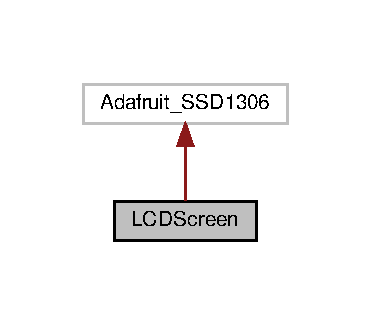
\includegraphics[width=178pt]{class_l_c_d_screen__inherit__graph}
\end{center}
\end{figure}


Collaboration diagram for L\+C\+D\+Screen\+:\nopagebreak
\begin{figure}[H]
\begin{center}
\leavevmode
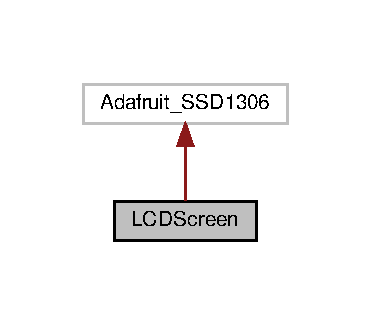
\includegraphics[width=178pt]{class_l_c_d_screen__coll__graph}
\end{center}
\end{figure}
\subsection*{Public Member Functions}
\begin{DoxyCompactItemize}
\item 
void \hyperlink{class_l_c_d_screen_af0c80235093457010a949bf1b649b919}{init} (uint8\+\_\+t display\+I2c\+Address\+\_\+p)
\begin{DoxyCompactList}\small\item\em Initialize the I2C screen. \end{DoxyCompactList}\item 
\mbox{\Hypertarget{class_l_c_d_screen_a5e55c4d461d3f19f8864c6d5c9ca2ff4}\label{class_l_c_d_screen_a5e55c4d461d3f19f8864c6d5c9ca2ff4}} 
void \hyperlink{class_l_c_d_screen_a5e55c4d461d3f19f8864c6d5c9ca2ff4}{startup} ()
\begin{DoxyCompactList}\small\item\em prints startup screen \end{DoxyCompactList}\item 
\mbox{\Hypertarget{class_l_c_d_screen_af5a86cbd7d28162e607ae15c6c5c7a2c}\label{class_l_c_d_screen_af5a86cbd7d28162e607ae15c6c5c7a2c}} 
void {\bfseries test} ()
\end{DoxyCompactItemize}


\subsection{Detailed Description}
\hyperlink{class_l_c_d_screen}{L\+C\+D\+Screen} class is responsible for displaying informations on an S\+S\+D1306 I2C screen. 

\subsection{Member Function Documentation}
\mbox{\Hypertarget{class_l_c_d_screen_af0c80235093457010a949bf1b649b919}\label{class_l_c_d_screen_af0c80235093457010a949bf1b649b919}} 
\index{L\+C\+D\+Screen@{L\+C\+D\+Screen}!init@{init}}
\index{init@{init}!L\+C\+D\+Screen@{L\+C\+D\+Screen}}
\subsubsection{\texorpdfstring{init()}{init()}}
{\footnotesize\ttfamily void L\+C\+D\+Screen\+::init (\begin{DoxyParamCaption}\item[{uint8\+\_\+t}]{display\+I2c\+Address\+\_\+p }\end{DoxyParamCaption})}



Initialize the I2C screen. 


\begin{DoxyParams}{Parameters}
{\em display\+I2c\+Address\+\_\+p} & the I2C address of the screen (can be found with examples/find\+\_\+i2c\+\_\+address/find\+\_\+i2c\+\_\+address.\+ino) \\
\hline
\end{DoxyParams}


The documentation for this class was generated from the following files\+:\begin{DoxyCompactItemize}
\item 
src/main/\hyperlink{lcdscreen_8h}{lcdscreen.\+h}\item 
src/main/\hyperlink{lcdscreen_8cpp}{lcdscreen.\+cpp}\end{DoxyCompactItemize}

\hypertarget{class_led}{}\section{Led Class Reference}
\label{class_led}\index{Led@{Led}}


\hyperlink{class_led}{Led} class is responsible for managing an electro-\/lumiscent diode output.  




{\ttfamily \#include $<$led.\+h$>$}

\subsection*{Public Member Functions}
\begin{DoxyCompactItemize}
\item 
void \hyperlink{class_led_a4bce8445a80436df1126471f83b0fb17}{init} (uint8\+\_\+t pinout\+\_\+p)
\begin{DoxyCompactList}\small\item\em Initialize the L\+ED pinout. \end{DoxyCompactList}\item 
void \hyperlink{class_led_a9136de456f7df8e202e880312767a566}{set\+State} (bool new\+State\+\_\+p)
\begin{DoxyCompactList}\small\item\em Set the State. \end{DoxyCompactList}\item 
bool \hyperlink{class_led_a3c98242eb57df713fcb8d441d43ccd02}{get\+State} ()
\begin{DoxyCompactList}\small\item\em Get the current state of the L\+ED. \end{DoxyCompactList}\item 
\mbox{\Hypertarget{class_led_a02561ef42927779f247c0ae714a89e9a}\label{class_led_a02561ef42927779f247c0ae714a89e9a}} 
void \hyperlink{class_led_a02561ef42927779f247c0ae714a89e9a}{turn\+On} ()
\begin{DoxyCompactList}\small\item\em turns the L\+ED on \end{DoxyCompactList}\item 
\mbox{\Hypertarget{class_led_a3c581311221a0fedafdfb250a1f318ab}\label{class_led_a3c581311221a0fedafdfb250a1f318ab}} 
void \hyperlink{class_led_a3c581311221a0fedafdfb250a1f318ab}{turn\+Off} ()
\begin{DoxyCompactList}\small\item\em turns the L\+ED off \end{DoxyCompactList}\item 
void \hyperlink{class_led_a5ffc6040a68800545f1d063641cad66d}{blink} (int period\+\_\+p, int duration\+\_\+p=1)
\begin{DoxyCompactList}\small\item\em blinks the L\+ED \end{DoxyCompactList}\end{DoxyCompactItemize}


\subsection{Detailed Description}
\hyperlink{class_led}{Led} class is responsible for managing an electro-\/lumiscent diode output. 

\subsection{Member Function Documentation}
\mbox{\Hypertarget{class_led_a5ffc6040a68800545f1d063641cad66d}\label{class_led_a5ffc6040a68800545f1d063641cad66d}} 
\index{Led@{Led}!blink@{blink}}
\index{blink@{blink}!Led@{Led}}
\subsubsection{\texorpdfstring{blink()}{blink()}}
{\footnotesize\ttfamily void Led\+::blink (\begin{DoxyParamCaption}\item[{int}]{period\+\_\+p,  }\item[{int}]{duration\+\_\+p = {\ttfamily 1} }\end{DoxyParamCaption})}



blinks the L\+ED 

\begin{DoxyNote}{Note}
blocking method 
\end{DoxyNote}

\begin{DoxyParams}{Parameters}
{\em period\+\_\+p} & blink period (in milliseconds) \\
\hline
{\em duration\+\_\+p} & number of blinks \\
\hline
\end{DoxyParams}
\mbox{\Hypertarget{class_led_a3c98242eb57df713fcb8d441d43ccd02}\label{class_led_a3c98242eb57df713fcb8d441d43ccd02}} 
\index{Led@{Led}!get\+State@{get\+State}}
\index{get\+State@{get\+State}!Led@{Led}}
\subsubsection{\texorpdfstring{get\+State()}{getState()}}
{\footnotesize\ttfamily bool Led\+::get\+State (\begin{DoxyParamCaption}{ }\end{DoxyParamCaption})}



Get the current state of the L\+ED. 

\begin{DoxyReturn}{Returns}
m\+\_\+led\+State 
\end{DoxyReturn}
\mbox{\Hypertarget{class_led_a4bce8445a80436df1126471f83b0fb17}\label{class_led_a4bce8445a80436df1126471f83b0fb17}} 
\index{Led@{Led}!init@{init}}
\index{init@{init}!Led@{Led}}
\subsubsection{\texorpdfstring{init()}{init()}}
{\footnotesize\ttfamily void Led\+::init (\begin{DoxyParamCaption}\item[{uint8\+\_\+t}]{pinout\+\_\+p }\end{DoxyParamCaption})}



Initialize the L\+ED pinout. 


\begin{DoxyParams}{Parameters}
{\em pinout\+\_\+p} & the Arduino pin the L\+ED is attached to \\
\hline
\end{DoxyParams}
\mbox{\Hypertarget{class_led_a9136de456f7df8e202e880312767a566}\label{class_led_a9136de456f7df8e202e880312767a566}} 
\index{Led@{Led}!set\+State@{set\+State}}
\index{set\+State@{set\+State}!Led@{Led}}
\subsubsection{\texorpdfstring{set\+State()}{setState()}}
{\footnotesize\ttfamily void Led\+::set\+State (\begin{DoxyParamCaption}\item[{bool}]{new\+State\+\_\+p }\end{DoxyParamCaption})}



Set the State. 


\begin{DoxyParams}{Parameters}
{\em new\+State\+\_\+p} & \\
\hline
\end{DoxyParams}


The documentation for this class was generated from the following files\+:\begin{DoxyCompactItemize}
\item 
src/main/\hyperlink{led_8h}{led.\+h}\item 
src/main/\hyperlink{led_8cpp}{led.\+cpp}\end{DoxyCompactItemize}

\hypertarget{class_plane_battery_bisplay}{}\section{Plane\+Battery\+Bisplay Class Reference}
\label{class_plane_battery_bisplay}\index{Plane\+Battery\+Bisplay@{Plane\+Battery\+Bisplay}}
\subsection*{Public Member Functions}
\begin{DoxyCompactItemize}
\item 
\mbox{\Hypertarget{class_plane_battery_bisplay_a2e5a1c0a536c707a2d02562210fa8d67}\label{class_plane_battery_bisplay_a2e5a1c0a536c707a2d02562210fa8d67}} 
void {\bfseries print\+Cell} (uint8\+\_\+t cell\+Select\+\_\+p)
\item 
\mbox{\Hypertarget{class_plane_battery_bisplay_ae3c48c207bc32d8b76b7d5790574de60}\label{class_plane_battery_bisplay_ae3c48c207bc32d8b76b7d5790574de60}} 
void {\bfseries print\+Next\+Cell} ()
\end{DoxyCompactItemize}


The documentation for this class was generated from the following files\+:\begin{DoxyCompactItemize}
\item 
src/main/plane\+\_\+battery\+\_\+display.\+h\item 
src/main/plane\+\_\+battery\+\_\+display.\+cpp\end{DoxyCompactItemize}

\hypertarget{struct_pto_t_data_frame}{}\section{Pto\+T\+Data\+Frame Struct Reference}
\label{struct_pto_t_data_frame}\index{Pto\+T\+Data\+Frame@{Pto\+T\+Data\+Frame}}


Struct composed with all data contained in a frame sent from the Plane to the Transmitter.  




{\ttfamily \#include $<$frame.\+h$>$}

\subsection*{Public Attributes}
\begin{DoxyCompactItemize}
\item 
\mbox{\Hypertarget{struct_pto_t_data_frame_a06150f36a41a099e881ddd9f7b49d7d5}\label{struct_pto_t_data_frame_a06150f36a41a099e881ddd9f7b49d7d5}} 
float {\bfseries cell\+Voltages} \mbox{[}L\+I\+P\+O\+\_\+2S\mbox{]}
\item 
\mbox{\Hypertarget{struct_pto_t_data_frame_ae47149352f0c6871a0d814b374df741e}\label{struct_pto_t_data_frame_ae47149352f0c6871a0d814b374df741e}} 
float {\bfseries temp}
\item 
\mbox{\Hypertarget{struct_pto_t_data_frame_a57d2dbacceafb000649f3a1beb865acc}\label{struct_pto_t_data_frame_a57d2dbacceafb000649f3a1beb865acc}} 
float {\bfseries hum}
\end{DoxyCompactItemize}


\subsection{Detailed Description}
Struct composed with all data contained in a frame sent from the Plane to the Transmitter. 

The documentation for this struct was generated from the following file\+:\begin{DoxyCompactItemize}
\item 
src/main/\hyperlink{frame_8h}{frame.\+h}\end{DoxyCompactItemize}

\hypertarget{class_radio}{}\section{Radio Class Reference}
\label{class_radio}\index{Radio@{Radio}}


\hyperlink{class_radio}{Radio} class responsible for communicating with the \hyperlink{class_radio}{Radio} Transmitter on the ground.  




{\ttfamily \#include $<$radio.\+h$>$}



Inheritance diagram for Radio\+:
\nopagebreak
\begin{figure}[H]
\begin{center}
\leavevmode
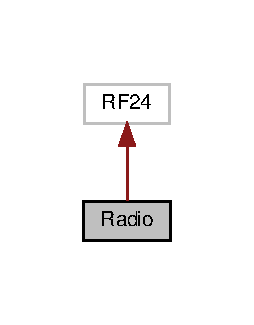
\includegraphics[width=122pt]{class_radio__inherit__graph}
\end{center}
\end{figure}


Collaboration diagram for Radio\+:
\nopagebreak
\begin{figure}[H]
\begin{center}
\leavevmode
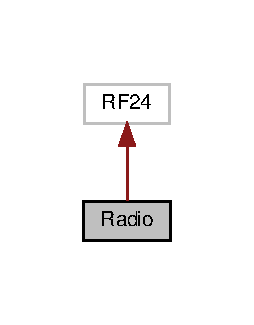
\includegraphics[width=122pt]{class_radio__coll__graph}
\end{center}
\end{figure}
\subsection*{Public Member Functions}
\begin{DoxyCompactItemize}
\item 
\mbox{\Hypertarget{class_radio_a0775d3e885563f797abf893bd7dab722}\label{class_radio_a0775d3e885563f797abf893bd7dab722}} 
{\bfseries Radio} (uint8\+\_\+t C\+Epin\+\_\+p, uint8\+\_\+t C\+Spin\+\_\+p)
\item 
\mbox{\Hypertarget{class_radio_a0824b3e73e1285a98b818a40e30eb784}\label{class_radio_a0824b3e73e1285a98b818a40e30eb784}} 
void {\bfseries init} (uint8\+\_\+t C\+Epin\+\_\+p, uint8\+\_\+t C\+Spin\+\_\+p)
\item 
bool \hyperlink{class_radio_acb313b8c4ccfbe9eed993d566e563f89}{wait\+For\+Connection} (int time\+Out\+\_\+p)
\begin{DoxyCompactList}\small\item\em wait until Transmitter handshake \end{DoxyCompactList}\item 
\mbox{\Hypertarget{class_radio_a531aebd77214bc665027819db617a81d}\label{class_radio_a531aebd77214bc665027819db617a81d}} 
bool {\bfseries is\+Connected} ()
\item 
bool \hyperlink{class_radio_a50a86b8fbc5cd906c721d54406f98b9b}{authenticate\+Remote} ()
\begin{DoxyCompactList}\small\item\em validates an authentication frame \end{DoxyCompactList}\item 
\mbox{\Hypertarget{class_radio_a85f5d3b2851f7787337c410f8608a45a}\label{class_radio_a85f5d3b2851f7787337c410f8608a45a}} 
bool {\bfseries data\+Available} ()
\item 
\mbox{\Hypertarget{class_radio_af5f2ff2feaa025d251f6ec3682fb6477}\label{class_radio_af5f2ff2feaa025d251f6ec3682fb6477}} 
bool {\bfseries receive\+Data} ()
\item 
\mbox{\Hypertarget{class_radio_a470a9f109780600f2e3ff815ff85f2f5}\label{class_radio_a470a9f109780600f2e3ff815ff85f2f5}} 
bool {\bfseries send\+Authentication\+Ack} ()
\item 
\mbox{\Hypertarget{class_radio_a666fdbfbf97b5cdd91e8a07fa9cd3fed}\label{class_radio_a666fdbfbf97b5cdd91e8a07fa9cd3fed}} 
bool {\bfseries send\+Data} ()
\item 
\mbox{\Hypertarget{class_radio_a269cbab3a0ae4e0d4e514f7ce83fe4fb}\label{class_radio_a269cbab3a0ae4e0d4e514f7ce83fe4fb}} 
uint8\+\_\+t {\bfseries get\+Roll} ()
\item 
\mbox{\Hypertarget{class_radio_a497f8533da9df3d64ca8bbe5ddb6477c}\label{class_radio_a497f8533da9df3d64ca8bbe5ddb6477c}} 
uint8\+\_\+t {\bfseries get\+Pitch} ()
\item 
\mbox{\Hypertarget{class_radio_ab5828ab85c10d920c650a44b78225563}\label{class_radio_ab5828ab85c10d920c650a44b78225563}} 
uint8\+\_\+t {\bfseries get\+Yaw} ()
\item 
\mbox{\Hypertarget{class_radio_a4060add1b24bc065f05abd969acc5573}\label{class_radio_a4060add1b24bc065f05abd969acc5573}} 
uint8\+\_\+t {\bfseries get\+Power} ()
\end{DoxyCompactItemize}


\subsection{Detailed Description}
\hyperlink{class_radio}{Radio} class responsible for communicating with the \hyperlink{class_radio}{Radio} Transmitter on the ground. 

\subsection{Member Function Documentation}
\mbox{\Hypertarget{class_radio_a50a86b8fbc5cd906c721d54406f98b9b}\label{class_radio_a50a86b8fbc5cd906c721d54406f98b9b}} 
\index{Radio@{Radio}!authenticate\+Remote@{authenticate\+Remote}}
\index{authenticate\+Remote@{authenticate\+Remote}!Radio@{Radio}}
\subsubsection{\texorpdfstring{authenticate\+Remote()}{authenticateRemote()}}
{\footnotesize\ttfamily bool Radio\+::authenticate\+Remote (\begin{DoxyParamCaption}{ }\end{DoxyParamCaption})}



validates an authentication frame 

\begin{DoxyReturn}{Returns}
true if last frame is a valid authentication frame 
\end{DoxyReturn}
\mbox{\Hypertarget{class_radio_acb313b8c4ccfbe9eed993d566e563f89}\label{class_radio_acb313b8c4ccfbe9eed993d566e563f89}} 
\index{Radio@{Radio}!wait\+For\+Connection@{wait\+For\+Connection}}
\index{wait\+For\+Connection@{wait\+For\+Connection}!Radio@{Radio}}
\subsubsection{\texorpdfstring{wait\+For\+Connection()}{waitForConnection()}}
{\footnotesize\ttfamily bool Radio\+::wait\+For\+Connection (\begin{DoxyParamCaption}\item[{int}]{time\+Out\+\_\+p = {\ttfamily -\/1} }\end{DoxyParamCaption})}



wait until Transmitter handshake 

\begin{DoxyNote}{Note}
blocking method with optional timeout 
\end{DoxyNote}

\begin{DoxyParams}{Parameters}
{\em time\+Out\+\_\+p} & optional timeout in seconds \\
\hline
\end{DoxyParams}
\begin{DoxyReturn}{Returns}
true if connection is established before timeout 
\end{DoxyReturn}


The documentation for this class was generated from the following files\+:\begin{DoxyCompactItemize}
\item 
src/main/\hyperlink{radio_8h}{radio.\+h}\item 
src/main/\hyperlink{radio_8cpp}{radio.\+cpp}\end{DoxyCompactItemize}

\hypertarget{class_remote_battery}{}\section{Remote\+Battery Class Reference}
\label{class_remote_battery}\index{Remote\+Battery@{Remote\+Battery}}


\hyperlink{class_remote_battery}{Remote\+Battery} class is responsible for managing the battery level of the plane.  




{\ttfamily \#include $<$remote\+\_\+battery.\+h$>$}



Inheritance diagram for Remote\+Battery\+:\nopagebreak
\begin{figure}[H]
\begin{center}
\leavevmode
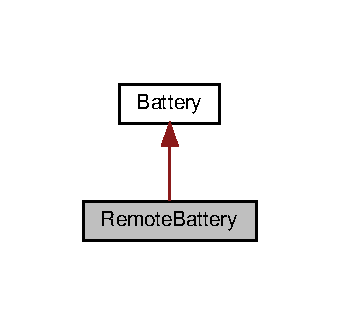
\includegraphics[width=163pt]{class_remote_battery__inherit__graph}
\end{center}
\end{figure}


Collaboration diagram for Remote\+Battery\+:\nopagebreak
\begin{figure}[H]
\begin{center}
\leavevmode
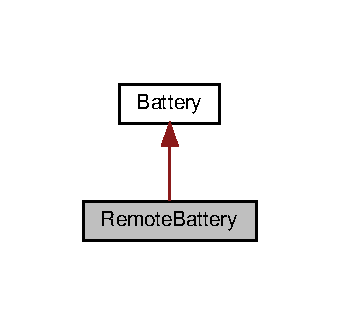
\includegraphics[width=163pt]{class_remote_battery__coll__graph}
\end{center}
\end{figure}


\subsection{Detailed Description}
\hyperlink{class_remote_battery}{Remote\+Battery} class is responsible for managing the battery level of the plane. 

The documentation for this class was generated from the following files\+:\begin{DoxyCompactItemize}
\item 
src/main/\hyperlink{remote__battery_8h}{remote\+\_\+battery.\+h}\item 
src/main/\hyperlink{remote__battery_8cpp}{remote\+\_\+battery.\+cpp}\end{DoxyCompactItemize}

\hypertarget{class_r_g_b_led}{}\section{R\+G\+B\+Led Class Reference}
\label{class_r_g_b_led}\index{R\+G\+B\+Led@{R\+G\+B\+Led}}


\hyperlink{class_r_g_b_led}{R\+G\+B\+Led} class is responsible for displaying colors on an R\+GB \hyperlink{class_led}{Led}.  




{\ttfamily \#include $<$rgbled.\+h$>$}

\subsection*{Public Member Functions}
\begin{DoxyCompactItemize}
\item 
void \hyperlink{class_r_g_b_led_aa12ca52b63da78e35b6bbec3624df991}{init} (bool led\+Type\+\_\+p, uint8\+\_\+t red\+Pin\+\_\+p, uint8\+\_\+t green\+Pin\+\_\+p, uint8\+\_\+t blue\+Pin\+\_\+p)
\begin{DoxyCompactList}\small\item\em initializes led type and pinout \end{DoxyCompactList}\item 
void \hyperlink{class_r_g_b_led_a9ab9701eb0f4d945fd9ca6e2235d7ee9}{write\+Color\+Pin} (uint8\+\_\+t color\+Pin\+\_\+p, bool new\+State\+\_\+p)
\item 
void \hyperlink{class_r_g_b_led_a6a1e12a1f48fc29acd30aa88a1cfd1b1}{display\+Color} (uint8\+\_\+t color\+\_\+p)
\begin{DoxyCompactList}\small\item\em displays a specific color \end{DoxyCompactList}\item 
\mbox{\Hypertarget{class_r_g_b_led_af00b4e0ef8ec0aea4452fc2133b03453}\label{class_r_g_b_led_af00b4e0ef8ec0aea4452fc2133b03453}} 
void {\bfseries turn\+Off} ()
\end{DoxyCompactItemize}


\subsection{Detailed Description}
\hyperlink{class_r_g_b_led}{R\+G\+B\+Led} class is responsible for displaying colors on an R\+GB \hyperlink{class_led}{Led}. 

\subsection{Member Function Documentation}
\mbox{\Hypertarget{class_r_g_b_led_a6a1e12a1f48fc29acd30aa88a1cfd1b1}\label{class_r_g_b_led_a6a1e12a1f48fc29acd30aa88a1cfd1b1}} 
\index{R\+G\+B\+Led@{R\+G\+B\+Led}!display\+Color@{display\+Color}}
\index{display\+Color@{display\+Color}!R\+G\+B\+Led@{R\+G\+B\+Led}}
\subsubsection{\texorpdfstring{display\+Color()}{displayColor()}}
{\footnotesize\ttfamily void R\+G\+B\+Led\+::display\+Color (\begin{DoxyParamCaption}\item[{uint8\+\_\+t}]{color\+\_\+p }\end{DoxyParamCaption})}



displays a specific color 


\begin{DoxyParams}{Parameters}
{\em color\+\_\+p} & \\
\hline
\end{DoxyParams}
\mbox{\Hypertarget{class_r_g_b_led_aa12ca52b63da78e35b6bbec3624df991}\label{class_r_g_b_led_aa12ca52b63da78e35b6bbec3624df991}} 
\index{R\+G\+B\+Led@{R\+G\+B\+Led}!init@{init}}
\index{init@{init}!R\+G\+B\+Led@{R\+G\+B\+Led}}
\subsubsection{\texorpdfstring{init()}{init()}}
{\footnotesize\ttfamily void R\+G\+B\+Led\+::init (\begin{DoxyParamCaption}\item[{bool}]{led\+Type\+\_\+p,  }\item[{uint8\+\_\+t}]{red\+Pin\+\_\+p,  }\item[{uint8\+\_\+t}]{green\+Pin\+\_\+p,  }\item[{uint8\+\_\+t}]{blue\+Pin\+\_\+p }\end{DoxyParamCaption})}



initializes led type and pinout 


\begin{DoxyParams}{Parameters}
{\em led\+Type\+\_\+p} & can be either R\+G\+B\+\_\+\+C\+O\+M\+M\+O\+N\+\_\+\+A\+N\+O\+DE or R\+G\+B\+\_\+\+C\+O\+M\+M\+O\+N\+\_\+\+C\+A\+T\+H\+O\+DE \\
\hline
{\em red\+Pin\+\_\+p} & the arduino pin the led red pin is connected to \\
\hline
{\em green\+Pin\+\_\+p} & the arduino pin the led green pin is connected to \\
\hline
{\em blue\+Pin\+\_\+p} & the arduino pin the led blue pin is connected to \\
\hline
\end{DoxyParams}
\mbox{\Hypertarget{class_r_g_b_led_a9ab9701eb0f4d945fd9ca6e2235d7ee9}\label{class_r_g_b_led_a9ab9701eb0f4d945fd9ca6e2235d7ee9}} 
\index{R\+G\+B\+Led@{R\+G\+B\+Led}!write\+Color\+Pin@{write\+Color\+Pin}}
\index{write\+Color\+Pin@{write\+Color\+Pin}!R\+G\+B\+Led@{R\+G\+B\+Led}}
\subsubsection{\texorpdfstring{write\+Color\+Pin()}{writeColorPin()}}
{\footnotesize\ttfamily void R\+G\+B\+Led\+::write\+Color\+Pin (\begin{DoxyParamCaption}\item[{uint8\+\_\+t}]{color\+Pin\+\_\+p,  }\item[{bool}]{new\+State\+\_\+p }\end{DoxyParamCaption})}


\begin{DoxyParams}{Parameters}
{\em color\+Pin\+\_\+p} & color selector, can be R\+ED, G\+R\+E\+EN or B\+L\+UE \\
\hline
{\em new\+State\+\_\+p} & new state, can be \\
\hline
\end{DoxyParams}


The documentation for this class was generated from the following files\+:\begin{DoxyCompactItemize}
\item 
src/main/\hyperlink{rgbled_8h}{rgbled.\+h}\item 
src/main/\hyperlink{rgbled_8cpp}{rgbled.\+cpp}\end{DoxyCompactItemize}

\hypertarget{class_settings}{}\section{Settings Class Reference}
\label{class_settings}\index{Settings@{Settings}}


\hyperlink{class_settings}{Settings} class is responsible for.  




{\ttfamily \#include $<$settings.\+h$>$}

\subsection*{Public Member Functions}
\begin{DoxyCompactItemize}
\item 
bool \hyperlink{class_settings_a513f67eb1af1a2ca93bebddfce8e1e0a}{write\+To\+Mem} (uint16\+\_\+t index\+\_\+p=-\/1)
\begin{DoxyCompactList}\small\item\em write setting(s) into E\+E\+P\+R\+OM persistent memory \end{DoxyCompactList}\item 
{\footnotesize template$<$typename T $>$ }\\T \hyperlink{class_settings_a49f0ce2f4dbff5b59f4b8658a06b49bb}{read\+From\+Mem} (uint16\+\_\+t index\+\_\+p=-\/1, bool update\+Settings\+\_\+p=true)
\begin{DoxyCompactList}\small\item\em reads data from E\+E\+P\+R\+OM persistent memory \end{DoxyCompactList}\item 
{\footnotesize template$<$typename T $>$ }\\void \hyperlink{class_settings_ab5a7de6e9d4f0b59d9cf93957e33cf49}{set\+Setting} (uint8\+\_\+t index\+\_\+p, T new\+Value\+\_\+p, bool write\+To\+Mem\+\_\+p=false)
\begin{DoxyCompactList}\small\item\em Set a bool Setting value. \end{DoxyCompactList}\item 
{\footnotesize template$<$typename T $>$ }\\const T \hyperlink{class_settings_a61df1edd21940600c4c6647adb177a91}{get\+Setting} (uint8\+\_\+t index\+\_\+p) const
\begin{DoxyCompactList}\small\item\em Get the Setting value. \end{DoxyCompactList}\end{DoxyCompactItemize}


\subsection{Detailed Description}
\hyperlink{class_settings}{Settings} class is responsible for. \begin{Desc}
\item[Examples\+: ]\par
\hyperlink{_2home_2valentin_2_dropbox_2_a_v_i_o_n__r_c_2_prog_2_r_c_2src_2main_2control_8h-example}{/home/valentin/\+Dropbox/\+A\+V\+I\+O\+N\+\_\+\+R\+C/\+Prog/\+R\+C/src/main/control.\+h}.\end{Desc}


\subsection{Member Function Documentation}
\mbox{\Hypertarget{class_settings_a61df1edd21940600c4c6647adb177a91}\label{class_settings_a61df1edd21940600c4c6647adb177a91}} 
\index{Settings@{Settings}!get\+Setting@{get\+Setting}}
\index{get\+Setting@{get\+Setting}!Settings@{Settings}}
\subsubsection{\texorpdfstring{get\+Setting()}{getSetting()}}
{\footnotesize\ttfamily template$<$typename T $>$ \\
const T Settings\+::get\+Setting (\begin{DoxyParamCaption}\item[{uint8\+\_\+t}]{index\+\_\+p }\end{DoxyParamCaption}) const\hspace{0.3cm}{\ttfamily [inline]}}



Get the Setting value. 


\begin{DoxyTemplParams}{Template Parameters}
{\em T} & type of setting \\
\hline
\end{DoxyTemplParams}

\begin{DoxyParams}{Parameters}
{\em index\+\_\+p} & index of setting \\
\hline
\end{DoxyParams}
\begin{DoxyReturn}{Returns}

\end{DoxyReturn}
\mbox{\Hypertarget{class_settings_a49f0ce2f4dbff5b59f4b8658a06b49bb}\label{class_settings_a49f0ce2f4dbff5b59f4b8658a06b49bb}} 
\index{Settings@{Settings}!read\+From\+Mem@{read\+From\+Mem}}
\index{read\+From\+Mem@{read\+From\+Mem}!Settings@{Settings}}
\subsubsection{\texorpdfstring{read\+From\+Mem()}{readFromMem()}}
{\footnotesize\ttfamily template$<$typename T $>$ \\
T Settings\+::read\+From\+Mem (\begin{DoxyParamCaption}\item[{uint16\+\_\+t}]{index\+\_\+p = {\ttfamily -\/1},  }\item[{bool}]{update\+Settings\+\_\+p = {\ttfamily true} }\end{DoxyParamCaption})\hspace{0.3cm}{\ttfamily [inline]}}



reads data from E\+E\+P\+R\+OM persistent memory 


\begin{DoxyTemplParams}{Template Parameters}
{\em T} & type of data to read \\
\hline
\end{DoxyTemplParams}

\begin{DoxyParams}{Parameters}
{\em index\+\_\+p} & (optional) \\
\hline
{\em update\+Settings\+\_\+p} & set to true to update class member \\
\hline
\end{DoxyParams}
\begin{DoxyNote}{Note}
if no index\+\_\+p is passed, the method will read all settings and return the first one 
\end{DoxyNote}
\begin{DoxyReturn}{Returns}
T 
\end{DoxyReturn}
\mbox{\Hypertarget{class_settings_ab5a7de6e9d4f0b59d9cf93957e33cf49}\label{class_settings_ab5a7de6e9d4f0b59d9cf93957e33cf49}} 
\index{Settings@{Settings}!set\+Setting@{set\+Setting}}
\index{set\+Setting@{set\+Setting}!Settings@{Settings}}
\subsubsection{\texorpdfstring{set\+Setting()}{setSetting()}}
{\footnotesize\ttfamily template$<$typename T $>$ \\
void Settings\+::set\+Setting (\begin{DoxyParamCaption}\item[{uint8\+\_\+t}]{index\+\_\+p,  }\item[{T}]{new\+Value\+\_\+p,  }\item[{bool}]{write\+To\+Mem\+\_\+p = {\ttfamily false} }\end{DoxyParamCaption})\hspace{0.3cm}{\ttfamily [inline]}}



Set a bool Setting value. 


\begin{DoxyTemplParams}{Template Parameters}
{\em T} & type of setting value \\
\hline
\end{DoxyTemplParams}

\begin{DoxyParams}{Parameters}
{\em index\+\_\+p} & index of setting \\
\hline
{\em new\+Value\+\_\+p} & new setting value \\
\hline
{\em write\+To\+Mem\+\_\+p} & true to immediately update value in E\+E\+P\+R\+OM persistent memory (if necessary) \\
\hline
\end{DoxyParams}
\mbox{\Hypertarget{class_settings_a513f67eb1af1a2ca93bebddfce8e1e0a}\label{class_settings_a513f67eb1af1a2ca93bebddfce8e1e0a}} 
\index{Settings@{Settings}!write\+To\+Mem@{write\+To\+Mem}}
\index{write\+To\+Mem@{write\+To\+Mem}!Settings@{Settings}}
\subsubsection{\texorpdfstring{write\+To\+Mem()}{writeToMem()}}
{\footnotesize\ttfamily bool Settings\+::write\+To\+Mem (\begin{DoxyParamCaption}\item[{uint16\+\_\+t}]{index\+\_\+p = {\ttfamily -\/1} }\end{DoxyParamCaption})\hspace{0.3cm}{\ttfamily [inline]}}



write setting(s) into E\+E\+P\+R\+OM persistent memory 


\begin{DoxyParams}{Parameters}
{\em index\+\_\+p} & index of setting to write \\
\hline
\end{DoxyParams}
\begin{DoxyNote}{Note}
if index\+\_\+p is undefined, all settings will be written in E\+E\+P\+R\+OM 

since each byte of arduino E\+E\+P\+R\+OM is limited to approx. 100000 writings, limit usage of this method to the strict minimum 
\end{DoxyNote}
\begin{DoxyReturn}{Returns}
true if write operation was necessary 
\end{DoxyReturn}


The documentation for this class was generated from the following files\+:\begin{DoxyCompactItemize}
\item 
src/main/\hyperlink{settings_8h}{settings.\+h}\item 
src/main/\hyperlink{settings_8cpp}{settings.\+cpp}\end{DoxyCompactItemize}

\hypertarget{class_sevseg_screen}{}\section{Sevseg\+Screen Class Reference}
\label{class_sevseg_screen}\index{Sevseg\+Screen@{Sevseg\+Screen}}


\hyperlink{class_sevseg_screen}{Sevseg\+Screen} class is responsible for displaying content on a 7-\/segment display.  




{\ttfamily \#include $<$sevsegscreen.\+h$>$}



Inheritance diagram for Sevseg\+Screen\+:\nopagebreak
\begin{figure}[H]
\begin{center}
\leavevmode
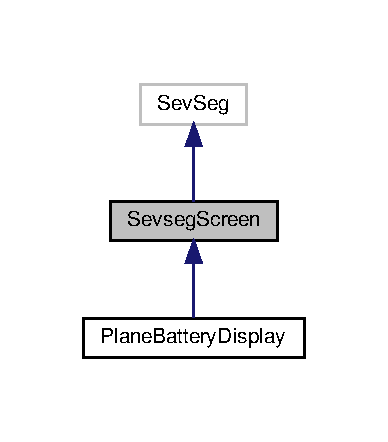
\includegraphics[width=185pt]{class_sevseg_screen__inherit__graph}
\end{center}
\end{figure}


Collaboration diagram for Sevseg\+Screen\+:\nopagebreak
\begin{figure}[H]
\begin{center}
\leavevmode
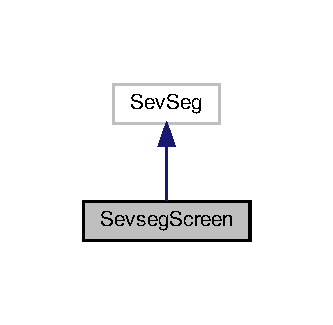
\includegraphics[width=160pt]{class_sevseg_screen__coll__graph}
\end{center}
\end{figure}
\subsection*{Public Member Functions}
\begin{DoxyCompactItemize}
\item 
void \hyperlink{class_sevseg_screen_a29e517dc7ddda7547fe8f7c706654444}{init} (bool display\+Type\+\_\+p, uint8\+\_\+t nb\+Digits\+\_\+p, uint8\+\_\+t $\ast$sev\+Seg\+Digits\+Pinout\+\_\+p, uint8\+\_\+t $\ast$sev\+Seg\+Segments\+Pinout\+\_\+p)
\begin{DoxyCompactList}\small\item\em Initializes display pinout. \end{DoxyCompactList}\item 
void \hyperlink{class_sevseg_screen_a3afbaf812d953f552b6d0e80de61804e}{chrono} ()
\begin{DoxyCompactList}\small\item\em test the display with a simple chronometer \end{DoxyCompactList}\item 
void \hyperlink{class_sevseg_screen_ad82130595693d5f18c81c1ca5206da15}{test\+Display} ()
\begin{DoxyCompactList}\small\item\em test display by printing rotating pattern on all digits \end{DoxyCompactList}\end{DoxyCompactItemize}


\subsection{Detailed Description}
\hyperlink{class_sevseg_screen}{Sevseg\+Screen} class is responsible for displaying content on a 7-\/segment display. 

\subsection{Member Function Documentation}
\mbox{\Hypertarget{class_sevseg_screen_a3afbaf812d953f552b6d0e80de61804e}\label{class_sevseg_screen_a3afbaf812d953f552b6d0e80de61804e}} 
\index{Sevseg\+Screen@{Sevseg\+Screen}!chrono@{chrono}}
\index{chrono@{chrono}!Sevseg\+Screen@{Sevseg\+Screen}}
\subsubsection{\texorpdfstring{chrono()}{chrono()}}
{\footnotesize\ttfamily void Sevseg\+Screen\+::chrono (\begin{DoxyParamCaption}{ }\end{DoxyParamCaption})}



test the display with a simple chronometer 

\begin{DoxyNote}{Note}
this function must be called in a while(true) loop 
\end{DoxyNote}
\mbox{\Hypertarget{class_sevseg_screen_a29e517dc7ddda7547fe8f7c706654444}\label{class_sevseg_screen_a29e517dc7ddda7547fe8f7c706654444}} 
\index{Sevseg\+Screen@{Sevseg\+Screen}!init@{init}}
\index{init@{init}!Sevseg\+Screen@{Sevseg\+Screen}}
\subsubsection{\texorpdfstring{init()}{init()}}
{\footnotesize\ttfamily void Sevseg\+Screen\+::init (\begin{DoxyParamCaption}\item[{bool}]{display\+Type\+\_\+p,  }\item[{uint8\+\_\+t}]{nb\+Digits\+\_\+p,  }\item[{uint8\+\_\+t $\ast$}]{sev\+Seg\+Digits\+Pinout\+\_\+p,  }\item[{uint8\+\_\+t $\ast$}]{sev\+Seg\+Segments\+Pinout\+\_\+p }\end{DoxyParamCaption})}



Initializes display pinout. 


\begin{DoxyParams}{Parameters}
{\em display\+Type\+\_\+p} & type of display, can be either C\+O\+M\+M\+O\+N\+\_\+\+A\+N\+D\+OE or C\+O\+M\+M\+O\+N\+\_\+\+C\+A\+T\+H\+O\+DE \\
\hline
{\em nb\+Digits\+\_\+p} & numbre of digits of the display \\
\hline
{\em sev\+Seg\+Digits\+Pinout\+\_\+p} & pinout of display segments in the order \{A,B,C,D,E,F,G,DP\} \\
\hline
{\em sev\+Seg\+Segments\+Pinout\+\_\+p} & pinout of the display digits \\
\hline
\end{DoxyParams}
\mbox{\Hypertarget{class_sevseg_screen_ad82130595693d5f18c81c1ca5206da15}\label{class_sevseg_screen_ad82130595693d5f18c81c1ca5206da15}} 
\index{Sevseg\+Screen@{Sevseg\+Screen}!test\+Display@{test\+Display}}
\index{test\+Display@{test\+Display}!Sevseg\+Screen@{Sevseg\+Screen}}
\subsubsection{\texorpdfstring{test\+Display()}{testDisplay()}}
{\footnotesize\ttfamily void Sevseg\+Screen\+::test\+Display (\begin{DoxyParamCaption}{ }\end{DoxyParamCaption})}



test display by printing rotating pattern on all digits 

\begin{DoxyNote}{Note}
blocking method 
\end{DoxyNote}


The documentation for this class was generated from the following files\+:\begin{DoxyCompactItemize}
\item 
src/main/\hyperlink{sevsegscreen_8h}{sevsegscreen.\+h}\item 
src/main/\hyperlink{sevsegscreen_8cpp}{sevsegscreen.\+cpp}\end{DoxyCompactItemize}

\hypertarget{class_switch}{}\section{Switch Class Reference}
\label{class_switch}\index{Switch@{Switch}}


\hyperlink{class_switch}{Switch} class is responsible for managing a 2-\/positions switch input.  




{\ttfamily \#include $<$switch.\+h$>$}



Inheritance diagram for Switch\+:\nopagebreak
\begin{figure}[H]
\begin{center}
\leavevmode
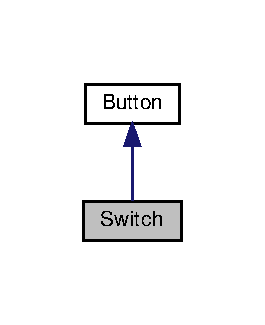
\includegraphics[width=127pt]{class_switch__inherit__graph}
\end{center}
\end{figure}


Collaboration diagram for Switch\+:\nopagebreak
\begin{figure}[H]
\begin{center}
\leavevmode
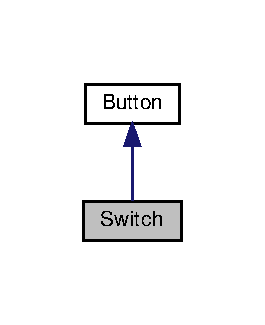
\includegraphics[width=127pt]{class_switch__coll__graph}
\end{center}
\end{figure}
\subsection*{Public Member Functions}
\begin{DoxyCompactItemize}
\item 
bool \hyperlink{class_switch_ac9b4369bd630f9d975f2bd82933f7cc6}{state} ()
\begin{DoxyCompactList}\small\item\em read switch current state \end{DoxyCompactList}\end{DoxyCompactItemize}


\subsection{Detailed Description}
\hyperlink{class_switch}{Switch} class is responsible for managing a 2-\/positions switch input. \begin{Desc}
\item[Examples\+: ]\par
\hyperlink{_2home_2valentin_2_dropbox_2_a_v_i_o_n__r_c_2_prog_2_r_c_2src_2main_2control_8h-example}{/home/valentin/\+Dropbox/\+A\+V\+I\+O\+N\+\_\+\+R\+C/\+Prog/\+R\+C/src/main/control.\+h}.\end{Desc}


\subsection{Member Function Documentation}
\mbox{\Hypertarget{class_switch_ac9b4369bd630f9d975f2bd82933f7cc6}\label{class_switch_ac9b4369bd630f9d975f2bd82933f7cc6}} 
\index{Switch@{Switch}!state@{state}}
\index{state@{state}!Switch@{Switch}}
\subsubsection{\texorpdfstring{state()}{state()}}
{\footnotesize\ttfamily bool Switch\+::state (\begin{DoxyParamCaption}{ }\end{DoxyParamCaption})}



read switch current state 

\begin{DoxyReturn}{Returns}
true if the switch is on 
\end{DoxyReturn}


The documentation for this class was generated from the following files\+:\begin{DoxyCompactItemize}
\item 
src/main/\hyperlink{switch_8h}{switch.\+h}\item 
src/main/switch.\+cpp\end{DoxyCompactItemize}

\hypertarget{struct_tto_p_data_frame}{}\section{Tto\+P\+Data\+Frame Struct Reference}
\label{struct_tto_p_data_frame}\index{Tto\+P\+Data\+Frame@{Tto\+P\+Data\+Frame}}


Struct composed with all data contained in a frame sent from the Transmitter to the Plane.  




{\ttfamily \#include $<$frame.\+h$>$}

\subsection*{Public Attributes}
\begin{DoxyCompactItemize}
\item 
\mbox{\Hypertarget{struct_tto_p_data_frame_a3bbd087f4b60b7394a603ae3b6a97823}\label{struct_tto_p_data_frame_a3bbd087f4b60b7394a603ae3b6a97823}} 
uint8\+\_\+t {\bfseries roll}
\item 
\mbox{\Hypertarget{struct_tto_p_data_frame_a97d0b21d8d48f84e459735aea087338c}\label{struct_tto_p_data_frame_a97d0b21d8d48f84e459735aea087338c}} 
uint8\+\_\+t {\bfseries pitch}
\item 
\mbox{\Hypertarget{struct_tto_p_data_frame_a006555f9f0b70c2253dd38ca78917a84}\label{struct_tto_p_data_frame_a006555f9f0b70c2253dd38ca78917a84}} 
uint8\+\_\+t {\bfseries yaw}
\item 
\mbox{\Hypertarget{struct_tto_p_data_frame_a49a1f4d925f15a0de6244c5a89607089}\label{struct_tto_p_data_frame_a49a1f4d925f15a0de6244c5a89607089}} 
uint8\+\_\+t {\bfseries power}
\end{DoxyCompactItemize}


\subsection{Detailed Description}
Struct composed with all data contained in a frame sent from the Transmitter to the Plane. 

The documentation for this struct was generated from the following file\+:\begin{DoxyCompactItemize}
\item 
src/main/\hyperlink{frame_8h}{frame.\+h}\end{DoxyCompactItemize}

\chapter{File Documentation}
\hypertarget{battery_8cpp}{}\section{src/main/battery.cpp File Reference}
\label{battery_8cpp}\index{src/main/battery.\+cpp@{src/main/battery.\+cpp}}


definition of battery class  


{\ttfamily \#include \char`\"{}battery.\+h\char`\"{}}\newline
{\ttfamily \#include $<$Arduino.\+h$>$}\newline
Include dependency graph for battery.\+cpp\+:\nopagebreak
\begin{figure}[H]
\begin{center}
\leavevmode
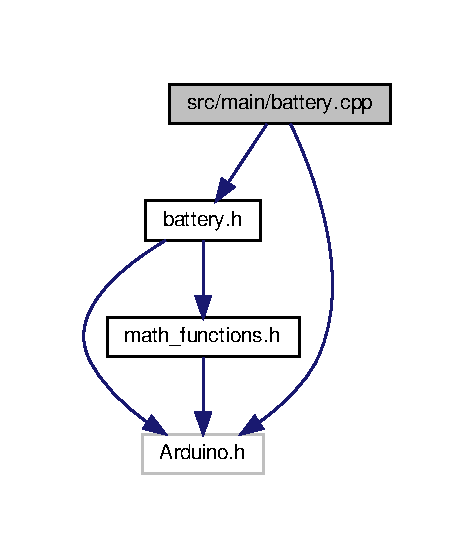
\includegraphics[width=225pt]{battery_8cpp__incl}
\end{center}
\end{figure}
\subsection*{Functions}
\begin{DoxyCompactItemize}
\item 
\mbox{\Hypertarget{battery_8cpp_a2f439a0487cb7a0c584cc43a4e72c7ac}\label{battery_8cpp_a2f439a0487cb7a0c584cc43a4e72c7ac}} 
float {\bfseries map\+Float} (float base, float min\+Base, float max\+Base, float new\+Min, float new\+Max)
\end{DoxyCompactItemize}


\subsection{Detailed Description}
definition of battery class 

\begin{DoxyAuthor}{Author}
Valentin Mercy (\href{https://github.com/vmercy}{\tt https\+://github.\+com/vmercy}) 
\end{DoxyAuthor}
\begin{DoxyVersion}{Version}
0.\+1 
\end{DoxyVersion}
\begin{DoxyDate}{Date}
2020-\/11-\/23
\end{DoxyDate}
\begin{DoxyCopyright}{Copyright}
Copyright (c) 2020 
\end{DoxyCopyright}

\hypertarget{battery_8h}{}\section{src/main/battery.h File Reference}
\label{battery_8h}\index{src/main/battery.\+h@{src/main/battery.\+h}}


declaration of battery class  


{\ttfamily \#include $<$Arduino.\+h$>$}\newline
{\ttfamily \#include \char`\"{}math\+\_\+functions.\+h\char`\"{}}\newline
Include dependency graph for battery.\+h\+:\nopagebreak
\begin{figure}[H]
\begin{center}
\leavevmode
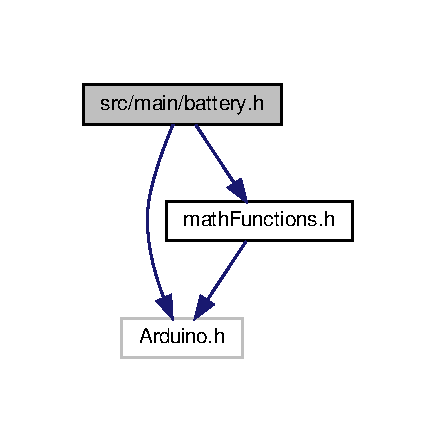
\includegraphics[width=211pt]{battery_8h__incl}
\end{center}
\end{figure}
This graph shows which files directly or indirectly include this file\+:\nopagebreak
\begin{figure}[H]
\begin{center}
\leavevmode
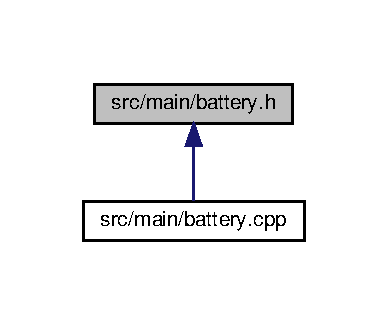
\includegraphics[width=298pt]{battery_8h__dep__incl}
\end{center}
\end{figure}
\subsection*{Classes}
\begin{DoxyCompactItemize}
\item 
class \hyperlink{class_battery}{Battery}
\end{DoxyCompactItemize}
\subsection*{Macros}
\begin{DoxyCompactItemize}
\item 
\mbox{\Hypertarget{battery_8h_af81c563d212b04612a2fdf09f5b2957c}\label{battery_8h_af81c563d212b04612a2fdf09f5b2957c}} 
\#define {\bfseries L\+I\+P\+O\+\_\+1S}~1
\item 
\mbox{\Hypertarget{battery_8h_a0ff9eb1042b121287d6abfe776ec1a8c}\label{battery_8h_a0ff9eb1042b121287d6abfe776ec1a8c}} 
\#define {\bfseries L\+I\+P\+O\+\_\+2S}~2
\item 
\mbox{\Hypertarget{battery_8h_a194fd11d79140854ebb63b4aae64f105}\label{battery_8h_a194fd11d79140854ebb63b4aae64f105}} 
\#define {\bfseries L\+I\+P\+O\+\_\+3S}~3
\item 
\mbox{\Hypertarget{battery_8h_adb9cf7290df946a808d907fd52b36adf}\label{battery_8h_adb9cf7290df946a808d907fd52b36adf}} 
\#define {\bfseries L\+I\+P\+O\+\_\+4S}~4
\item 
\mbox{\Hypertarget{battery_8h_a96a8f65f4f6e996672b62adfe98d7c46}\label{battery_8h_a96a8f65f4f6e996672b62adfe98d7c46}} 
\#define {\bfseries L\+I\+P\+O\+\_\+5S}~5
\item 
\mbox{\Hypertarget{battery_8h_a62ca371673d32217c9314773078b55ee}\label{battery_8h_a62ca371673d32217c9314773078b55ee}} 
\#define {\bfseries L\+I\+P\+O\+\_\+6S}~6
\item 
\mbox{\Hypertarget{battery_8h_ad5ec179af884bf5d81f7d7d277ad72d0}\label{battery_8h_ad5ec179af884bf5d81f7d7d277ad72d0}} 
\#define {\bfseries L\+I\+P\+O\+\_\+\+L\+O\+W\+E\+S\+T\+\_\+\+V\+O\+L\+T\+A\+GE}~3.\+3
\item 
\mbox{\Hypertarget{battery_8h_a01732358c09897aadb81cf1e07a73eca}\label{battery_8h_a01732358c09897aadb81cf1e07a73eca}} 
\#define {\bfseries L\+I\+P\+O\+\_\+\+H\+I\+G\+H\+E\+S\+T\+\_\+\+V\+O\+L\+T\+A\+GE}~4.\+2
\item 
\mbox{\Hypertarget{battery_8h_a65d999b485fd49b24b03c98367813603}\label{battery_8h_a65d999b485fd49b24b03c98367813603}} 
\#define {\bfseries B\+A\+T\+T\+E\+R\+Y\+\_\+\+C\+E\+L\+L\+\_\+\+A\+L\+E\+R\+T\+\_\+\+V\+O\+L\+T\+A\+GE}~3.\+5
\item 
\mbox{\Hypertarget{battery_8h_a3d0dbddf2f4fe415ee4c5bf20d12dc37}\label{battery_8h_a3d0dbddf2f4fe415ee4c5bf20d12dc37}} 
\#define {\bfseries B\+A\+T\+T\+E\+R\+Y\+\_\+\+C\+E\+L\+L\+\_\+\+C\+R\+I\+T\+I\+C\+A\+L\+\_\+\+V\+O\+L\+T\+A\+GE}~3.\+4
\item 
\mbox{\Hypertarget{battery_8h_af5eb7e3dc57a2c282b06f32e51970839}\label{battery_8h_af5eb7e3dc57a2c282b06f32e51970839}} 
\#define {\bfseries A\+N\+A\+L\+O\+G\+\_\+\+R\+EF}~5.\+0
\item 
\mbox{\Hypertarget{battery_8h_a38b266fc2a691a397cb0739a9e19c0a1}\label{battery_8h_a38b266fc2a691a397cb0739a9e19c0a1}} 
\#define {\bfseries A\+N\+A\+L\+O\+G\+\_\+\+P\+R\+E\+C\+I\+S\+I\+ON}~1023
\item 
\mbox{\Hypertarget{battery_8h_a2674a2c5313fff69210125ef15558bf7}\label{battery_8h_a2674a2c5313fff69210125ef15558bf7}} 
\#define {\bfseries N\+B\+\_\+\+S\+A\+M\+P\+L\+E\+S\+\_\+\+B\+A\+T\+T\+E\+RY}~10
\item 
\mbox{\Hypertarget{battery_8h_a33fa689903e4d19edd814aa108d49a91}\label{battery_8h_a33fa689903e4d19edd814aa108d49a91}} 
\#define {\bfseries D\+E\+L\+A\+Y\+\_\+\+S\+A\+M\+P\+L\+E\+S\+\_\+\+B\+A\+T\+T\+E\+RY}~500
\end{DoxyCompactItemize}


\subsection{Detailed Description}
declaration of battery class 

\begin{DoxyAuthor}{Author}
Valentin Mercy (\href{https://github.com/vmercy}{\tt https\+://github.\+com/vmercy}) 
\end{DoxyAuthor}
\begin{DoxyVersion}{Version}
0.\+1 
\end{DoxyVersion}
\begin{DoxyDate}{Date}
2020-\/11-\/21
\end{DoxyDate}
\begin{DoxyCopyright}{Copyright}
Copyright (c) 2020 
\end{DoxyCopyright}

\hypertarget{button_8cpp}{}\section{src/main/button.cpp File Reference}
\label{button_8cpp}\index{src/main/button.\+cpp@{src/main/button.\+cpp}}


Definition of \hyperlink{class_button}{Button} class.  


{\ttfamily \#include \char`\"{}button.\+h\char`\"{}}\newline
Include dependency graph for button.\+cpp\+:
\nopagebreak
\begin{figure}[H]
\begin{center}
\leavevmode
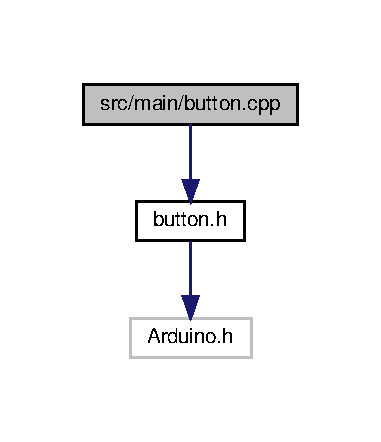
\includegraphics[width=183pt]{button_8cpp__incl}
\end{center}
\end{figure}


\subsection{Detailed Description}
Definition of \hyperlink{class_button}{Button} class. 

\begin{DoxyAuthor}{Author}
Valentin Mercy (\href{https://github.com/vmercy}{\tt https\+://github.\+com/vmercy}) 
\end{DoxyAuthor}
\begin{DoxyVersion}{Version}
0.\+1 
\end{DoxyVersion}
\begin{DoxyDate}{Date}
2020-\/11-\/26
\end{DoxyDate}
\begin{DoxyCopyright}{Copyright}
Copyright (c) 2020 
\end{DoxyCopyright}

\hypertarget{button_8h}{}\section{src/main/button.h File Reference}
\label{button_8h}\index{src/main/button.\+h@{src/main/button.\+h}}


Declaration of \hyperlink{class_button}{Button} class.  


{\ttfamily \#include $<$Arduino.\+h$>$}\newline
Include dependency graph for button.\+h\+:\nopagebreak
\begin{figure}[H]
\begin{center}
\leavevmode
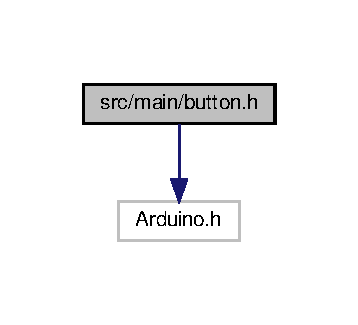
\includegraphics[width=172pt]{button_8h__incl}
\end{center}
\end{figure}
This graph shows which files directly or indirectly include this file\+:\nopagebreak
\begin{figure}[H]
\begin{center}
\leavevmode
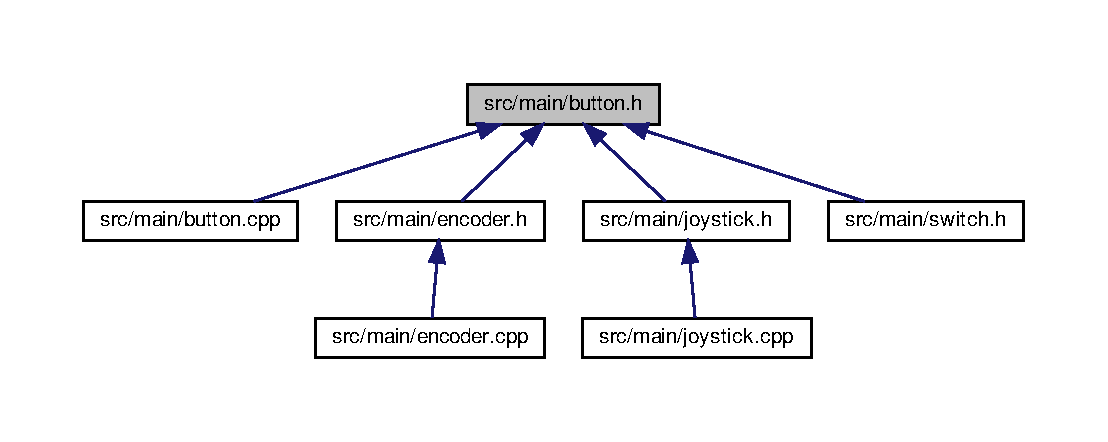
\includegraphics[width=350pt]{button_8h__dep__incl}
\end{center}
\end{figure}
\subsection*{Classes}
\begin{DoxyCompactItemize}
\item 
class \hyperlink{class_button}{Button}
\begin{DoxyCompactList}\small\item\em \hyperlink{class_button}{Button} class is responsible for reading a pushbutton state with debounce feature. \end{DoxyCompactList}\end{DoxyCompactItemize}
\subsection*{Macros}
\begin{DoxyCompactItemize}
\item 
\mbox{\Hypertarget{button_8h_adb75862f582a7d68347ceae4f4c003c9}\label{button_8h_adb75862f582a7d68347ceae4f4c003c9}} 
\#define {\bfseries D\+E\+B\+O\+U\+N\+C\+E\+\_\+\+D\+E\+L\+AY}~2
\end{DoxyCompactItemize}


\subsection{Detailed Description}
Declaration of \hyperlink{class_button}{Button} class. 

\begin{DoxyAuthor}{Author}
Valentin Mercy (\href{https://github.com/vmercy}{\tt https\+://github.\+com/vmercy}) 
\end{DoxyAuthor}
\begin{DoxyVersion}{Version}
0.\+1 
\end{DoxyVersion}
\begin{DoxyDate}{Date}
2020-\/11-\/26
\end{DoxyDate}
\begin{DoxyCopyright}{Copyright}
Copyright (c) 2020 
\end{DoxyCopyright}

\hypertarget{buzzer_8cpp}{}\section{src/main/buzzer.cpp File Reference}
\label{buzzer_8cpp}\index{src/main/buzzer.\+cpp@{src/main/buzzer.\+cpp}}


Definition of buzzer class.  


{\ttfamily \#include \char`\"{}buzzer.\+h\char`\"{}}\newline
Include dependency graph for buzzer.\+cpp\+:
\nopagebreak
\begin{figure}[H]
\begin{center}
\leavevmode
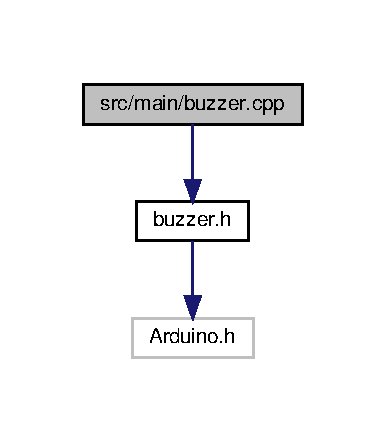
\includegraphics[width=185pt]{buzzer_8cpp__incl}
\end{center}
\end{figure}


\subsection{Detailed Description}
Definition of buzzer class. 

\begin{DoxyAuthor}{Author}
Valentin Mercy (\href{https://github.com/vmercy}{\tt https\+://github.\+com/vmercy}) 
\end{DoxyAuthor}
\begin{DoxyVersion}{Version}
0.\+1 
\end{DoxyVersion}
\begin{DoxyDate}{Date}
2020-\/11-\/27
\end{DoxyDate}
\begin{DoxyCopyright}{Copyright}
Copyright (c) 2020 
\end{DoxyCopyright}

\hypertarget{buzzer_8h}{}\section{src/main/buzzer.h File Reference}
\label{buzzer_8h}\index{src/main/buzzer.\+h@{src/main/buzzer.\+h}}


Declaration of \hyperlink{class_buzzer}{Buzzer} class.  


{\ttfamily \#include $<$Arduino.\+h$>$}\newline
Include dependency graph for buzzer.\+h\+:\nopagebreak
\begin{figure}[H]
\begin{center}
\leavevmode
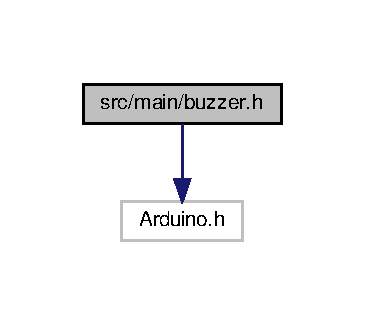
\includegraphics[width=175pt]{buzzer_8h__incl}
\end{center}
\end{figure}
This graph shows which files directly or indirectly include this file\+:\nopagebreak
\begin{figure}[H]
\begin{center}
\leavevmode
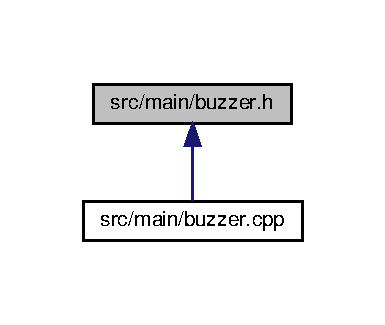
\includegraphics[width=303pt]{buzzer_8h__dep__incl}
\end{center}
\end{figure}
\subsection*{Classes}
\begin{DoxyCompactItemize}
\item 
class \hyperlink{class_buzzer}{Buzzer}
\begin{DoxyCompactList}\small\item\em \hyperlink{class_buzzer}{Buzzer} class is responsible for sound outputs. \end{DoxyCompactList}\end{DoxyCompactItemize}


\subsection{Detailed Description}
Declaration of \hyperlink{class_buzzer}{Buzzer} class. 

\begin{DoxyAuthor}{Author}
Valentin Mercy (\href{https://github.com/vmercy}{\tt https\+://github.\+com/vmercy}) 
\end{DoxyAuthor}
\begin{DoxyVersion}{Version}
0.\+1 
\end{DoxyVersion}
\begin{DoxyDate}{Date}
2020-\/11-\/27
\end{DoxyDate}
\begin{DoxyCopyright}{Copyright}
Copyright (c) 2020 
\end{DoxyCopyright}

\hypertarget{control_8cpp}{}\section{src/main/control.cpp File Reference}
\label{control_8cpp}\index{src/main/control.\+cpp@{src/main/control.\+cpp}}


Definition of control class.  


{\ttfamily \#include \char`\"{}control.\+h\char`\"{}}\newline
Include dependency graph for control.\+cpp\+:\nopagebreak
\begin{figure}[H]
\begin{center}
\leavevmode
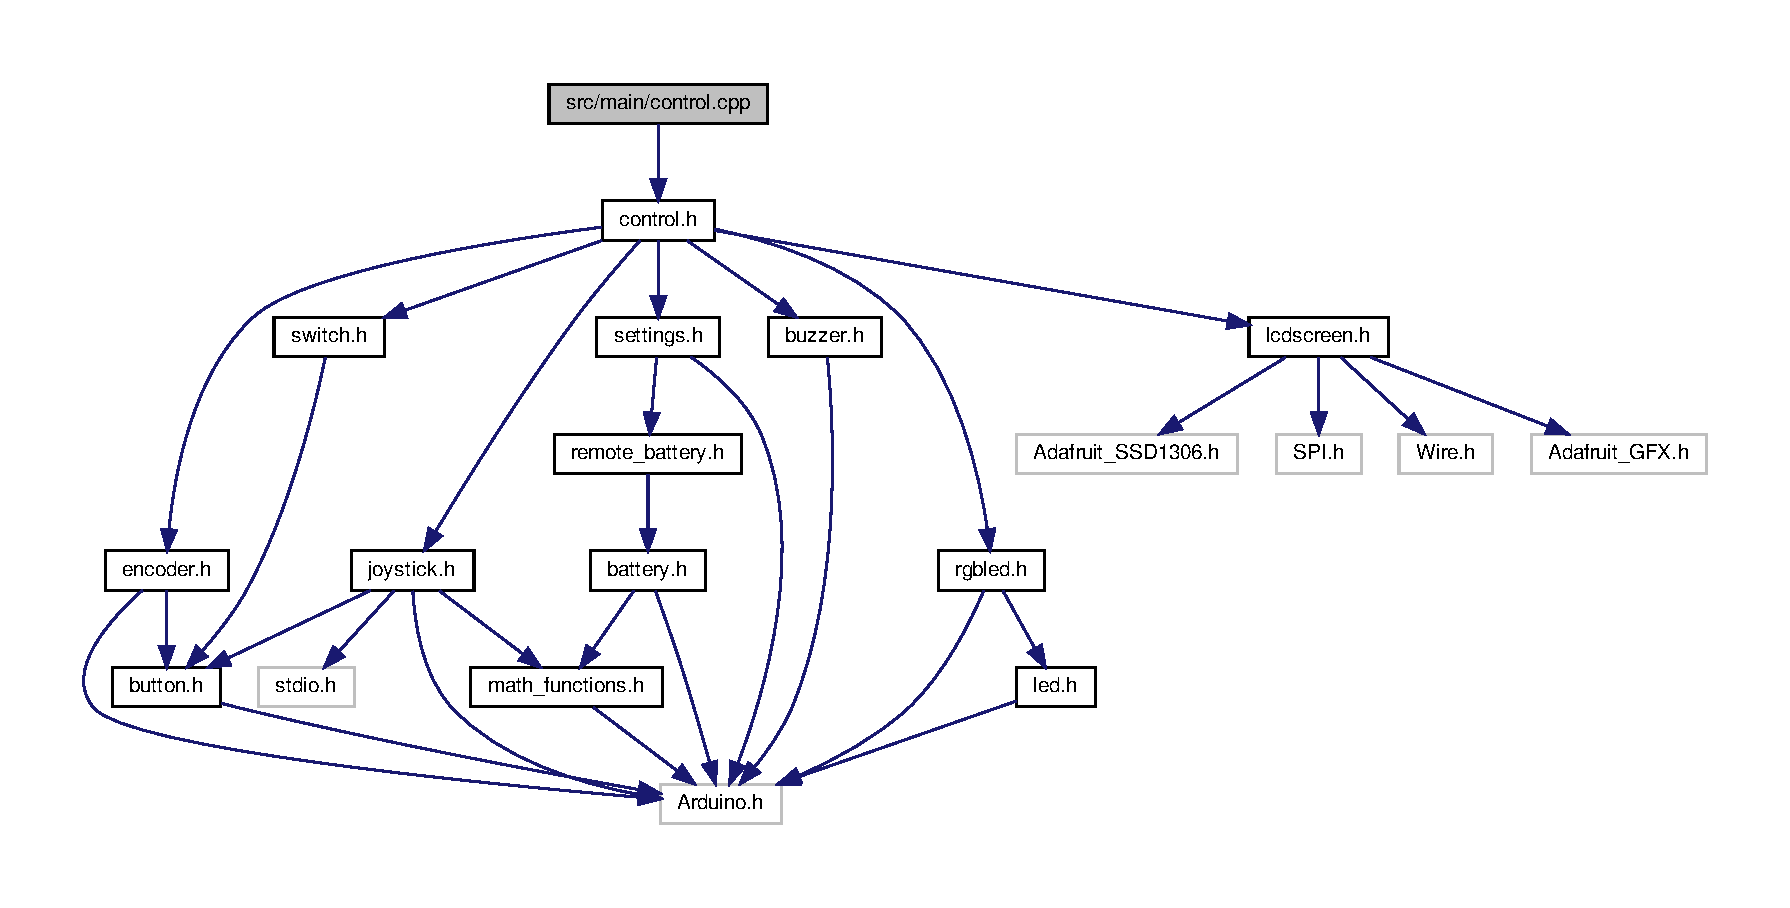
\includegraphics[width=350pt]{control_8cpp__incl}
\end{center}
\end{figure}


\subsection{Detailed Description}
Definition of control class. 

\begin{DoxyAuthor}{Author}
Valentin Mercy (\href{https://github.com/vmercy}{\tt https\+://github.\+com/vmercy}) 
\end{DoxyAuthor}
\begin{DoxyVersion}{Version}
0.\+1 
\end{DoxyVersion}
\begin{DoxyDate}{Date}
2020-\/12-\/21 
\end{DoxyDate}
\begin{DoxyCopyright}{Copyright}
Copyright (c) 2020 
\end{DoxyCopyright}

\hypertarget{control_8h}{}\section{src/main/control.h File Reference}
\label{control_8h}\index{src/main/control.\+h@{src/main/control.\+h}}


Declaration of control class.  


{\ttfamily \#include \char`\"{}joystick.\+h\char`\"{}}\newline
{\ttfamily \#include \char`\"{}encoder.\+h\char`\"{}}\newline
{\ttfamily \#include \char`\"{}buzzer.\+h\char`\"{}}\newline
{\ttfamily \#include \char`\"{}rgbled.\+h\char`\"{}}\newline
{\ttfamily \#include \char`\"{}switch.\+h\char`\"{}}\newline
{\ttfamily \#include \char`\"{}lcdscreen.\+h\char`\"{}}\newline
{\ttfamily \#include \char`\"{}settings.\+h\char`\"{}}\newline
Include dependency graph for control.\+h\+:\nopagebreak
\begin{figure}[H]
\begin{center}
\leavevmode
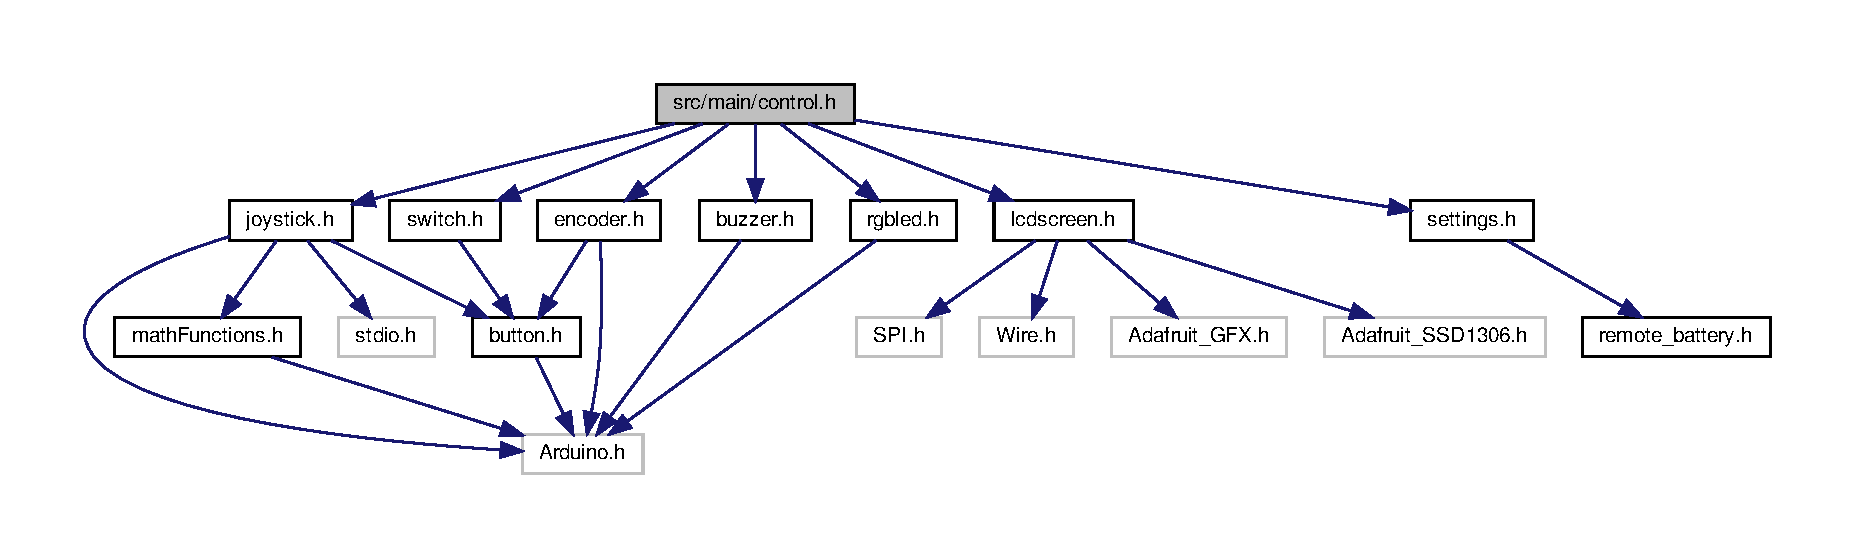
\includegraphics[width=350pt]{control_8h__incl}
\end{center}
\end{figure}
This graph shows which files directly or indirectly include this file\+:\nopagebreak
\begin{figure}[H]
\begin{center}
\leavevmode
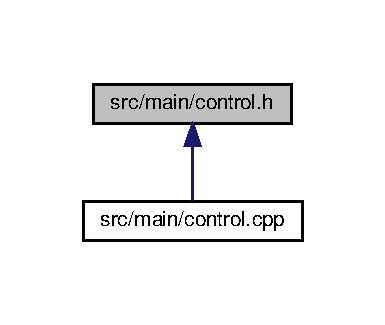
\includegraphics[width=185pt]{control_8h__dep__incl}
\end{center}
\end{figure}
\subsection*{Classes}
\begin{DoxyCompactItemize}
\item 
class \hyperlink{class_control}{Control}
\end{DoxyCompactItemize}
\subsection*{Macros}
\begin{DoxyCompactItemize}
\item 
\mbox{\Hypertarget{control_8h_a3518fb2d38b90114c5bacca8b3ad5fcb}\label{control_8h_a3518fb2d38b90114c5bacca8b3ad5fcb}} 
\#define {\bfseries G\+R\+O\+U\+N\+D\+\_\+\+M\+O\+DE}~0
\item 
\mbox{\Hypertarget{control_8h_a80bbd95a50bfb90e017945a610e39837}\label{control_8h_a80bbd95a50bfb90e017945a610e39837}} 
\#define {\bfseries F\+L\+I\+G\+H\+T\+\_\+\+M\+O\+DE}~1
\item 
\mbox{\Hypertarget{control_8h_a5a10849857f3344ba3aef3bf81bb53aa}\label{control_8h_a5a10849857f3344ba3aef3bf81bb53aa}} 
\#define {\bfseries C\+O\+N\+T\+R\+O\+L\+\_\+\+I\+D\+LE}~128
\end{DoxyCompactItemize}


\subsection{Detailed Description}
Declaration of control class. 

\begin{DoxyAuthor}{Author}
Valentin Mercy (\href{https://github.com/vmercy}{\tt https\+://github.\+com/vmercy}) 
\end{DoxyAuthor}
\begin{DoxyVersion}{Version}
0.\+1 
\end{DoxyVersion}
\begin{DoxyDate}{Date}
2020-\/12-\/21
\end{DoxyDate}
\begin{DoxyCopyright}{Copyright}
Copyright (c) 2020 
\end{DoxyCopyright}

\hypertarget{encoder_8cpp}{}\section{src/main/encoder.cpp File Reference}
\label{encoder_8cpp}\index{src/main/encoder.\+cpp@{src/main/encoder.\+cpp}}


Definition of \hyperlink{class_encoder}{Encoder} class.  


{\ttfamily \#include \char`\"{}encoder.\+h\char`\"{}}\newline
Include dependency graph for encoder.\+cpp\+:
\nopagebreak
\begin{figure}[H]
\begin{center}
\leavevmode
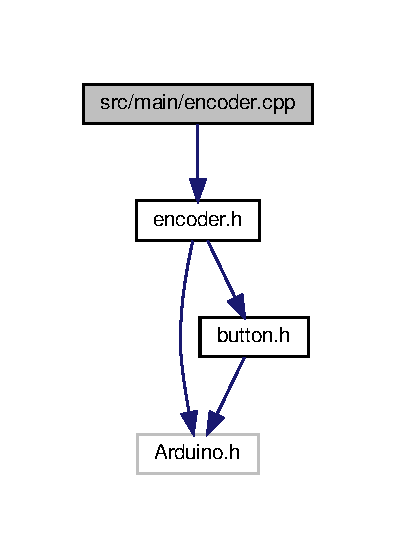
\includegraphics[width=190pt]{encoder_8cpp__incl}
\end{center}
\end{figure}


\subsection{Detailed Description}
Definition of \hyperlink{class_encoder}{Encoder} class. 

\begin{DoxyAuthor}{Author}
Valentin Mercy (\href{https://github.com/vmercy}{\tt https\+://github.\+com/vmercy}) 
\end{DoxyAuthor}
\begin{DoxyVersion}{Version}
0.\+1 
\end{DoxyVersion}
\begin{DoxyDate}{Date}
2020-\/11-\/27
\end{DoxyDate}
\begin{DoxyCopyright}{Copyright}
Copyright (c) 2020 
\end{DoxyCopyright}

\hypertarget{encoder_8h}{}\section{src/main/encoder.h File Reference}
\label{encoder_8h}\index{src/main/encoder.\+h@{src/main/encoder.\+h}}


Declaration of \hyperlink{class_encoder}{Encoder} class.  


{\ttfamily \#include $<$Arduino.\+h$>$}\newline
{\ttfamily \#include \char`\"{}button.\+h\char`\"{}}\newline
Include dependency graph for encoder.\+h\+:\nopagebreak
\begin{figure}[H]
\begin{center}
\leavevmode
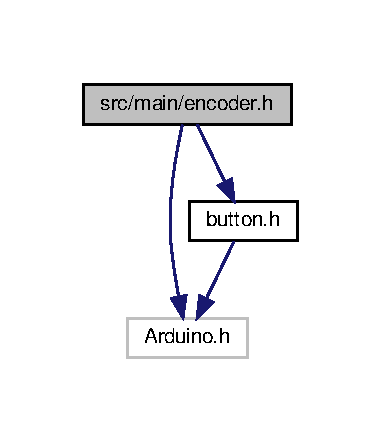
\includegraphics[width=183pt]{encoder_8h__incl}
\end{center}
\end{figure}
This graph shows which files directly or indirectly include this file\+:\nopagebreak
\begin{figure}[H]
\begin{center}
\leavevmode
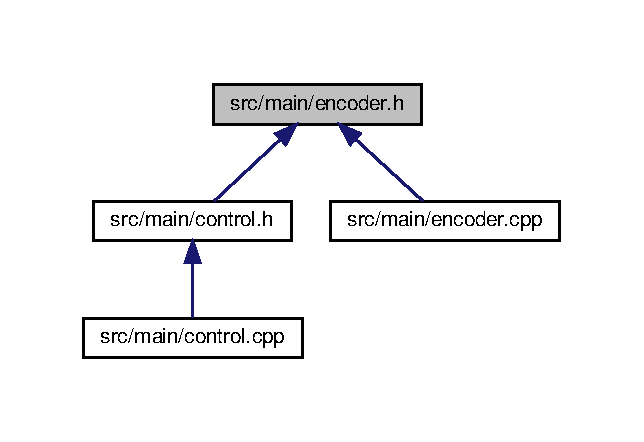
\includegraphics[width=309pt]{encoder_8h__dep__incl}
\end{center}
\end{figure}
\subsection*{Classes}
\begin{DoxyCompactItemize}
\item 
class \hyperlink{class_encoder}{Encoder}
\begin{DoxyCompactList}\small\item\em \hyperlink{class_encoder}{Encoder} class is responsible for reading rotary encoder input. \end{DoxyCompactList}\end{DoxyCompactItemize}


\subsection{Detailed Description}
Declaration of \hyperlink{class_encoder}{Encoder} class. 

\begin{DoxyAuthor}{Author}
Valentin Mercy (\href{https://github.com/vmercy}{\tt https\+://github.\+com/vmercy}) 
\end{DoxyAuthor}
\begin{DoxyVersion}{Version}
0.\+1 
\end{DoxyVersion}
\begin{DoxyDate}{Date}
2020-\/11-\/27
\end{DoxyDate}
\begin{DoxyCopyright}{Copyright}
Copyright (c) 2020 
\end{DoxyCopyright}

\hypertarget{frame_8h}{}\section{src/main/frame.h File Reference}
\label{frame_8h}\index{src/main/frame.\+h@{src/main/frame.\+h}}


Declaration of frame types and incoming\+Frame class.  


{\ttfamily \#include \char`\"{}battery.\+h\char`\"{}}\newline
{\ttfamily \#include $<$Arduino.\+h$>$}\newline
Include dependency graph for frame.\+h\+:\nopagebreak
\begin{figure}[H]
\begin{center}
\leavevmode
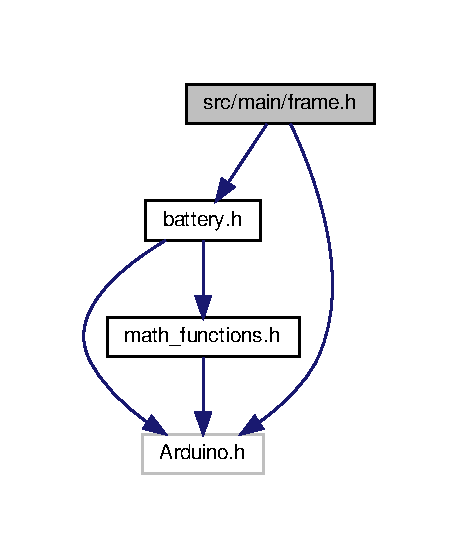
\includegraphics[width=220pt]{frame_8h__incl}
\end{center}
\end{figure}
This graph shows which files directly or indirectly include this file\+:\nopagebreak
\begin{figure}[H]
\begin{center}
\leavevmode
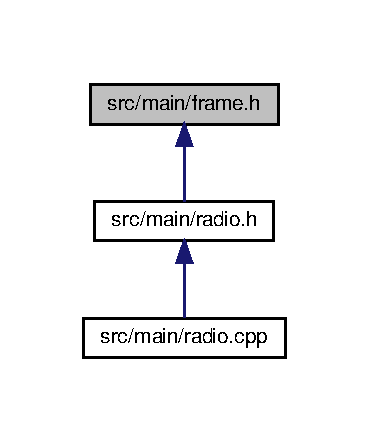
\includegraphics[width=177pt]{frame_8h__dep__incl}
\end{center}
\end{figure}
\subsection*{Classes}
\begin{DoxyCompactItemize}
\item 
struct \hyperlink{struct_tto_p_data_frame}{Tto\+P\+Data\+Frame}
\begin{DoxyCompactList}\small\item\em Struct composed with all data contained in a frame sent from the Transmitter to the Plane. \end{DoxyCompactList}\item 
struct \hyperlink{struct_pto_t_data_frame}{Pto\+T\+Data\+Frame}
\begin{DoxyCompactList}\small\item\em Struct composed with all data contained in a frame sent from the Plane to the Transmitter. \end{DoxyCompactList}\end{DoxyCompactItemize}


\subsection{Detailed Description}
Declaration of frame types and incoming\+Frame class. 

\begin{DoxyAuthor}{Author}
Valentin Mercy (\href{https://github.com/vmercy}{\tt https\+://github.\+com/vmercy}) 
\end{DoxyAuthor}
\begin{DoxyVersion}{Version}
0.\+1 
\end{DoxyVersion}
\begin{DoxyDate}{Date}
2020-\/11-\/24
\end{DoxyDate}
\begin{DoxyCopyright}{Copyright}
Copyright (c) 2020 
\end{DoxyCopyright}

\hypertarget{joystick_8cpp}{}\section{src/main/joystick.cpp File Reference}
\label{joystick_8cpp}\index{src/main/joystick.\+cpp@{src/main/joystick.\+cpp}}


Definition of \hyperlink{class_joystick}{Joystick} class.  


{\ttfamily \#include \char`\"{}joystick.\+h\char`\"{}}\newline
Include dependency graph for joystick.\+cpp\+:
\nopagebreak
\begin{figure}[H]
\begin{center}
\leavevmode
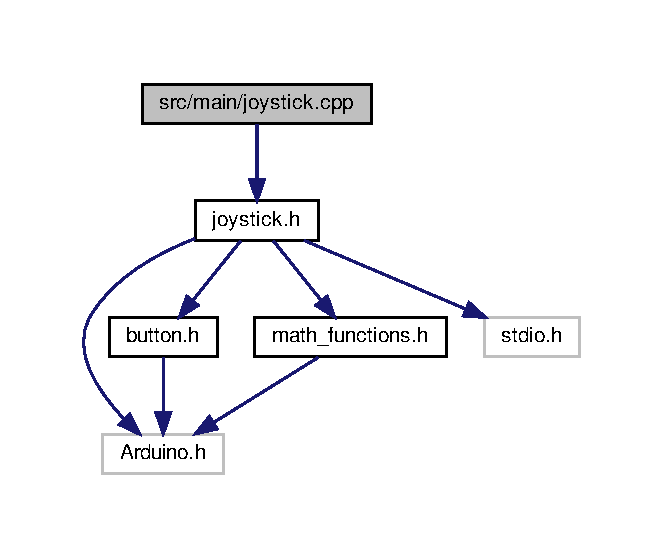
\includegraphics[width=316pt]{joystick_8cpp__incl}
\end{center}
\end{figure}


\subsection{Detailed Description}
Definition of \hyperlink{class_joystick}{Joystick} class. 

\begin{DoxyAuthor}{Author}
Valentin Mercy (\href{https://github.com/vmercy}{\tt https\+://github.\+com/vmercy}) 
\end{DoxyAuthor}
\begin{DoxyVersion}{Version}
0.\+1 
\end{DoxyVersion}
\begin{DoxyDate}{Date}
2020-\/11-\/26
\end{DoxyDate}
\begin{DoxyCopyright}{Copyright}
Copyright (c) 2020 
\end{DoxyCopyright}

\hypertarget{joystick_8h}{}\section{src/main/joystick.h File Reference}
\label{joystick_8h}\index{src/main/joystick.\+h@{src/main/joystick.\+h}}


Declaration of \hyperlink{class_joystick}{Joystick} class.  


{\ttfamily \#include $<$Arduino.\+h$>$}\newline
{\ttfamily \#include \char`\"{}button.\+h\char`\"{}}\newline
{\ttfamily \#include \char`\"{}math\+\_\+functions.\+h\char`\"{}}\newline
{\ttfamily \#include $<$stdio.\+h$>$}\newline
Include dependency graph for joystick.\+h\+:\nopagebreak
\begin{figure}[H]
\begin{center}
\leavevmode
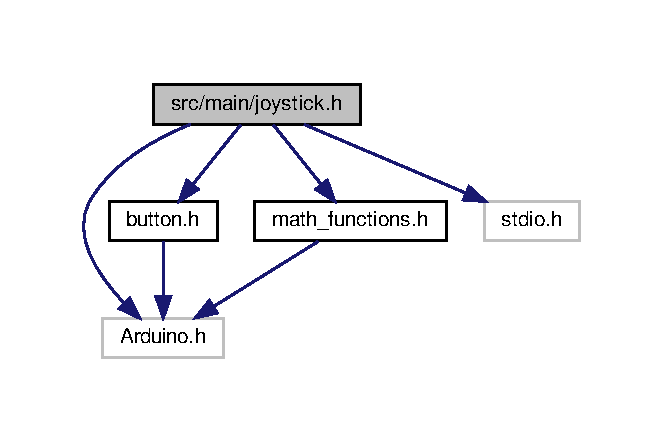
\includegraphics[width=318pt]{joystick_8h__incl}
\end{center}
\end{figure}
This graph shows which files directly or indirectly include this file\+:\nopagebreak
\begin{figure}[H]
\begin{center}
\leavevmode
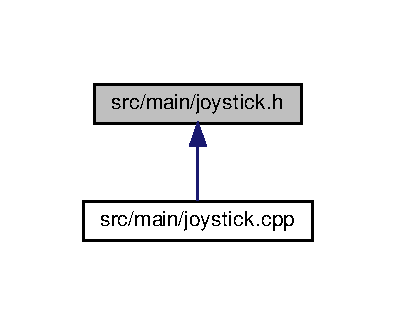
\includegraphics[width=309pt]{joystick_8h__dep__incl}
\end{center}
\end{figure}
\subsection*{Classes}
\begin{DoxyCompactItemize}
\item 
class \hyperlink{class_joystick}{Joystick}
\end{DoxyCompactItemize}
\subsection*{Macros}
\begin{DoxyCompactItemize}
\item 
\mbox{\Hypertarget{joystick_8h_a7a142b105e6b647b7c90d48c75bb3bc5}\label{joystick_8h_a7a142b105e6b647b7c90d48c75bb3bc5}} 
\#define {\bfseries N\+B\+\_\+\+S\+A\+M\+P\+L\+E\+S\+\_\+\+J\+O\+Y\+S\+T\+I\+CK}~10
\item 
\mbox{\Hypertarget{joystick_8h_a35f1467bf87db9e9d057b19e73342bf1}\label{joystick_8h_a35f1467bf87db9e9d057b19e73342bf1}} 
\#define {\bfseries S\+A\+M\+P\+L\+E\+\_\+\+D\+E\+L\+AY}~1
\item 
\mbox{\Hypertarget{joystick_8h_a9eba96a5178f125c87be5a8859a7a630}\label{joystick_8h_a9eba96a5178f125c87be5a8859a7a630}} 
\#define {\bfseries I\+D\+L\+E\+\_\+\+T\+O\+L\+E\+R\+A\+N\+CE}~1
\item 
\mbox{\Hypertarget{joystick_8h_a58d7eeb94e7c66d063a55b586735b887}\label{joystick_8h_a58d7eeb94e7c66d063a55b586735b887}} 
\#define {\bfseries J\+O\+Y\+S\+T\+I\+C\+K\+\_\+\+M\+I\+N\+\_\+\+P\+O\+S\+I\+T\+I\+ON}~0
\item 
\mbox{\Hypertarget{joystick_8h_aaa23ccac0cd817d10bc1dff3e2c90c41}\label{joystick_8h_aaa23ccac0cd817d10bc1dff3e2c90c41}} 
\#define {\bfseries J\+O\+Y\+S\+T\+I\+C\+K\+\_\+\+M\+A\+X\+\_\+\+P\+O\+S\+I\+T\+I\+ON}~255
\item 
\mbox{\Hypertarget{joystick_8h_a4e85f0ba2181c6add5d3c03276b2f3cb}\label{joystick_8h_a4e85f0ba2181c6add5d3c03276b2f3cb}} 
\#define {\bfseries U\+N\+D\+E\+F\+I\+N\+E\+D\+\_\+\+P\+O\+S\+I\+T\+I\+ON}~0
\item 
\mbox{\Hypertarget{joystick_8h_a85d1ada414f4f1f10df50ef254c79c75}\label{joystick_8h_a85d1ada414f4f1f10df50ef254c79c75}} 
\#define {\bfseries B\+O\+T\+T\+O\+M\+\_\+\+L\+E\+FT}~1
\item 
\mbox{\Hypertarget{joystick_8h_a9c05beaff6794473029413f2d78589f1}\label{joystick_8h_a9c05beaff6794473029413f2d78589f1}} 
\#define {\bfseries B\+O\+T\+T\+O\+M\+\_\+\+R\+I\+G\+HT}~2
\item 
\mbox{\Hypertarget{joystick_8h_a1b0c3083ed9973911de4767aa677f673}\label{joystick_8h_a1b0c3083ed9973911de4767aa677f673}} 
\#define {\bfseries T\+O\+P\+\_\+\+L\+E\+FT}~3
\item 
\mbox{\Hypertarget{joystick_8h_a80473d4f5c5ff853d7342618295ba314}\label{joystick_8h_a80473d4f5c5ff853d7342618295ba314}} 
\#define {\bfseries T\+O\+P\+\_\+\+R\+I\+G\+HT}~4
\end{DoxyCompactItemize}


\subsection{Detailed Description}
Declaration of \hyperlink{class_joystick}{Joystick} class. 

\begin{DoxyAuthor}{Author}
Valentin Mercy (\href{https://github.com/vmercy}{\tt https\+://github.\+com/vmercy}) 
\end{DoxyAuthor}
\begin{DoxyVersion}{Version}
0.\+1 
\end{DoxyVersion}
\begin{DoxyDate}{Date}
2020-\/11-\/26
\end{DoxyDate}
\begin{DoxyCopyright}{Copyright}
Copyright (c) 2020 
\end{DoxyCopyright}

\hypertarget{lcd__bitmaps_8h}{}\section{src/main/lcd\+\_\+bitmaps.h File Reference}
\label{lcd__bitmaps_8h}\index{src/main/lcd\+\_\+bitmaps.\+h@{src/main/lcd\+\_\+bitmaps.\+h}}


Contain arrays describing btmaps do display on main L\+CD.  




\subsection{Detailed Description}
Contain arrays describing btmaps do display on main L\+CD. 

\begin{DoxyAuthor}{Author}
Valentin Mercy (\href{https://github.com/vmercy}{\tt https\+://github.\+com/vmercy}) 
\end{DoxyAuthor}
\begin{DoxyVersion}{Version}
0.\+1 
\end{DoxyVersion}
\begin{DoxyDate}{Date}
2020-\/12-\/02
\end{DoxyDate}
\begin{DoxyCopyright}{Copyright}
Copyright (c) 2020 
\end{DoxyCopyright}

\hypertarget{lcdscreen_8cpp}{}\section{src/main/lcdscreen.cpp File Reference}
\label{lcdscreen_8cpp}\index{src/main/lcdscreen.\+cpp@{src/main/lcdscreen.\+cpp}}


Definition of \hyperlink{class_l_c_d_screen}{L\+C\+D\+Screen} class.  


{\ttfamily \#include \char`\"{}lcdscreen.\+h\char`\"{}}\newline
Include dependency graph for lcdscreen.\+cpp\+:\nopagebreak
\begin{figure}[H]
\begin{center}
\leavevmode
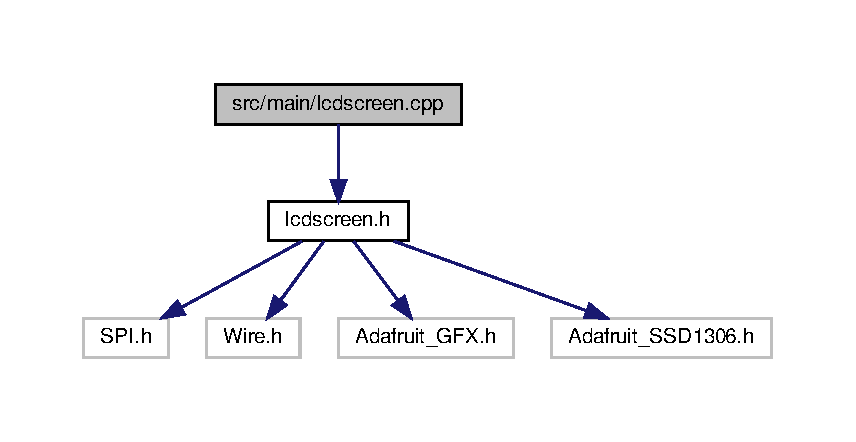
\includegraphics[width=350pt]{lcdscreen_8cpp__incl}
\end{center}
\end{figure}


\subsection{Detailed Description}
Definition of \hyperlink{class_l_c_d_screen}{L\+C\+D\+Screen} class. 

\begin{DoxyAuthor}{Author}
Valentin Mercy (\href{https://github.com/vmercy}{\tt https\+://github.\+com/vmercy}) 
\end{DoxyAuthor}
\begin{DoxyVersion}{Version}
0.\+1 
\end{DoxyVersion}
\begin{DoxyDate}{Date}
2020-\/11-\/28
\end{DoxyDate}
\begin{DoxyCopyright}{Copyright}
Copyright (c) 2020 
\end{DoxyCopyright}

\hypertarget{lcdscreen_8h}{}\section{src/main/lcdscreen.h File Reference}
\label{lcdscreen_8h}\index{src/main/lcdscreen.\+h@{src/main/lcdscreen.\+h}}


Declaration of \hyperlink{class_l_c_d_screen}{L\+C\+D\+Screen} class.  


{\ttfamily \#include $<$S\+P\+I.\+h$>$}\newline
{\ttfamily \#include $<$Wire.\+h$>$}\newline
{\ttfamily \#include $<$Adafruit\+\_\+\+G\+F\+X.\+h$>$}\newline
{\ttfamily \#include $<$Adafruit\+\_\+\+S\+S\+D1306.\+h$>$}\newline
Include dependency graph for lcdscreen.\+h\+:\nopagebreak
\begin{figure}[H]
\begin{center}
\leavevmode
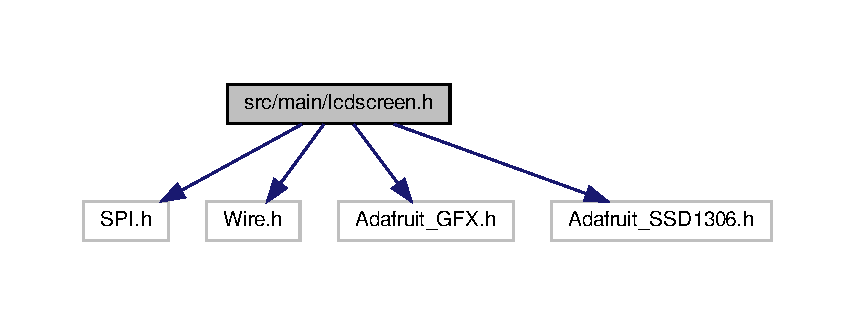
\includegraphics[width=350pt]{lcdscreen_8h__incl}
\end{center}
\end{figure}
This graph shows which files directly or indirectly include this file\+:\nopagebreak
\begin{figure}[H]
\begin{center}
\leavevmode
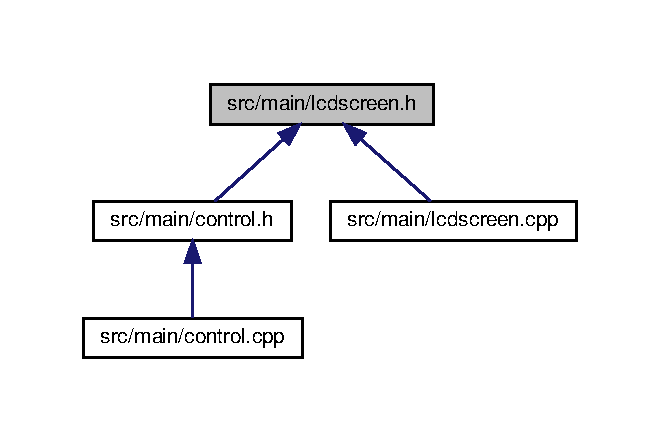
\includegraphics[width=317pt]{lcdscreen_8h__dep__incl}
\end{center}
\end{figure}
\subsection*{Classes}
\begin{DoxyCompactItemize}
\item 
class \hyperlink{class_l_c_d_screen}{L\+C\+D\+Screen}
\begin{DoxyCompactList}\small\item\em \hyperlink{class_l_c_d_screen}{L\+C\+D\+Screen} class is responsible for displaying informations on an S\+S\+D1306 I2C screen. \end{DoxyCompactList}\end{DoxyCompactItemize}
\subsection*{Macros}
\begin{DoxyCompactItemize}
\item 
\mbox{\Hypertarget{lcdscreen_8h_a2cd109632a6dcccaa80b43561b1ab700}\label{lcdscreen_8h_a2cd109632a6dcccaa80b43561b1ab700}} 
\#define {\bfseries S\+C\+R\+E\+E\+N\+\_\+\+W\+I\+D\+TH}~128
\item 
\mbox{\Hypertarget{lcdscreen_8h_a6974d08a74da681b3957b2fead2608b8}\label{lcdscreen_8h_a6974d08a74da681b3957b2fead2608b8}} 
\#define {\bfseries S\+C\+R\+E\+E\+N\+\_\+\+H\+E\+I\+G\+HT}~32
\item 
\mbox{\Hypertarget{lcdscreen_8h_a619e07239fb3b9b14d40646ab41d5b4f}\label{lcdscreen_8h_a619e07239fb3b9b14d40646ab41d5b4f}} 
\#define {\bfseries O\+L\+E\+D\+\_\+\+R\+E\+S\+ET}~4
\item 
\mbox{\Hypertarget{lcdscreen_8h_a88b90a6366ac67c662321171f5b1fe34}\label{lcdscreen_8h_a88b90a6366ac67c662321171f5b1fe34}} 
\#define {\bfseries L\+O\+G\+O\+\_\+\+H\+E\+I\+G\+HT}~64
\item 
\mbox{\Hypertarget{lcdscreen_8h_aaca826667b185ef968585f830dcec417}\label{lcdscreen_8h_aaca826667b185ef968585f830dcec417}} 
\#define {\bfseries L\+O\+G\+O\+\_\+\+W\+I\+D\+TH}~128
\end{DoxyCompactItemize}


\subsection{Detailed Description}
Declaration of \hyperlink{class_l_c_d_screen}{L\+C\+D\+Screen} class. 

\begin{DoxyAuthor}{Author}
Valentin Mercy (\href{https://github.com/vmercy}{\tt https\+://github.\+com/vmercy}) 
\end{DoxyAuthor}
\begin{DoxyVersion}{Version}
0.\+1 
\end{DoxyVersion}
\begin{DoxyDate}{Date}
2020-\/11-\/28
\end{DoxyDate}
\begin{DoxyCopyright}{Copyright}
Copyright (c) 2020 
\end{DoxyCopyright}

\hypertarget{led_8cpp}{}\section{src/main/led.cpp File Reference}
\label{led_8cpp}\index{src/main/led.\+cpp@{src/main/led.\+cpp}}


Definition of \hyperlink{class_led}{Led} class.  


{\ttfamily \#include \char`\"{}led.\+h\char`\"{}}\newline
Include dependency graph for led.\+cpp\+:
\nopagebreak
\begin{figure}[H]
\begin{center}
\leavevmode
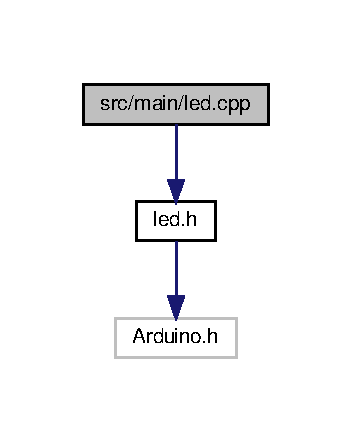
\includegraphics[width=169pt]{led_8cpp__incl}
\end{center}
\end{figure}


\subsection{Detailed Description}
Definition of \hyperlink{class_led}{Led} class. 

\begin{DoxyAuthor}{Author}
Valentin Mercy (\href{https://github.com/vmercy}{\tt https\+://github.\+com/vmercy}) 
\end{DoxyAuthor}
\begin{DoxyVersion}{Version}
0.\+1 
\end{DoxyVersion}
\begin{DoxyDate}{Date}
2020-\/11-\/26
\end{DoxyDate}
\begin{DoxyCopyright}{Copyright}
Copyright (c) 2020 
\end{DoxyCopyright}

\hypertarget{led_8h}{}\section{src/main/led.h File Reference}
\label{led_8h}\index{src/main/led.\+h@{src/main/led.\+h}}


Declaration of \hyperlink{class_led}{Led} class.  


{\ttfamily \#include $<$Arduino.\+h$>$}\newline
Include dependency graph for led.\+h\+:\nopagebreak
\begin{figure}[H]
\begin{center}
\leavevmode
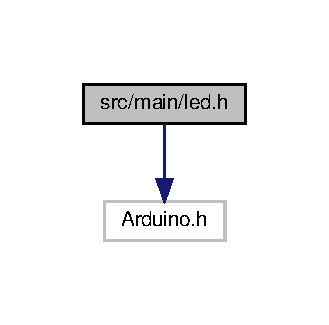
\includegraphics[width=158pt]{led_8h__incl}
\end{center}
\end{figure}
This graph shows which files directly or indirectly include this file\+:\nopagebreak
\begin{figure}[H]
\begin{center}
\leavevmode
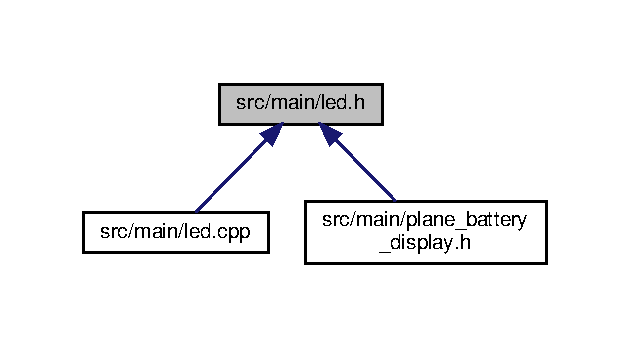
\includegraphics[width=303pt]{led_8h__dep__incl}
\end{center}
\end{figure}
\subsection*{Classes}
\begin{DoxyCompactItemize}
\item 
class \hyperlink{class_led}{Led}
\end{DoxyCompactItemize}
\subsection*{Macros}
\begin{DoxyCompactItemize}
\item 
\mbox{\Hypertarget{led_8h_a2476623e11f86f8423fd34d4a09e4f4a}\label{led_8h_a2476623e11f86f8423fd34d4a09e4f4a}} 
\#define {\bfseries L\+E\+D\+\_\+\+S\+T\+A\+T\+ES}
\item 
\mbox{\Hypertarget{led_8h_ad76d1750a6cdeebd506bfcd6752554d2}\label{led_8h_ad76d1750a6cdeebd506bfcd6752554d2}} 
\#define {\bfseries ON}~1
\item 
\mbox{\Hypertarget{led_8h_a29e413f6725b2ba32d165ffaa35b01e5}\label{led_8h_a29e413f6725b2ba32d165ffaa35b01e5}} 
\#define {\bfseries O\+FF}~0
\end{DoxyCompactItemize}


\subsection{Detailed Description}
Declaration of \hyperlink{class_led}{Led} class. 

\begin{DoxyAuthor}{Author}
Valentin Mercy (\href{https://github.com/vmercy}{\tt https\+://github.\+com/vmercy}) 
\end{DoxyAuthor}
\begin{DoxyVersion}{Version}
0.\+1 
\end{DoxyVersion}
\begin{DoxyDate}{Date}
2020-\/11-\/26
\end{DoxyDate}
\begin{DoxyCopyright}{Copyright}
Copyright (c) 2020 
\end{DoxyCopyright}

\hypertarget{math__functions_8h}{}\section{src/main/math\+\_\+functions.h File Reference}
\label{math__functions_8h}\index{src/main/math\+\_\+functions.\+h@{src/main/math\+\_\+functions.\+h}}


Declaration of a set of mathematical functions.  


{\ttfamily \#include $<$Arduino.\+h$>$}\newline
Include dependency graph for math\+\_\+functions.\+h\+:
\nopagebreak
\begin{figure}[H]
\begin{center}
\leavevmode
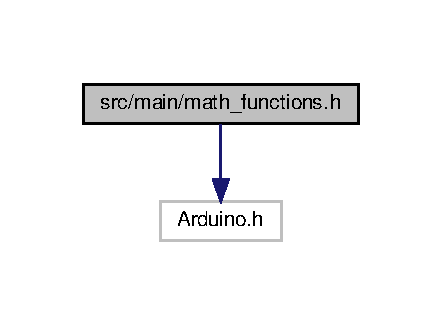
\includegraphics[width=212pt]{math__functions_8h__incl}
\end{center}
\end{figure}
This graph shows which files directly or indirectly include this file\+:
\nopagebreak
\begin{figure}[H]
\begin{center}
\leavevmode
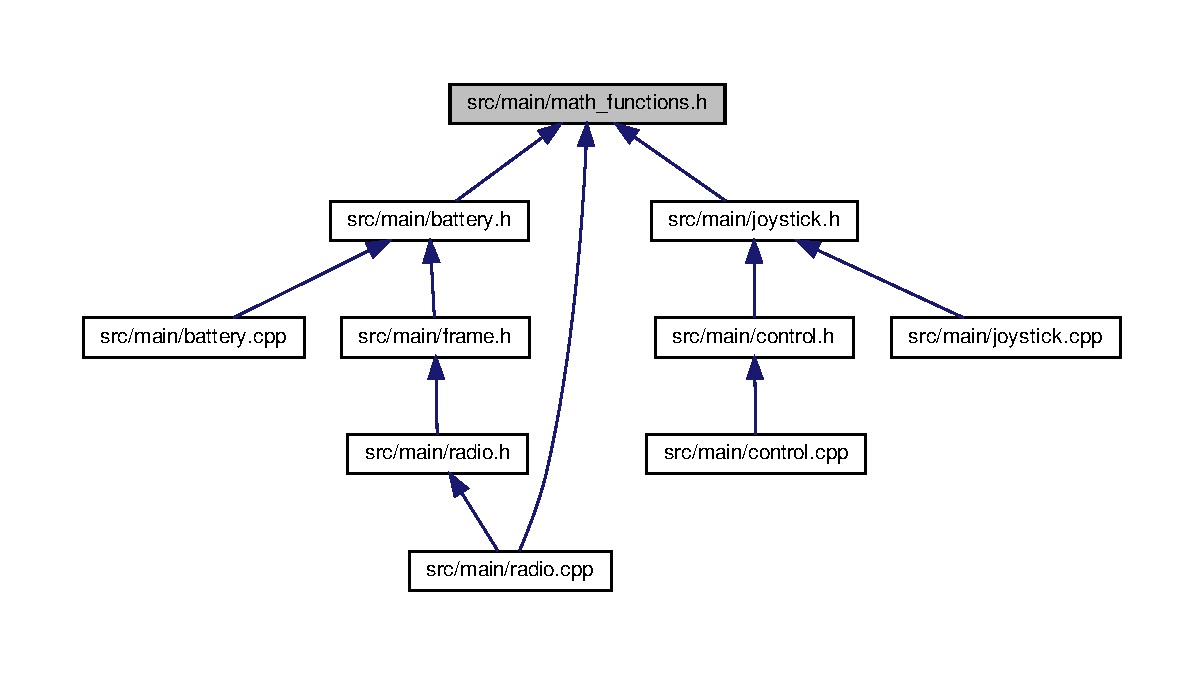
\includegraphics[width=350pt]{math__functions_8h__dep__incl}
\end{center}
\end{figure}
\subsection*{Namespaces}
\begin{DoxyCompactItemize}
\item 
 \hyperlink{namespacemath_functions}{math\+Functions}
\begin{DoxyCompactList}\small\item\em collection of useful templated math functions \end{DoxyCompactList}\end{DoxyCompactItemize}
\subsection*{Functions}
\begin{DoxyCompactItemize}
\item 
{\footnotesize template$<$typename T , typename K $>$ }\\T \hyperlink{namespacemath_functions_addb45716cc0631d67e6cb6a913336491}{math\+Functions\+::sum} (K data\+Array\+\_\+p\mbox{[}$\,$\mbox{]}, uint8\+\_\+t size\+\_\+p)
\begin{DoxyCompactList}\small\item\em computes a sum \end{DoxyCompactList}\item 
{\footnotesize template$<$typename T , typename K , typename U  = K$>$ }\\T \hyperlink{namespacemath_functions_a5b9bc0e0bf8f4e65a9177b8274c594ef}{math\+Functions\+::mean} (K data\+Array\+\_\+p\mbox{[}$\,$\mbox{]}, uint8\+\_\+t size\+\_\+p)
\begin{DoxyCompactList}\small\item\em computes a mean value \end{DoxyCompactList}\item 
{\footnotesize template$<$typename T , typename K  = T$>$ }\\K \hyperlink{namespacemath_functions_a32a0226ce7d0593d33c203874e28397e}{math\+Functions\+::extract\+Digit} (T number\+\_\+p, uint8\+\_\+t digit\+Select\+\_\+p=0, uint8\+\_\+t base\+\_\+p=10)
\begin{DoxyCompactList}\small\item\em extracts digit from a number \end{DoxyCompactList}\item 
{\footnotesize template$<$typename T , typename U  = T, typename K  = U$>$ }\\K \hyperlink{namespacemath_functions_a65a3e03a8f5216b86440247de2023aae}{math\+Functions\+::map} (T base, T min\+Base, T max\+Base, U new\+Min, U new\+Max)
\begin{DoxyCompactList}\small\item\em Re-\/maps a number from one range to another. \end{DoxyCompactList}\end{DoxyCompactItemize}


\subsection{Detailed Description}
Declaration of a set of mathematical functions. 

\begin{DoxyAuthor}{Author}
Valentin Mercy (\href{https://github.com/vmercy}{\tt https\+://github.\+com/vmercy}) 
\end{DoxyAuthor}
\begin{DoxyVersion}{Version}
0.\+1 
\end{DoxyVersion}
\begin{DoxyDate}{Date}
2020-\/11-\/26
\end{DoxyDate}
\begin{DoxyCopyright}{Copyright}
Copyright (c) 2020 
\end{DoxyCopyright}

\hypertarget{radio_8cpp}{}\section{src/main/radio.cpp File Reference}
\label{radio_8cpp}\index{src/main/radio.\+cpp@{src/main/radio.\+cpp}}


Definition of radio class.  


{\ttfamily \#include $<$Arduino.\+h$>$}\newline
{\ttfamily \#include \char`\"{}radio.\+h\char`\"{}}\newline
{\ttfamily \#include \char`\"{}math\+\_\+functions.\+h\char`\"{}}\newline
Include dependency graph for radio.\+cpp\+:
\nopagebreak
\begin{figure}[H]
\begin{center}
\leavevmode
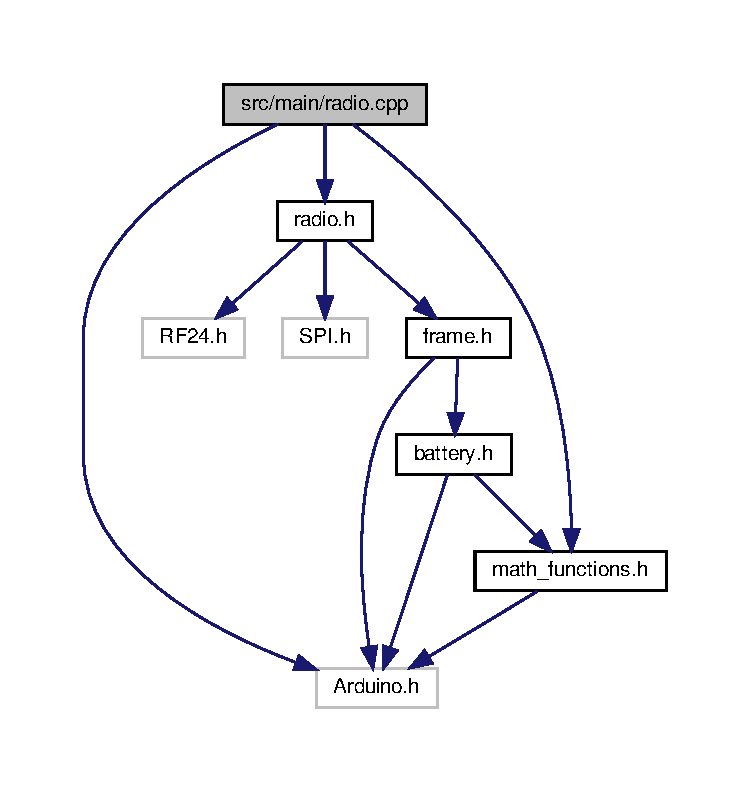
\includegraphics[width=350pt]{radio_8cpp__incl}
\end{center}
\end{figure}


\subsection{Detailed Description}
Definition of radio class. 

\begin{DoxyAuthor}{Author}
Valentin Mercy (\href{https://github.com/vmercy}{\tt https\+://github.\+com/vmercy}) 
\end{DoxyAuthor}
\begin{DoxyVersion}{Version}
0.\+1 
\end{DoxyVersion}
\begin{DoxyDate}{Date}
2020-\/11-\/24
\end{DoxyDate}
\begin{DoxyCopyright}{Copyright}
Copyright (c) 2020 
\end{DoxyCopyright}

\hypertarget{radio_8h}{}\section{src/main/radio.h File Reference}
\label{radio_8h}\index{src/main/radio.\+h@{src/main/radio.\+h}}


Declaration of radio class.  


{\ttfamily \#include $<$R\+F24.\+h$>$}\newline
{\ttfamily \#include $<$S\+P\+I.\+h$>$}\newline
{\ttfamily \#include \char`\"{}frame.\+h\char`\"{}}\newline
Include dependency graph for radio.\+h\+:
\nopagebreak
\begin{figure}[H]
\begin{center}
\leavevmode
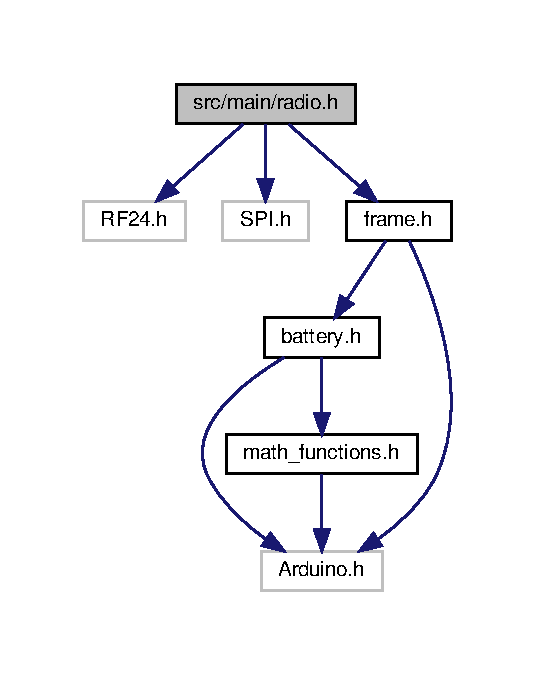
\includegraphics[width=257pt]{radio_8h__incl}
\end{center}
\end{figure}
This graph shows which files directly or indirectly include this file\+:
\nopagebreak
\begin{figure}[H]
\begin{center}
\leavevmode
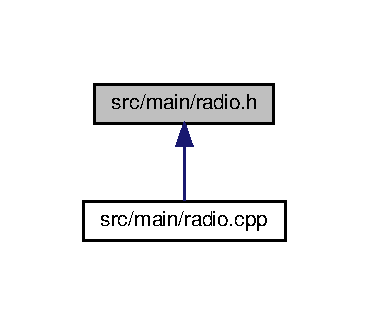
\includegraphics[width=177pt]{radio_8h__dep__incl}
\end{center}
\end{figure}
\subsection*{Classes}
\begin{DoxyCompactItemize}
\item 
class \hyperlink{class_radio}{Radio}
\begin{DoxyCompactList}\small\item\em \hyperlink{class_radio}{Radio} class responsible for communicating with the \hyperlink{class_radio}{Radio} Transmitter on the ground. \end{DoxyCompactList}\end{DoxyCompactItemize}
\subsection*{Macros}
\begin{DoxyCompactItemize}
\item 
\mbox{\Hypertarget{radio_8h_ab3e8a5a8c7f4714d547d49fa36153f45}\label{radio_8h_ab3e8a5a8c7f4714d547d49fa36153f45}} 
\#define {\bfseries A\+U\+T\+H\+E\+N\+T\+I\+C\+A\+T\+I\+O\+N\+\_\+\+P\+IN}~1234
\end{DoxyCompactItemize}


\subsection{Detailed Description}
Declaration of radio class. 

\begin{DoxyAuthor}{Author}
Valentin Mercy (\href{https://github.com/vmercy}{\tt https\+://github.\+com/vmercy}) 
\end{DoxyAuthor}
\begin{DoxyVersion}{Version}
0.\+1 
\end{DoxyVersion}
\begin{DoxyDate}{Date}
2020-\/11-\/24
\end{DoxyDate}
\begin{DoxyCopyright}{Copyright}
Copyright (c) 2020 
\end{DoxyCopyright}

\hypertarget{rgbled_8cpp}{}\section{src/main/rgbled.cpp File Reference}
\label{rgbled_8cpp}\index{src/main/rgbled.\+cpp@{src/main/rgbled.\+cpp}}


Definition of \hyperlink{class_r_g_b_led}{R\+G\+B\+Led} class.  


{\ttfamily \#include \char`\"{}rgbled.\+h\char`\"{}}\newline
Include dependency graph for rgbled.\+cpp\+:\nopagebreak
\begin{figure}[H]
\begin{center}
\leavevmode
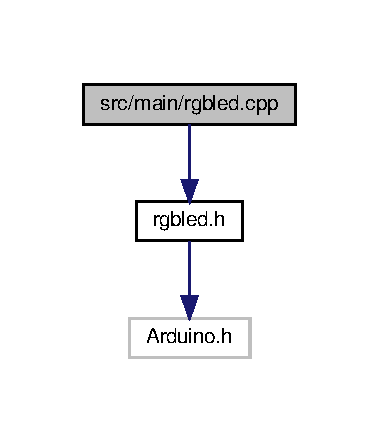
\includegraphics[width=182pt]{rgbled_8cpp__incl}
\end{center}
\end{figure}


\subsection{Detailed Description}
Definition of \hyperlink{class_r_g_b_led}{R\+G\+B\+Led} class. 

\begin{DoxyAuthor}{Author}
Valentin Mercy (\href{https://github.com/vmercy}{\tt https\+://github.\+com/vmercy}) 
\end{DoxyAuthor}
\begin{DoxyVersion}{Version}
0.\+1 
\end{DoxyVersion}
\begin{DoxyDate}{Date}
2020-\/11-\/25
\end{DoxyDate}
\begin{DoxyCopyright}{Copyright}
Copyright (c) 2020 
\end{DoxyCopyright}

\hypertarget{rgbled_8h}{}\section{src/main/rgbled.h File Reference}
\label{rgbled_8h}\index{src/main/rgbled.\+h@{src/main/rgbled.\+h}}


Declaration of \hyperlink{class_r_g_b_led}{R\+G\+B\+Led} class.  


{\ttfamily \#include $<$Arduino.\+h$>$}\newline
Include dependency graph for rgbled.\+h\+:
\nopagebreak
\begin{figure}[H]
\begin{center}
\leavevmode
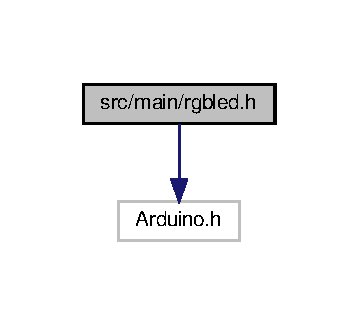
\includegraphics[width=172pt]{rgbled_8h__incl}
\end{center}
\end{figure}
This graph shows which files directly or indirectly include this file\+:
\nopagebreak
\begin{figure}[H]
\begin{center}
\leavevmode
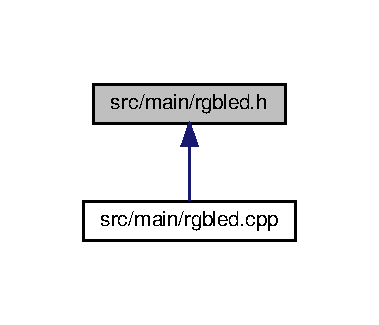
\includegraphics[width=182pt]{rgbled_8h__dep__incl}
\end{center}
\end{figure}
\subsection*{Classes}
\begin{DoxyCompactItemize}
\item 
class \hyperlink{class_r_g_b_led}{R\+G\+B\+Led}
\begin{DoxyCompactList}\small\item\em \hyperlink{class_r_g_b_led}{R\+G\+B\+Led} class is responsible for displaying colors on an R\+GB \hyperlink{class_led}{Led}. \end{DoxyCompactList}\end{DoxyCompactItemize}
\subsection*{Macros}
\begin{DoxyCompactItemize}
\item 
\mbox{\Hypertarget{rgbled_8h_ac8014b990c5aab17a8f75a7d63fc56d6}\label{rgbled_8h_ac8014b990c5aab17a8f75a7d63fc56d6}} 
\#define {\bfseries R\+G\+B\+\_\+\+C\+O\+M\+M\+O\+N\+\_\+\+C\+A\+T\+H\+O\+DE}~0
\item 
\mbox{\Hypertarget{rgbled_8h_a7d37455f2706249fcd3a5f41772c87ba}\label{rgbled_8h_a7d37455f2706249fcd3a5f41772c87ba}} 
\#define {\bfseries R\+G\+B\+\_\+\+C\+O\+M\+M\+O\+N\+\_\+\+A\+N\+O\+DE}~1
\item 
\mbox{\Hypertarget{rgbled_8h_a8d23feea868a983c8c2b661e1e16972f}\label{rgbled_8h_a8d23feea868a983c8c2b661e1e16972f}} 
\#define {\bfseries R\+ED}~0
\item 
\mbox{\Hypertarget{rgbled_8h_acfbc006ea433ad708fdee3e82996e721}\label{rgbled_8h_acfbc006ea433ad708fdee3e82996e721}} 
\#define {\bfseries G\+R\+E\+EN}~1
\item 
\mbox{\Hypertarget{rgbled_8h_a79d10e672abb49ad63eeaa8aaef57c38}\label{rgbled_8h_a79d10e672abb49ad63eeaa8aaef57c38}} 
\#define {\bfseries B\+L\+UE}~2
\item 
\mbox{\Hypertarget{rgbled_8h_ad243f93c16bc4c1d3e0a13b84421d760}\label{rgbled_8h_ad243f93c16bc4c1d3e0a13b84421d760}} 
\#define {\bfseries C\+Y\+AN}~3
\item 
\mbox{\Hypertarget{rgbled_8h_a6f699060902f800f12aaae150f3a708e}\label{rgbled_8h_a6f699060902f800f12aaae150f3a708e}} 
\#define {\bfseries M\+A\+G\+E\+N\+TA}~4
\item 
\mbox{\Hypertarget{rgbled_8h_abf681265909adf3d3e8116c93c0ba179}\label{rgbled_8h_abf681265909adf3d3e8116c93c0ba179}} 
\#define {\bfseries Y\+E\+L\+L\+OW}~5
\item 
\mbox{\Hypertarget{rgbled_8h_a87b537f5fa5c109d3c05c13d6b18f382}\label{rgbled_8h_a87b537f5fa5c109d3c05c13d6b18f382}} 
\#define {\bfseries W\+H\+I\+TE}~6
\item 
\mbox{\Hypertarget{rgbled_8h_a2476623e11f86f8423fd34d4a09e4f4a}\label{rgbled_8h_a2476623e11f86f8423fd34d4a09e4f4a}} 
\#define {\bfseries L\+E\+D\+\_\+\+S\+T\+A\+T\+ES}
\item 
\mbox{\Hypertarget{rgbled_8h_ad76d1750a6cdeebd506bfcd6752554d2}\label{rgbled_8h_ad76d1750a6cdeebd506bfcd6752554d2}} 
\#define {\bfseries ON}~1
\item 
\mbox{\Hypertarget{rgbled_8h_a29e413f6725b2ba32d165ffaa35b01e5}\label{rgbled_8h_a29e413f6725b2ba32d165ffaa35b01e5}} 
\#define {\bfseries O\+FF}~0
\end{DoxyCompactItemize}


\subsection{Detailed Description}
Declaration of \hyperlink{class_r_g_b_led}{R\+G\+B\+Led} class. 

\begin{DoxyAuthor}{Author}
Valentin Mercy (\href{https://github.com/vmercy}{\tt https\+://github.\+com/vmercy}) 
\end{DoxyAuthor}
\begin{DoxyVersion}{Version}
0.\+1 
\end{DoxyVersion}
\begin{DoxyDate}{Date}
2020-\/11-\/25
\end{DoxyDate}
\begin{DoxyCopyright}{Copyright}
Copyright (c) 2020 
\end{DoxyCopyright}

\hypertarget{settings_8cpp}{}\section{src/main/settings.cpp File Reference}
\label{settings_8cpp}\index{src/main/settings.\+cpp@{src/main/settings.\+cpp}}


Definition of settings class.  


{\ttfamily \#include \char`\"{}settings.\+h\char`\"{}}\newline
Include dependency graph for settings.\+cpp\+:\nopagebreak
\begin{figure}[H]
\begin{center}
\leavevmode
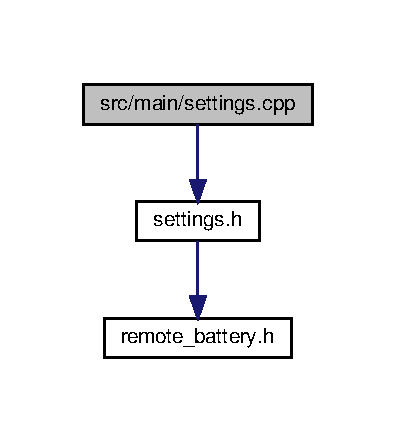
\includegraphics[width=230pt]{settings_8cpp__incl}
\end{center}
\end{figure}


\subsection{Detailed Description}
Definition of settings class. 

\begin{DoxyAuthor}{Author}
Valentin Mercy (\href{https://github.com/vmercy}{\tt https\+://github.\+com/vmercy}) 
\end{DoxyAuthor}
\begin{DoxyVersion}{Version}
0.\+1 
\end{DoxyVersion}
\begin{DoxyDate}{Date}
2020-\/12-\/22
\end{DoxyDate}
\begin{DoxyCopyright}{Copyright}
Copyright (c) 2020 
\end{DoxyCopyright}

\hypertarget{settings_8h}{}\section{src/main/settings.h File Reference}
\label{settings_8h}\index{src/main/settings.\+h@{src/main/settings.\+h}}


Default settings and declaration of settings class.  


{\ttfamily \#include \char`\"{}remote\+\_\+battery.\+h\char`\"{}}\newline
Include dependency graph for settings.\+h\+:\nopagebreak
\begin{figure}[H]
\begin{center}
\leavevmode
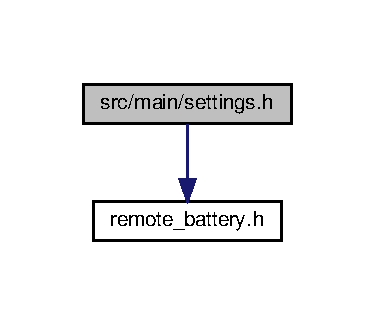
\includegraphics[width=180pt]{settings_8h__incl}
\end{center}
\end{figure}
This graph shows which files directly or indirectly include this file\+:\nopagebreak
\begin{figure}[H]
\begin{center}
\leavevmode
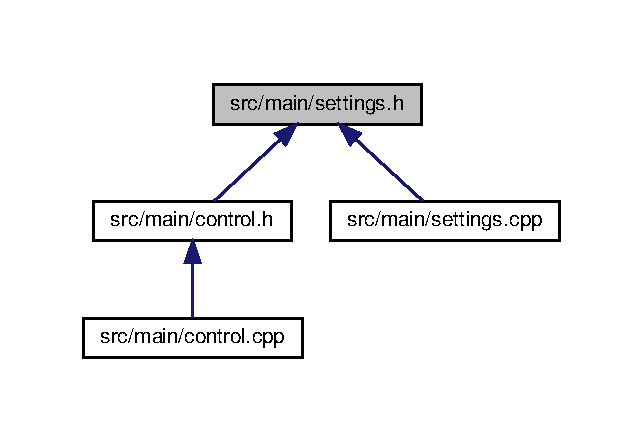
\includegraphics[width=309pt]{settings_8h__dep__incl}
\end{center}
\end{figure}
\subsection*{Classes}
\begin{DoxyCompactItemize}
\item 
class \hyperlink{class_settings}{Settings}
\begin{DoxyCompactList}\small\item\em \hyperlink{class_settings}{Settings} class is responsible for. \end{DoxyCompactList}\end{DoxyCompactItemize}
\subsection*{Macros}
\begin{DoxyCompactItemize}
\item 
\mbox{\Hypertarget{settings_8h_a729564c1f4213a93735615c3f564867e}\label{settings_8h_a729564c1f4213a93735615c3f564867e}} 
\#define {\bfseries N\+B\+\_\+\+B\+O\+O\+L\+\_\+\+S\+E\+T\+T\+I\+N\+GS}~6
\item 
\mbox{\Hypertarget{settings_8h_a72f18aecb7a59e9d9dd9c8f1bf36166c}\label{settings_8h_a72f18aecb7a59e9d9dd9c8f1bf36166c}} 
\#define {\bfseries N\+B\+\_\+\+B\+Y\+T\+E\+\_\+\+S\+E\+T\+T\+I\+N\+GS}~4
\item 
\mbox{\Hypertarget{settings_8h_a44aa650e1c7c5f3cfddc1c41db4fb76f}\label{settings_8h_a44aa650e1c7c5f3cfddc1c41db4fb76f}} 
\#define {\bfseries N\+B\+\_\+\+I\+N\+T\+\_\+\+S\+E\+T\+T\+I\+N\+GS}~0
\item 
\mbox{\Hypertarget{settings_8h_a9083262f2271bd792bea0339109ef108}\label{settings_8h_a9083262f2271bd792bea0339109ef108}} 
\#define {\bfseries N\+B\+\_\+\+S\+E\+T\+T\+I\+N\+GS}~(N\+B\+\_\+\+B\+O\+O\+L\+\_\+\+S\+E\+T\+T\+I\+N\+GS + N\+B\+\_\+\+B\+Y\+T\+E\+\_\+\+S\+E\+T\+T\+I\+N\+GS + N\+B\+\_\+\+I\+N\+T\+\_\+\+S\+E\+T\+T\+I\+N\+GS)
\item 
\mbox{\Hypertarget{settings_8h_a9c78a944348c8f780a556de903ace7bb}\label{settings_8h_a9c78a944348c8f780a556de903ace7bb}} 
\#define {\bfseries R\+E\+V\+E\+R\+T\+\_\+\+P\+O\+W\+ER}~0
\item 
\mbox{\Hypertarget{settings_8h_af2a862d9159f3fb4453be990d268aa13}\label{settings_8h_af2a862d9159f3fb4453be990d268aa13}} 
\#define {\bfseries R\+E\+V\+E\+R\+T\+\_\+\+R\+O\+LL}~1
\item 
\mbox{\Hypertarget{settings_8h_afa1eb82dd2ea8aa729c570ad27bc5308}\label{settings_8h_afa1eb82dd2ea8aa729c570ad27bc5308}} 
\#define {\bfseries R\+E\+V\+E\+R\+T\+\_\+\+Y\+AW}~2
\item 
\mbox{\Hypertarget{settings_8h_a5649594be537decf5e6955014322228c}\label{settings_8h_a5649594be537decf5e6955014322228c}} 
\#define {\bfseries R\+E\+V\+E\+R\+T\+\_\+\+P\+I\+T\+CH}~3
\item 
\mbox{\Hypertarget{settings_8h_aab63f2bf071517f506fb01da19a09f06}\label{settings_8h_aab63f2bf071517f506fb01da19a09f06}} 
\#define {\bfseries E\+N\+A\+B\+L\+E\+\_\+\+B\+U\+Z\+Z\+ER}~4
\item 
\mbox{\Hypertarget{settings_8h_afab00af451ea0747b27f466c04d355b1}\label{settings_8h_afab00af451ea0747b27f466c04d355b1}} 
\#define {\bfseries R\+E\+D\+U\+C\+E\+\_\+\+G\+R\+O\+U\+N\+D\+\_\+\+S\+P\+E\+ED}~5
\item 
\mbox{\Hypertarget{settings_8h_a669c3265d9fecc4f462f71f644225de8}\label{settings_8h_a669c3265d9fecc4f462f71f644225de8}} 
\#define {\bfseries M\+A\+X\+\_\+\+G\+R\+O\+U\+N\+D\+\_\+\+P\+O\+W\+ER}~6
\item 
\mbox{\Hypertarget{settings_8h_a65d999b485fd49b24b03c98367813603}\label{settings_8h_a65d999b485fd49b24b03c98367813603}} 
\#define {\bfseries B\+A\+T\+T\+E\+R\+Y\+\_\+\+C\+E\+L\+L\+\_\+\+A\+L\+E\+R\+T\+\_\+\+V\+O\+L\+T\+A\+GE}~7
\item 
\mbox{\Hypertarget{settings_8h_a3d0dbddf2f4fe415ee4c5bf20d12dc37}\label{settings_8h_a3d0dbddf2f4fe415ee4c5bf20d12dc37}} 
\#define {\bfseries B\+A\+T\+T\+E\+R\+Y\+\_\+\+C\+E\+L\+L\+\_\+\+C\+R\+I\+T\+I\+C\+A\+L\+\_\+\+V\+O\+L\+T\+A\+GE}~8
\item 
\mbox{\Hypertarget{settings_8h_a30cf83698620f60aa7616f0eee28d65e}\label{settings_8h_a30cf83698620f60aa7616f0eee28d65e}} 
\#define {\bfseries A\+U\+T\+O\+T\+H\+R\+U\+S\+T\+\_\+\+C\+U\+R\+S\+O\+R\+\_\+\+S\+T\+EP}~9
\item 
\mbox{\Hypertarget{settings_8h_a4d1284eb184c7665bac3038c3deeb9df}\label{settings_8h_a4d1284eb184c7665bac3038c3deeb9df}} 
\#define {\bfseries D\+E\+F\+A\+U\+L\+T\+\_\+\+R\+E\+V\+E\+R\+T\+\_\+\+P\+O\+W\+ER}~false
\item 
\mbox{\Hypertarget{settings_8h_abdc3ff8e3a386a21cf6f6c0b0d62c6da}\label{settings_8h_abdc3ff8e3a386a21cf6f6c0b0d62c6da}} 
\#define {\bfseries D\+E\+F\+A\+U\+L\+T\+\_\+\+R\+E\+V\+E\+R\+T\+\_\+\+R\+O\+LL}~false
\item 
\mbox{\Hypertarget{settings_8h_aad74eafe605388ae389edcfaed7d2195}\label{settings_8h_aad74eafe605388ae389edcfaed7d2195}} 
\#define {\bfseries D\+E\+F\+A\+U\+L\+T\+\_\+\+R\+E\+V\+E\+R\+T\+\_\+\+Y\+AW}~true
\item 
\mbox{\Hypertarget{settings_8h_aa5c60c1d3d8e81ad1fb4b0b0c8ff2d87}\label{settings_8h_aa5c60c1d3d8e81ad1fb4b0b0c8ff2d87}} 
\#define {\bfseries D\+E\+F\+A\+U\+L\+T\+\_\+\+R\+E\+V\+E\+R\+T\+\_\+\+P\+I\+T\+CH}~false
\item 
\mbox{\Hypertarget{settings_8h_ac7a28224a20859ce1ff0fbf1d292081a}\label{settings_8h_ac7a28224a20859ce1ff0fbf1d292081a}} 
\#define {\bfseries D\+E\+F\+A\+U\+L\+T\+\_\+\+E\+N\+A\+B\+L\+E\+\_\+\+B\+U\+Z\+Z\+ER}~true
\item 
\mbox{\Hypertarget{settings_8h_a706d80f8d27976bab5f28ead571752c9}\label{settings_8h_a706d80f8d27976bab5f28ead571752c9}} 
\#define {\bfseries D\+E\+F\+A\+U\+L\+T\+\_\+\+R\+E\+D\+U\+C\+E\+\_\+\+G\+R\+O\+U\+N\+D\+\_\+\+S\+P\+E\+ED}~true
\item 
\mbox{\Hypertarget{settings_8h_ae393d39c41c7dc3f717d75517d872aab}\label{settings_8h_ae393d39c41c7dc3f717d75517d872aab}} 
\#define {\bfseries D\+E\+F\+A\+U\+L\+T\+\_\+\+B\+A\+T\+T\+E\+R\+Y\+\_\+\+C\+E\+L\+L\+\_\+\+A\+L\+E\+R\+T\+\_\+\+V\+O\+L\+T\+A\+G\+E\+\_\+\+B\+Y\+TE}~Remote\+Battery\+::to\+Byte(B\+A\+T\+T\+E\+R\+Y\+\_\+\+C\+E\+L\+L\+\_\+\+A\+L\+E\+R\+T\+\_\+\+V\+O\+L\+T\+A\+G\+E\+\_\+\+F\+L\+O\+AT)
\item 
\mbox{\Hypertarget{settings_8h_af1397f6822709452e31fa2d9ae8f09f8}\label{settings_8h_af1397f6822709452e31fa2d9ae8f09f8}} 
\#define {\bfseries D\+E\+F\+A\+U\+L\+T\+\_\+\+B\+A\+T\+T\+E\+R\+Y\+\_\+\+C\+E\+L\+L\+\_\+\+C\+R\+I\+T\+I\+C\+A\+L\+\_\+\+V\+O\+L\+T\+A\+G\+E\+\_\+\+B\+Y\+TE}~Remote\+Battery\+::to\+Byte(B\+A\+T\+T\+E\+R\+Y\+\_\+\+C\+E\+L\+L\+\_\+\+C\+R\+I\+T\+I\+C\+A\+L\+\_\+\+V\+O\+L\+T\+A\+G\+E\+\_\+\+F\+L\+O\+AT)
\item 
\mbox{\Hypertarget{settings_8h_a499c2db2d78a0d72c6bb9e09b882df2b}\label{settings_8h_a499c2db2d78a0d72c6bb9e09b882df2b}} 
\#define {\bfseries D\+E\+F\+A\+U\+L\+T\+\_\+\+M\+A\+X\+\_\+\+G\+R\+O\+U\+N\+D\+\_\+\+P\+O\+W\+ER}~50
\item 
\mbox{\Hypertarget{settings_8h_a50ccf9dea76baf90ecb0875b12249472}\label{settings_8h_a50ccf9dea76baf90ecb0875b12249472}} 
\#define {\bfseries D\+E\+F\+A\+U\+L\+T\+\_\+\+A\+U\+T\+O\+T\+H\+R\+U\+S\+T\+\_\+\+C\+U\+R\+S\+O\+R\+\_\+\+S\+T\+EP}~2
\end{DoxyCompactItemize}


\subsection{Detailed Description}
Default settings and declaration of settings class. 

\begin{DoxyAuthor}{Author}
Valentin Mercy (\href{https://github.com/vmercy}{\tt https\+://github.\+com/vmercy}) 
\end{DoxyAuthor}
\begin{DoxyVersion}{Version}
0.\+1 
\end{DoxyVersion}
\begin{DoxyDate}{Date}
2020-\/12-\/21
\end{DoxyDate}
\begin{DoxyCopyright}{Copyright}
Copyright (c) 2020 
\end{DoxyCopyright}

\hypertarget{sevsegscreen_8cpp}{}\section{src/main/sevsegscreen.cpp File Reference}
\label{sevsegscreen_8cpp}\index{src/main/sevsegscreen.\+cpp@{src/main/sevsegscreen.\+cpp}}


Definition of \hyperlink{class_sevseg_screen}{Sevseg\+Screen} class.  


{\ttfamily \#include \char`\"{}sevsegscreen.\+h\char`\"{}}\newline
Include dependency graph for sevsegscreen.\+cpp\+:\nopagebreak
\begin{figure}[H]
\begin{center}
\leavevmode
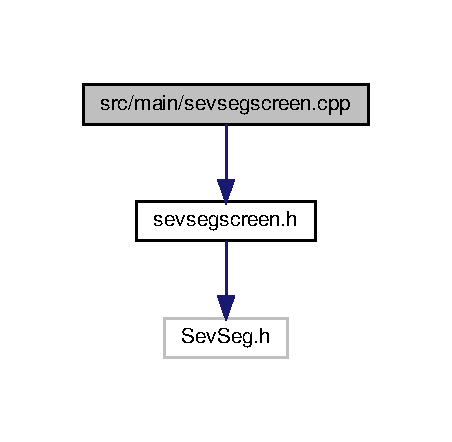
\includegraphics[width=217pt]{sevsegscreen_8cpp__incl}
\end{center}
\end{figure}


\subsection{Detailed Description}
Definition of \hyperlink{class_sevseg_screen}{Sevseg\+Screen} class. 

\begin{DoxyAuthor}{Author}
Valentin Mercy (\href{https://github.com/vmercy}{\tt https\+://github.\+com/vmercy}) 
\end{DoxyAuthor}
\begin{DoxyVersion}{Version}
0.\+1 
\end{DoxyVersion}
\begin{DoxyDate}{Date}
2020-\/11-\/26
\end{DoxyDate}
\begin{DoxyCopyright}{Copyright}
Copyright (c) 2020 
\end{DoxyCopyright}

\hypertarget{sevsegscreen_8h}{}\section{src/main/sevsegscreen.h File Reference}
\label{sevsegscreen_8h}\index{src/main/sevsegscreen.\+h@{src/main/sevsegscreen.\+h}}


Declaration of \hyperlink{class_sevseg_screen}{Sevseg\+Screen} class.  


{\ttfamily \#include $<$Sev\+Seg.\+h$>$}\newline
Include dependency graph for sevsegscreen.\+h\+:\nopagebreak
\begin{figure}[H]
\begin{center}
\leavevmode
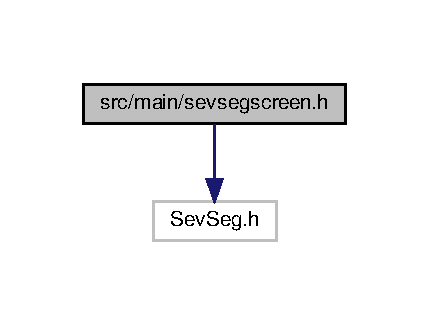
\includegraphics[width=206pt]{sevsegscreen_8h__incl}
\end{center}
\end{figure}
This graph shows which files directly or indirectly include this file\+:\nopagebreak
\begin{figure}[H]
\begin{center}
\leavevmode
\includegraphics[width=350pt]{sevsegscreen_8h__dep__incl}
\end{center}
\end{figure}
\subsection*{Classes}
\begin{DoxyCompactItemize}
\item 
class \hyperlink{class_sevseg_screen}{Sevseg\+Screen}
\begin{DoxyCompactList}\small\item\em \hyperlink{class_sevseg_screen}{Sevseg\+Screen} class is responsible for displaying content on a 7-\/segment display. \end{DoxyCompactList}\end{DoxyCompactItemize}
\subsection*{Macros}
\begin{DoxyCompactItemize}
\item 
\mbox{\Hypertarget{sevsegscreen_8h_a243b9da62168ae40123236a95376af07}\label{sevsegscreen_8h_a243b9da62168ae40123236a95376af07}} 
\#define {\bfseries S\+E\+V\+S\+E\+G\+\_\+\+T\+E\+S\+T\+\_\+\+D\+E\+L\+AY}~200
\end{DoxyCompactItemize}


\subsection{Detailed Description}
Declaration of \hyperlink{class_sevseg_screen}{Sevseg\+Screen} class. 

\begin{DoxyAuthor}{Author}
Valentin Mercy (\href{https://github.com/vmercy}{\tt https\+://github.\+com/vmercy}) 
\end{DoxyAuthor}
\begin{DoxyVersion}{Version}
0.\+1 
\end{DoxyVersion}
\begin{DoxyDate}{Date}
2020-\/11-\/26
\end{DoxyDate}
\begin{DoxyCopyright}{Copyright}
Copyright (c) 2020 
\end{DoxyCopyright}

\hypertarget{switch_8h}{}\section{src/main/switch.h File Reference}
\label{switch_8h}\index{src/main/switch.\+h@{src/main/switch.\+h}}


Declaration of switch class.  


{\ttfamily \#include \char`\"{}button.\+h\char`\"{}}\newline
Include dependency graph for switch.\+h\+:\nopagebreak
\begin{figure}[H]
\begin{center}
\leavevmode
\includegraphics[width=174pt]{switch_8h__incl}
\end{center}
\end{figure}
This graph shows which files directly or indirectly include this file\+:\nopagebreak
\begin{figure}[H]
\begin{center}
\leavevmode
\includegraphics[width=185pt]{switch_8h__dep__incl}
\end{center}
\end{figure}
\subsection*{Classes}
\begin{DoxyCompactItemize}
\item 
class \hyperlink{class_switch}{Switch}
\begin{DoxyCompactList}\small\item\em \hyperlink{class_switch}{Switch} class is responsible for managing a 2-\/positions switch input. \end{DoxyCompactList}\end{DoxyCompactItemize}


\subsection{Detailed Description}
Declaration of switch class. 

\begin{DoxyAuthor}{Author}
Valentin Mercy (\href{https://github.com/vmercy}{\tt https\+://github.\+com/vmercy}) 
\end{DoxyAuthor}
\begin{DoxyVersion}{Version}
0.\+1 
\end{DoxyVersion}
\begin{DoxyDate}{Date}
2020-\/11-\/26
\end{DoxyDate}
\begin{DoxyCopyright}{Copyright}
Copyright (c) 2020 
\end{DoxyCopyright}

\chapter{Example Documentation}
\hypertarget{_2home_2valentin_2_dropbox_2_a_v_i_o_n__r_c_2_prog_2_r_c_2src_2main_2control_8h-example}{}\section{/home/valentin/\+Dropbox/\+A\+V\+I\+O\+N\+\_\+\+R\+C/\+Prog/\+R\+C/src/main/control.\+h}
\hyperlink{class_control}{Control} class is responsible for translating \hyperlink{class_joystick}{Joystick}, encoder and button inputs into power, pitch, yaw and roll values \begin{DoxyNote}{Note}
Description of controls \+:
\begin{DoxyItemize}
\item C\+T\+R\+L1 \+: mode selector \+: Ground (off) / Flight (on))
\item C\+T\+R\+L2 \+: auto-\/thrust activation \+: Disable (off) / Enable (on)
\item C\+T\+R\+L3 \+: set auto-\/thrust to neutral (halfway)
\item C\+T\+R\+L4 \+: yaw activation \+: Disable (off) / Enable (on)
\item \hyperlink{class_encoder}{Encoder} \+:
\begin{DoxyItemize}
\item CW \+: auto-\/thrust cursor += get\+Setting(\+A\+U\+T\+O\+T\+H\+R\+U\+S\+T\+\_\+\+C\+U\+R\+S\+O\+R\+\_\+\+S\+T\+E\+P)
\item C\+CW \+: auto-\/thrust cursor -\/= get\+Setting(\+A\+U\+T\+O\+T\+H\+R\+U\+S\+T\+\_\+\+C\+U\+R\+S\+O\+R\+\_\+\+S\+T\+E\+P)
\item \hyperlink{class_switch}{Switch} (button) \+: reset auto-\/thrust to 0 (this is equivalent to temporarily disable auto-\/thrust) 
\end{DoxyItemize}
\end{DoxyItemize}

Description of control modes \+:
\begin{DoxyItemize}
\item Ground mode \+:
\begin{DoxyItemize}
\item Left joystick \+:
\begin{DoxyItemize}
\item X axis \+: nothing
\item Y axis \+: power (eventually reduced to map(power,0,255,0,get\+Setting(\+M\+A\+X\+\_\+\+G\+R\+O\+U\+N\+D\+\_\+\+P\+O\+W\+E\+R)) if get\+Setting(\+R\+E\+D\+U\+C\+E\+\_\+\+G\+R\+O\+U\+N\+D\+\_\+\+S\+P\+E\+E\+D) == true)
\end{DoxyItemize}
\item Right joystick \+:
\begin{DoxyItemize}
\item X axis \+: roll + yaw
\item Y axis \+: pitch
\end{DoxyItemize}
\end{DoxyItemize}
\item Flight mode \+:
\begin{DoxyItemize}
\item Left joystick \+:
\begin{DoxyItemize}
\item X axis \+: yaw
\item Y axis \+: power
\end{DoxyItemize}
\item Right joystick \+:
\begin{DoxyItemize}
\item X axis \+: roll
\item Y axis \+: pitch 
\end{DoxyItemize}
\end{DoxyItemize}
\end{DoxyItemize}

Description of auto-\/thrust \+:
\begin{DoxyItemize}
\item General case \+: power = cursor + map(joystick, min, max, halfway, max) //\+T\+O\+DO\+: check
\item Particular cases \+:
\begin{DoxyItemize}
\item When m\+\_\+auto\+Thrust\+Cursor = 0 \+: power = map(joystick, min, max, halfway, max)
\item When m\+\_\+auto\+Thrust\+Cursor = 128 (halfway) \+: power = joystick
\item When m\+\_\+auto\+Thrust\+Cursor = 255 (max) \+: power = max
\end{DoxyItemize}
\end{DoxyItemize}
\end{DoxyNote}

\begin{DoxyCodeInclude}

\textcolor{preprocessor}{#ifndef CONTROL\_H}
\textcolor{preprocessor}{#define CONTROL\_H}

\textcolor{preprocessor}{#include "\hyperlink{joystick_8h}{joystick.h}"}
\textcolor{preprocessor}{#include "\hyperlink{encoder_8h}{encoder.h}"}
\textcolor{preprocessor}{#include "\hyperlink{buzzer_8h}{buzzer.h}"}
\textcolor{preprocessor}{#include "\hyperlink{rgbled_8h}{rgbled.h}"}
\textcolor{preprocessor}{#include "\hyperlink{switch_8h}{switch.h}"}
\textcolor{preprocessor}{#include "\hyperlink{lcdscreen_8h}{lcdscreen.h}"}
\textcolor{preprocessor}{#include "\hyperlink{settings_8h}{settings.h}"}

\textcolor{preprocessor}{#define GROUND\_MODE 0}
\textcolor{preprocessor}{#define FLIGHT\_MODE 1}

\textcolor{preprocessor}{#define CONTROL\_IDLE 128}

\textcolor{keyword}{class }\hyperlink{class_control}{Control}
\{
\textcolor{keyword}{private}:
    \textcolor{keywordtype}{bool} m\_mode;
    uint8\_t m\_autoThrustCursor;

    \hyperlink{class_joystick}{Joystick} m\_leftJoy;
    \hyperlink{class_joystick}{Joystick} m\_rightJoy;
    \hyperlink{class_encoder}{Encoder} m\_encoder;
    \hyperlink{class_buzzer}{Buzzer} m\_buzzer;
    \hyperlink{class_r_g_b_led}{RGBLed} m\_rgbLed;
    \hyperlink{class_switch}{Switch} m\_CTRL1;
    \hyperlink{class_switch}{Switch} m\_CTRL2;
    \hyperlink{class_button}{Button} m\_CTRL3;
    \hyperlink{class_button}{Button} m\_CTRL4;
    \textcolor{comment}{//TODO: LCDScreen m\_screen;}
    \textcolor{keyword}{const} \hyperlink{class_settings}{Settings}* m\_p\_settings;
\textcolor{keyword}{public}:
    \hyperlink{class_control}{Control}();
    \textcolor{keywordtype}{void} \hyperlink{class_control_a435c342eba3a2598f3eb40e68fa1a263}{init}(\hyperlink{class_joystick}{Joystick} leftJoy\_p, \hyperlink{class_joystick}{Joystick} rioghtJoy\_p, 
      \hyperlink{class_encoder}{Encoder} encoder\_p, \hyperlink{class_switch}{Switch} gearSwitch\_p, \hyperlink{class_buzzer}{Buzzer} buzzer\_p, 
      \hyperlink{class_r_g_b_led}{RGBLed} rgbLed\_p, \textcolor{keyword}{const} \hyperlink{class_settings}{Settings}* p\_settings\_p);
    ~\hyperlink{class_control}{Control}();
    \textcolor{keywordtype}{void} \hyperlink{class_control_af7a1f77ddc2789d291e3193cfc046d50}{setMode}(\textcolor{keywordtype}{bool} newMode\_p);
    uint8\_t getPower();
    uint8\_t getPitch();
    uint8\_t getYaw();
    uint8\_t getRoll();
\};

\textcolor{preprocessor}{#endif}
\end{DoxyCodeInclude}
 
%--- End generated contents ---

% Index
\backmatter
\newpage
\phantomsection
\clearemptydoublepage
\addcontentsline{toc}{chapter}{Index}
\printindex

\end{document}
